%%%change to a4
\documentclass[a4paper,12pt]{article}\usepackage[]{graphicx}\usepackage[]{color}
%% maxwidth is the original width if it is less than linewidth
%% otherwise use linewidth (to make sure the graphics do not exceed the margin)
\makeatletter
\def\maxwidth{ %
  \ifdim\Gin@nat@width>\linewidth
    \linewidth
  \else
    \Gin@nat@width
  \fi
}
\makeatother

\definecolor{fgcolor}{rgb}{0.345, 0.345, 0.345}
\newcommand{\hlnum}[1]{\textcolor[rgb]{0.686,0.059,0.569}{#1}}%
\newcommand{\hlstr}[1]{\textcolor[rgb]{0.192,0.494,0.8}{#1}}%
\newcommand{\hlcom}[1]{\textcolor[rgb]{0.678,0.584,0.686}{\textit{#1}}}%
\newcommand{\hlopt}[1]{\textcolor[rgb]{0,0,0}{#1}}%
\newcommand{\hlstd}[1]{\textcolor[rgb]{0.345,0.345,0.345}{#1}}%
\newcommand{\hlkwa}[1]{\textcolor[rgb]{0.161,0.373,0.58}{\textbf{#1}}}%
\newcommand{\hlkwb}[1]{\textcolor[rgb]{0.69,0.353,0.396}{#1}}%
\newcommand{\hlkwc}[1]{\textcolor[rgb]{0.333,0.667,0.333}{#1}}%
\newcommand{\hlkwd}[1]{\textcolor[rgb]{0.737,0.353,0.396}{\textbf{#1}}}%
\let\hlipl\hlkwb

\usepackage{framed}
\makeatletter
\newenvironment{kframe}{%
 \def\at@end@of@kframe{}%
 \ifinner\ifhmode%
  \def\at@end@of@kframe{\end{minipage}}%
  \begin{minipage}{\columnwidth}%
 \fi\fi%
 \def\FrameCommand##1{\hskip\@totalleftmargin \hskip-\fboxsep
 \colorbox{shadecolor}{##1}\hskip-\fboxsep
     % There is no \\@totalrightmargin, so:
     \hskip-\linewidth \hskip-\@totalleftmargin \hskip\columnwidth}%
 \MakeFramed {\advance\hsize-\width
   \@totalleftmargin\z@ \linewidth\hsize
   \@setminipage}}%
 {\par\unskip\endMakeFramed%
 \at@end@of@kframe}
\makeatother

\definecolor{shadecolor}{rgb}{.97, .97, .97}
\definecolor{messagecolor}{rgb}{0, 0, 0}
\definecolor{warningcolor}{rgb}{1, 0, 1}
\definecolor{errorcolor}{rgb}{1, 0, 0}
\newenvironment{knitrout}{}{} % an empty environment to be redefined in TeX

\usepackage{alltt}



%%% Tex setup

%% General packages
\usepackage[margin=1in]{geometry} % set the margins
\usepackage{setspace} % load the [double|single]space commands
\usepackage{graphicx} % graphics

\usepackage{float}
\usepackage{multirow}
\usepackage{makecell}
\usepackage{rotfloat}

\newcommand{\specialcell}[2][c]{%
  \begin{tabular}[#1]{@{}c@{}}#2\end{tabular}}

%% BibTeX
\usepackage{natbib} % So we can use the APSR citation style
%\usepackage{hyperref} % Needed to process references with web
\usepackage{url} % links correctly
%\usepackage[authoryear,round,longnamesfirst]{natbib}
%% Math
\usepackage{amsmath,amsthm,amsfonts} % extended symbol set
\usepackage{bm} % Boldface support in math mode


%\renewcommand{\harvardurl}{URL: \url} %%make harvard and url work together

%%%%Figures



%% Generate the proposition, lemma, and hypothesis environments
\newtheorem{proposition}{Proposition}
\newtheorem{lemma}{Lemma}
\newtheorem{hypothesis}{Hypothesis}

%% Proper boldface for vectors
\makeatletter
\newcommand\vm[1]{% Vector or matrix
\bm{\mathrm{#1}}}

%% some useful math shortcuts
\newcommand{\Reals}{\mathbb{R}}
\newcommand{\argmax}{\operatornamewithlimits{argmax}}
\newcommand{\argmin}{\operatornamewithlimits{argmin}}
\newcommand{\var}{\text{var}}
\newcommand{\integ}[4]{\int_{#1}^{#2} \! #3 \, #4}

%% Various math shortcuts
\newcommand{\cN}{\mathcal{N}}
\newcommand{\cTN}{\mathcal{TN}}
\newcommand{\cIW}{\mathcal{W}^{-1}}
\newcommand{\cIG}{\mathcal{IG}^{-1}}
\newcommand{\cI}{\mathbb{I}}
\newcommand{\st}{{(t)}}
\newcommand{\stm}{{(t-1)}}
\newcommand{\suml}{\sum\limits}

%% Custom math shortcuts for this paper
\newcommand{\yctr}{{y_{ctr}}}
\newcommand{\ytctr}{{\tilde{y}_{ctr}}}
\newcommand{\br}{{\beta_r}}
\newcommand{\gryctrm}{{\gamma_{r,y_{ctr}-1}}}
\newcommand{\gryctr}{{\gamma_{r,y_{ctr}}}}
\newcommand{\grk}{{\gamma_{r,k}}}
\newcommand{\grkm}{{\gamma_{r,k-1}}}
\newcommand{\gr}[1]{{\gamma_{r,#1}}}
\newcommand{\zct}{{z_{ct}}}
\newcommand{\mctr}{{\mu_{ctr}}}

\newcommand\FramedBox[3]{%
 \setlength\fboxsep{1em}
 \fbox{\parbox[t][#1][c]{#2}{\small #3}}}




%%% Long title, but descriptive
\title{\Large{\textbf{Why Populism? How Parties Shape the Electoral Fortune of Populists}}}

\author{\normalsize{Darin Self and Allen Hicken}\thanks{Darin Self is a PhD Candidate at Cornell University. Allen Hicken is a Professor of Political Science at the University of Michigan -- Ann Arbor. This research project was supported by Riksbankens Jubileumsfond, Grant M13-0559:1, PI: Staffan I. Lindberg, V-Dem Institute, University of Gothenburg, Sweden; by Knut and Alice Wallenberg Foundation to Wallenberg Academy Fellow Staffan I. Lindberg, Grant 2013.0166, V-Dem Institute, University of Gothenburg, Sweden; as well as by internal grants from the Vice-Chancellor's office, the Dean of the College of Social Sciences, and the Department of Political Science at University of Gothenburg. We performed simulations and other computational tasks using resources provided by the Notre Dame Center for Research Computing (CRC) through the High Performance Computing section and the Swedish National Infrastructure for Computing (SNIC) at the National Supercomputer Centre in Sweden, SNIC 2017/1-407 and 2017/1-68. We specifically acknowledge the assistance of In-Saeng Suh at CRC and Johan Raber at SNIC in facilitating our use of their respective systems.}}


\date{}
\IfFileExists{upquote.sty}{\usepackage{upquote}}{}
\begin{document}
\singlespacing


\noindent \noindent \textbf{Varieties of Democracy (V--Dem)} is a new approach to conceptualization and measurement of democracy. The headquarters---the V-Dem Institute---is based at the University of Gothenburg with 17 staff. The project includes a worldwide team with six Principal Investigators, 14 Project Managers, 30 Regional Managers, 170 Country Coordinators, Research Assistants, and 3,000 Country Experts. The V--Dem project is one of the largest ever social science research-oriented data collection programs.


\vspace{175pt}

\noindent \noindent Please address comments and/or queries for information to:

\medskip
\noindent V--Dem Institute

\medskip
\noindent Department of Political Science 

\medskip
\noindent University of Gothenburg
\medskip

\noindent Spr\"{a}ngkullsgatan 19, PO Box 711
\medskip

\noindent SE 40530 Gothenburg
\medskip

\noindent Sweden
\medskip

\noindent E-mail: contact@v-dem.net



\vspace{250pt}



\noindent V--Dem Working Papers are available in electronic format at www.v-dem.net. 

\medskip
\noindent Copyright \copyright~2018 by the authors. All rights reserved.
\thispagestyle{empty}

\newpage

\maketitle
\thispagestyle{empty}

\newpage
\thispagestyle{empty}
\section*{Abstract}
Much of the literature on populism restricts itself to specific regional contexts. Due to this approach, theories of populism have difficulty explaining cross-regional similarities or differences (such as the prevalence of exclusive populist parties in Europe but inclusive parties in Latin America). Using cross-regional data and exploratory case studies from multiple regions, we provide evidence that the prevalence of populism in a given party system is a function of both party institutionalization and electoral institutions. The combination of these factors we term institutional hostility. In laying out our theory we identify three ways in which populist parties enter party systems and contest elections: populist entry, populist targeting and adaptation, and populist capture.

%%%Vdem preferred spacing
\newpage

\setcounter{page}{1}
\onehalfspacing

\section*{Introduction}
%%%%%%%%%%%%%%%%%%%%%%%%%%%%%%%%%%%%%%%%%%%%%%%%
%%%%%%%%%%%%%%%%%%%%%%%%%%%%%%%%%%%%%%%%%%%%%%%%
Recent events, such as the referendum for the United Kingdom to leave the European Union, the near election of a FP\"{O} candidate in Austria for President, and the election of Donald Trump, have sparked a wide spread discussion of populism and its (perceived) growing strength around the world. Elected officials and pundits within this discussion often speak of the rise of populism as a recent phenomenon, but this view is inaccurate. The presence of populism in both Europe and Latin America is nothing new. For decades now, populist parties such as the FP\"{O} in Austria or the FN in France have made steady electoral gains, while in Latin America populist parties and figures such as MAS under Evo Morales in Bolivia or Hugo Ch\'{a}vez in Venezuela surged to power in the 2000s. While the recent incidents of populism in electoral democracies is notable, it is not unprecedented. 
\par	
The presence of populism in Latin America and Europe is reflected in a large literature on the subject. Most of the work to date, however, has focused within a given region, with little work which draws comparisons directly between populism in Latin America and Europe, though with some important exceptions \citep{mudde2011voices, mudde2013exclusionary, hawkins2015mapping}. %are there any exceptions we want to footnote here% 
%these are the only ones I'm aware of
 The study of populism in Europe primarily focuses on radical-right populist parties \citep{betz1994radical, mudde2007populist}. In this context, populists  have generally secured some electoral gains or survived multiple electoral rounds and boast relatively organized and coherent parties. Research on populism in Latin America, on the other hand, often focuses on individual populist leaders who are associated with parties that are far weaker and more ephemeral than their European counterparts \citep{conniff2012populism}. We draw on these cross regional differences within a comparative framework to explore the factors that shape both the fortunes and forms of populist party politics.
\par
We argue that the magnitude of populists' success and the way in which populism manifests is dependent on what we call \textit{institutional hostility}.  Institutional hostility is a concept that captures the space within the political system for new populist parties, and is a function of: a) the degree of party institutionalization and b) the electoral institutions. Where parties are more institutionalized, the effectiveness of populists appeals diminish because existing parties are able to use their organizational prowess to mobilize both masses and elites for electoral gains. Likewise, Where the electoral system is more restrictive, populist parties will find it difficult to enter the electoral arena and win seats. Together these factors shape the hostility of the party system to populist challengers.
\par 
The pattern of institutional hostility also shapes the way in which populism is likely to manifest in a political system. At the highest levels of hostility, populist parties will be rare. At low and moderate levels hostility populism tends to manifest in one of three forms. Where the electoral system is permissive and existing parties are weak, populist parties can enter as mainline competitors for a large share of the vote. Where the electoral system is permissive but existing parties are institutionalized, populist parties are generally relegated as niche players in the party system. Finally, where the electoral system is restrictive but parties themselves are weakly institutionalized then the rise of populists is likely to come from factional challenges within existing parties.
\par 
To evaluate this argument we first use descriptive statistics to demonstrate that an association between institutional hostility and populist party success exists in both Western Europe and Latin America. We then use case studies along with quantitative data to illustrate how levels of and shifts in institutional hostility shape the success and pattern of populist party competition. 
\par
Our paper proceeds as follows: First, we provide greater background on populism in these Western Europe and Latin America. Next, we review the contested concept of populism and argue for an ideational, rather than material, conceptualization. After conceptualizing populism, we introduce our theory of how the the degree of institutional hostility shapes populism within a party system. Following our theory, we outline our research strategy and present quantitative and qualitative data to support our hypotheses. The purpose of this paper is to establish the plausibility of this argument and suggest areas for further research. After presenting our data we summarize our findings and conclude.
%%%%%%%%%%%%%%%%%%%%%%%%%%%%%%%%%%%%%%%%%%%%%%%%
%%%%%%%%%%%%%%%%%%%%%%%%%%%%%%%%%%%%%%%%%%%%%%%%
\section*{Background}
%%%%%%%%%%%%%%%%%%%%%%%%%%%%%%%%%%%%%%%%%%%%%%%%
%%%%%%%%%%%%%%%%%%%%%%%%%%%%%%%%%%%%%%%%%%%%%%%%
Populist parties and the purported rise of populism has attracted the attention of a growing number of scholars in recent years. In the  European context scholars have focused on describing the characteristics and levels professionalization of populist parties, explaining their level of success and durability, and analyzing the strategic interaction between populist and existing parties. \citep{betz1994radical, mudde2007populist, bale2010if, art2011inside}. For years, European populist parties had limited electoral success - usually functioning as exclusionary peripheral parties garnering small shares of electoral support. However, in recent years populist parties such as Syriza (Greece),  Podemos (Spain), and FP\"{O} (Austria), became major parties, won control of the government, and/or nearly captured the presidency. While these examples remain exceptional cases, populist parties throughout Europe have gained ground over the past decade and appear to be expanding \citep{mudde2017populism}.
\par
In general, populists and populist parties in the Americas have been more successful at the ballot box than their European counterparts, frequently winning presidential elections and capturing legislative majorities. There is a rich literature describing characteristics of these populists and exploring the reasons behind their rise to power. These include responses to neoliberal reforms \citep{weyland1999neoliberal,roberts1995neoliberalism,roberts2013market}, ethnic, indigenous, or class grievances \citep{webber2011rebellion,madrid2008rise}, and the rise of charismatic political leaders \citep{hawkins2003populism}. 
\par
Figure \ref{distribution} graphs the distribution of the presence of populism in party systems in both regions. The figure makes use of recent work by \citet{hawkins2015mapping} which weights electoral results for parties in Latin America and Western Europe by the strength of their populist rhetoric. A country's weighted populist score can run from 0\footnote{Party systems may receive a score of 0 for two possible reasons. First, parties that won any share of votes were scored as using no populist rhetoric. Second, if any set of parties within the system employ populist rhetoric but those parties receive no share of the vote the system's score is 0.} to 100.\footnote{All parties in the system use strong populist rhetoric.}  Figure \ref{distribution} illustrates that populism is more common in Latin American party systems than Western Europe. 
\par
%%%%%%%%%%%%%%%%%%%%%%%%%%%%%%
\begin{figure}[!htbp]%
\centering
\parbox{4in}{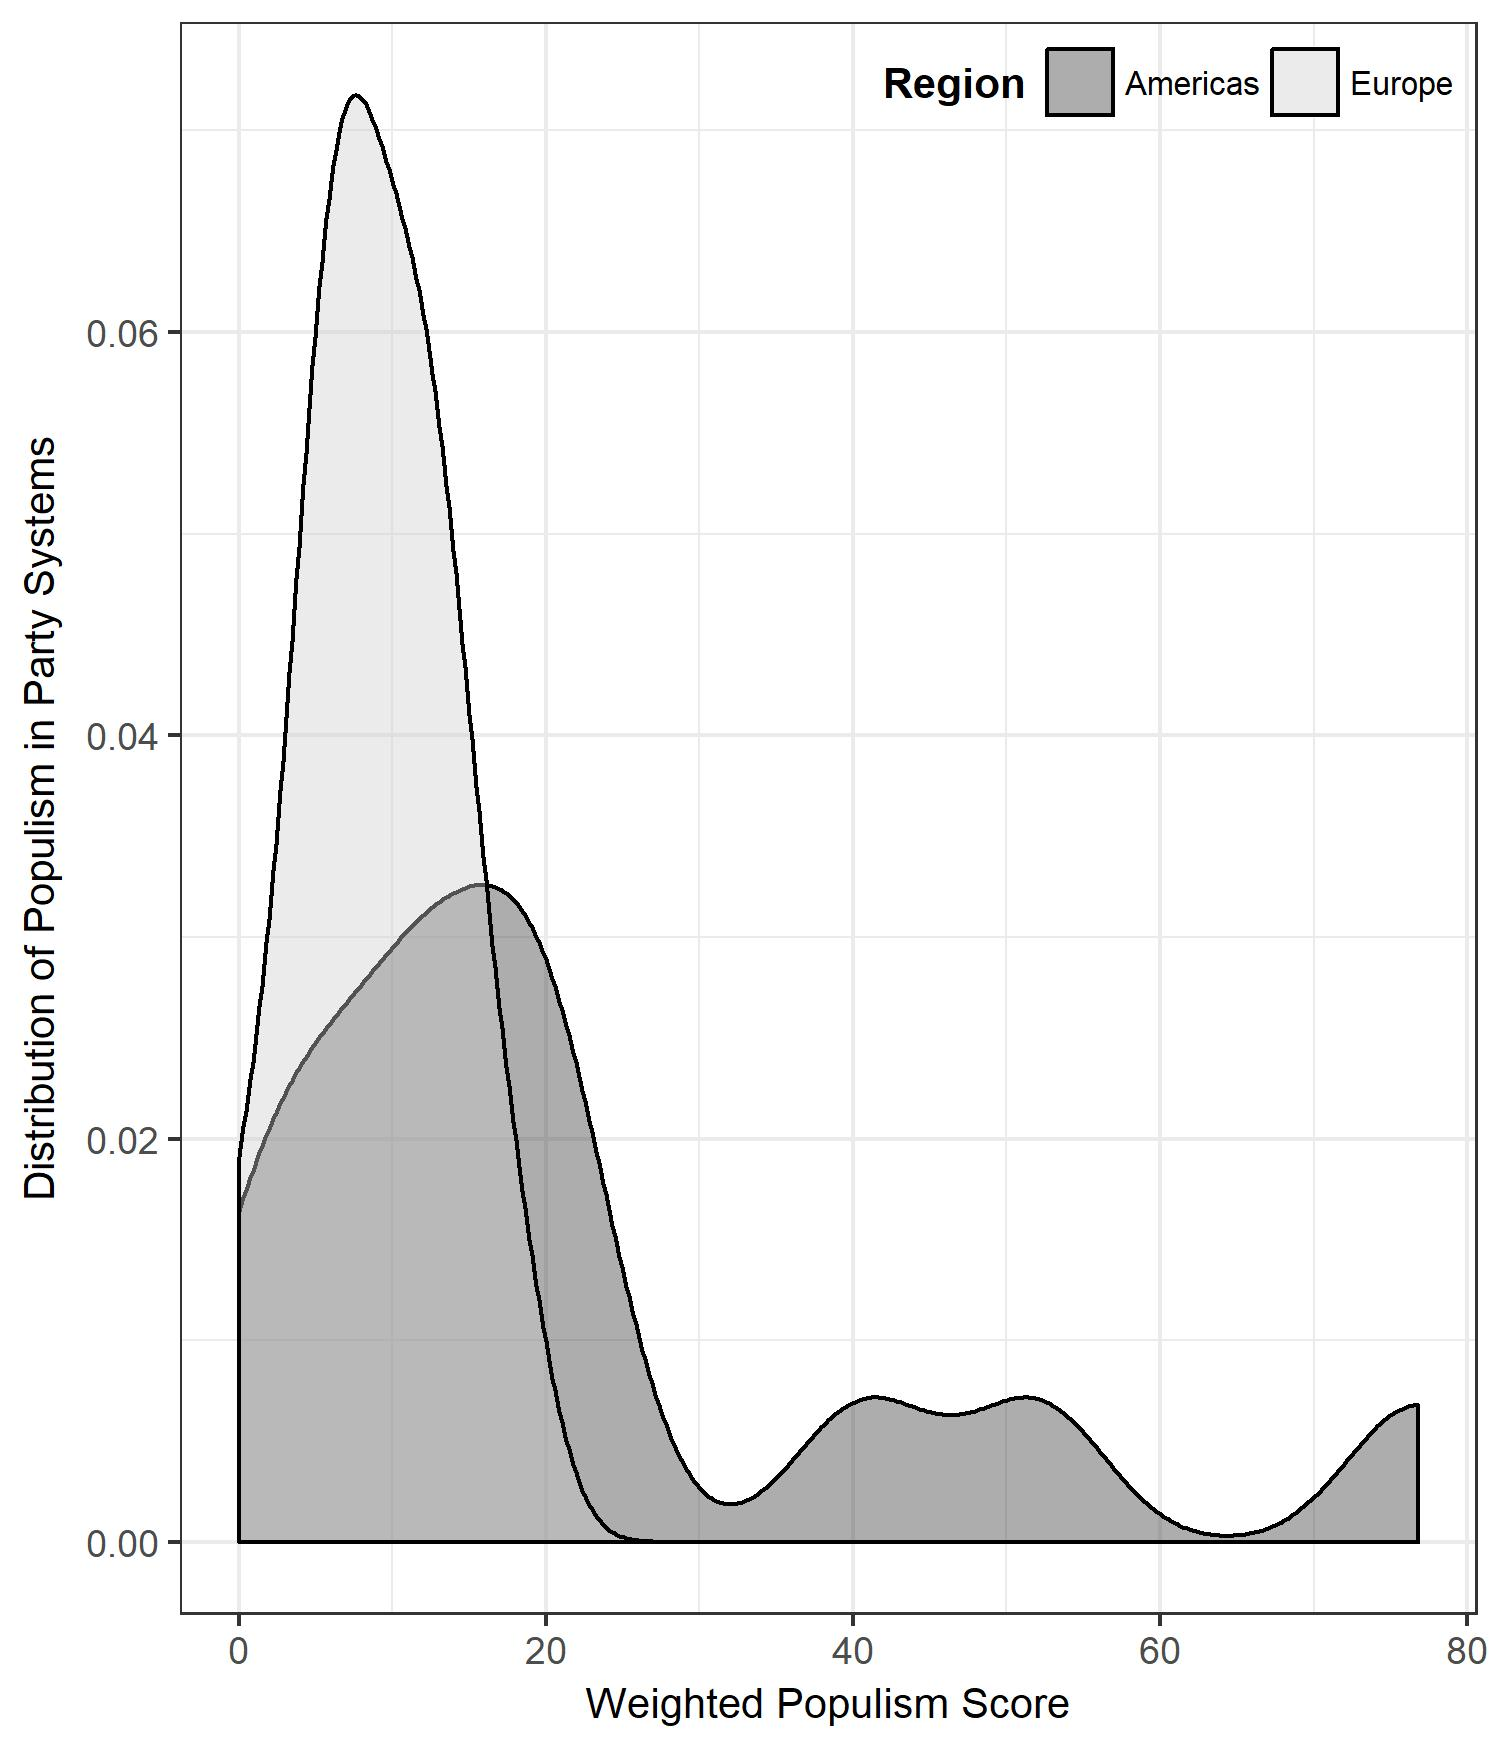
\includegraphics[width=100mm, height = 80mm]{fig1.jpg}}%
\qquad
\caption{Distribution of Populism in Latin American and Western European Party Systems}%
\label{distribution}%
\end{figure}
%%%%%%%%%%%%%%%%%%%%%%%%%%%%%%
Most European party systems have populism scores under 20, while 20 is nearly the modal score in Latin America. The variation of populism across Latin America is quite striking.  The strongest populist parties, by these criteria, are found in Venezuela, Bolivia, Ecuador, Argentina, and Peru. These results should come as no surprise and serve as a face validity check on Hawkins and Silva's method. While some the most populist party systems are found in Latin America, so too are some of the least populist party systems. The latter include Mexico, Paraguay, and Uruguay \citep{hawkins2015mapping}.
\par
What explains the variation of populism in party systems both within and between regions? With important exceptions, most of the existing work has focused on single country cases, or, if comparing more than one case, has remained within a single regional context. Analysis of the variance in the electoral performance of populist parties within and across regions has been comparatively under-studied. That is beginning to change with recent work by the likes of Cas Mudde, Crist{\'o}bal Kaltwasser, Kirk Hawkins,  Bruno Silva, and others \citep{mudde2011voices, mudde2013exclusionary, hawkins2015mapping}. These scholars have taken seriously the challenge of cross regional comparison and have begun to develop theories and tools to help make such comparison possible. This paper builds on these comparative approaches to present a genuinely comparative theory of populist party success.
\par
Specifically, we identify one factor that helps explain the variation in populist party success. We argue that the variation in the success of populist parties is partially a function of variation in institutional hostility. Institutional hostility refers to the extent to which there is opportunity or space in the party and electoral environments for new (populist) parties to emerge. As we discuss in more detail below, institutional hostility is a product of system level, inter-party, and intra-party factors. We expect that as individual political parties become more institutionalized and/or electoral institutions become more restrictive (high institutional hostility), the probability that populist parties will succeed diminishes, thereby reducing the expected payoff to adopting a populist strategy. By contrast, weak or underinstitutionalized parties and/or the presence of more permissive electoral institutions (low institutional hostility) opens the political space for populist parties and appeals. 

\par
We argue that, shaped by the level of institutional hostility, populism manifests itself in party systems in three ways: populist entry, populist targeting and adaptation, and populist capture. \textit{Populist entry} occurs when institutional hostility is low. Where the electoral system is permissive and party institutionalization is sufficiently low, new parties may enter and immediately compete with, or even outmatch, other parties in the system. \textit{Populist targeting and adaptation} occurs where permissive electoral systems combine with institutionalized parties. In such environments populist parties can enter but must adapt and evolve in order to compete with institutionalized parties. Lastly, \textit{Populist capture} occurs in environments where restrictive electoral rules combine with weak parties. Where populists arise in such systems it will be by taking control of an existing, factionalized party, rather than by entering as a new party. We discuss these three patterns of populist contestation in greater detail later.
%%%%%%%%%%%%%%%%%%%%%%%%%%%%%%%%%%
\section*{Populism: A Slippery Concept}
%%%%%%%%%%%%%%%%%%%%%%%%%%%%%%%%%%
Populism is one of the most contested concepts in the social sciences and is notoriously difficult to apply consistently \citep{roberts1995neoliberalism, roberts2003social, hawkins2015mapping, weyland2001clarifying}. Populism has frequently been associated with robust redistributive policies that are set against global liberalism and is often employed by academics, pundits, and politicians as a euphemism for leftist policies. However, the resurgence of populism in the 1980s and 1990s challenged the classical conceptualization of populism as populists did not limit themselves to leftist policies \citep{weyland2001clarifying, roberts2016newsletter}. Fittingly, debate on the formulation of populism as a concept in political science now centers on two opposing notions of what populism is. On one side of the argument authors propose a concept rooted in the form of elite-mass linkages and mobilization \citep{weyland2001clarifying, roberts2014populism}. By contrast,  the other approach focuses on the discursive rhetoric of populists \citep{mudde2007populist, hawkins2015mapping}.
\par
The elite-mass linkages approach to populism posits that populism is not simply tied to policy programs but instead to the nature of political organization. Under this framework, populists gain electoral support by creating large, cross-cutting, hierarchical, yet unorganized bases \citep{weyland2001clarifying}. \citet{roberts2015populism} argues that populism is a top-down, elite expropriation of mass mobilization that elites exploit for electoral and political gain. Roberts' conceptualization of populism is deeply rooted in the Latin American experience where populists step over the ashes of political parties whose downfall was brought about by the decoupling of parties from society. In these instances populists need only to push open an unlocked door into a party system where existing parties can no longer able mobilize the masses through a party apparatus. 
\par

In light of the Latin American experience this conceptualization of populism has merit. Because political parties in some Latin American states are relatively weak \citep{levitsky2016challenges} individuals can compete in the electoral arena without building a party. Why pay the costs of building a party when you can mobilize the masses for electoral gain without one? This conceptualization, however, encounters problems when applied to European cases where political parties remain crucial to electoral success and the elite subjugation of the masses is less pronounced. 
\par
Seeking to explain populism in Europe, \citet{mudde2007populist} writes from a tradition of populism that appears quite different than the Latin American experience. The European experience with populism has a number of key distinctions that require a different conceptualization of populism. First, and perhaps most importantly, European populists differ significantly from their Latin American counterparts in that they tend to develop robust party organizations. Another crucial distinction is the tendency of these parties to be right-wing parties with a strong exclusive nationalistic bent. Exclusive populist movements or parties seek to reinforce material, political, and symbolic dimensions within certain social groups while inclusive populist parties or movements seek to cross-cut material, political, and symbolic social groups \citep{mudde2013exclusionary}. 
\par
To conceptualize populism in Europe, \citet{mudde2007populist} and \citet{mudde2013exclusionary} frame populism as a discursive concept. In this framework, populism is a view of the world, expressed through discourse, with two opposing forces; the people - who embody the moral good - and the corrupt elite who conspire against the people. Building off of Mudde's ideational concept, \citet{hawkins2012measuring} define populism as a "\textit{Manichean approach to the political world that equates the side of Good with the putative “will of the people” and the side of Evil with a conspiring elite}" (2012, 2). 
\par
For \citet{ostiguy2009high, ostiguy2009highlow, ostiguy2013flaunting} populism is not necessarily a construct of how the world is viewed but a function of how the populist signals their closeness to the people. \citet{ostiguy2013flaunting} argues that populists relate to the people by flaunting the low - behaving or speaking in a way that sets them apart from the elite and allows them to be more closely related to the people. By way of example, consider two well-known Western politicians: David Cameron and Donald Trump. Cameron, an Oxford educated British politician speaks and behaves like a member of the cultural elite and adheres to conventional rules and procedures. Trump, by contrast, flaunts the low and appeals to "the people" by using coarser language and rhetoric filled with insults towards elites while dismissing norms and institutions. 
\par
Somewhat related to Ostiguy's approach to defining populism as a tool of signaling proximity to voters, \citet{moffitt2014rethinking, moffitt2016global} seek to resolve discrepancies between different conceptualizations of populism by framing it as a political style. In this way Moffit defines populism as "the repertoires of performance that are used to create political relations" \citep[p. 387]{moffitt2014rethinking}. 
\par
For the purposes of this study we adopt the second, discursive conceptualization of populism. We do this because it provides greater flexibility in comparing populists across regions of the world than is otherwise possible with an elite-mass approach. By adopting an elite-mass conceptualization of populism, we would limit ourselves to elite-dominated mass movements which are rarer in areas of the world where politics are well organized via political parties. We also do not favor one discursive conceptualization over the other. A \textit{prima facie} check of populists suggests that there is significant overlap between the Manichean \citep{hawkins2012measuring} and flaunting-the-low \citep{ostiguy2009high} types of populists. Often, in their attempt to construct a Manichean framing of the world, populists seek to relate to "the people" in an effort to set themselves apart from the traditional elites. 
%%%%%%%%%%%%%%%%%%%%%%%%%%%%%%%%%%
\section*{Populism's Party Problem}
%%%%%%%%%%%%%%%%%%%%%%%%%%%%%%%%%%
Many explanations for the rise of populism have been put forward -- with several centered on economic-focused explanations such as the growth of or backlash against globalization \citep{mughan2003economic, swank2003globalization, kriesi2006globalization, kriesi2008west} or neoliberalism \citep{roberts1995neoliberalism, weyland1999neoliberal}. While populist discourse often refers to economic grievances, we agree with others that populism is chiefly a political phenomena \citep{weyland2001clarifying, roberts2014populism}. Because populist is political phenomena within electoral democracies we argue that populism is closely linked with the nature of political parties. While we are among the first to explicitly link populism to party institutionalization, other scholars have certainly noted the role that parties play in the rise of populism,\footnote{Work on populism in Europe has also focused on how convergence to the center by mainstream parties opened the door to radical right populist parties \citep{kitschelt1997radical, abedi2002challenges, mudde2007populist, carter2011extreme}.} particularly in Latin America. Ken Roberts, for example, notes that bait-and-switch tactics used by party elites led to a programmatic delinkage between society and parties and contributed to the rise of populist politicians \citep{roberts1995neoliberalism, roberts2012politics, roberts2013market}. While we use a different conceptualization of populism than Roberts, we likewise view populism as highly influenced by the party system, specifically, the degree of party institutionalization. 
\par
Like other scholars we view party institutionalization as having two main components. First, institutionalized parties are characterized by value-infusion \citep{levitsky1998institutionalization}, meaning individual elites are willing to invest in the party to achieve their long term goals and as a result parties tend to be robust, cohesive organizations with professionalized staff and an establish label. Second, institutionalized parties have deep societal roots, with strong and stable links to identifiable groups of voters \citep*{mainwaring1995building}. Together, high levels of value infusion and strong societal roots produce institutionalized parties in which the short term particularistic interests of individual politicians are at times subordinate to the broader, longer term interests of the party \citep*{bizzarro2017v}.
\par
How does the degree of party institutionalization influence populism? Where institutionalization is high would-be populists face an electorate that is already tied to robust party organizations, leaving relatively few voters for populist entrants to mobilize. By contrast, where voter ties with political parties are weak and parties themselves ephemeral it is less costly for nascent populists to mobilize voters in support of their cause. We develop this argument in more detail below.
\par
In addition to the party system, we also recognize the role of the electoral system in shaping the incentives and capabilities of proto-populist. Permissive electoral systems provide a more welcoming environment for new entrants, including populist parties, compared to restrictive electoral systems, \textit{ceteris paribus}. We argue that party institutionalization combines with the nature of the electoral system to shape the incentives and capabilities of populists to mobilize voters and compete in the electoral arena. We label the combined effect of the electoral system and party institutionalization as the degree of \textit{institutional hostility}. \textit{Institutional hostility} shapes both the likelihood that populists will compete and be successful, and the form that populist competition will take. 
\par
Holding all else constant (economic environment, popularity of existing parties, popular disillusionment, etc.) the combination of these two factors shape the competitive environment and thus the opportunities for populists.\footnote{\cite{tavits2013post} explores how what she terms "environmental hostility" shapes the organization and party-building decision of new parties in post-communist democracies. Where environmental hostility is high (e.g. where public sentiment is hostile or where parties are at a disadvantage in terms of resources and reputation) parties have incentives to strengthen party organizations to compensate (p. 156).} To demonstrate how institutional hostility shapes the environment we outline three ways through which populists contest elections vis-\'{a}-vis existing parties in a polity: Populist Entry, Populist Targeting and Adaptation, and Populist Capture (See Table \ref{2x2}).
%%%%%%%%%%%%%%%%%%%%%%%%%%%%%%%%%%%%%%%%%%%%%%%%%%%%%%%%%%%%%%%%%%%%%%%%%%%%%%%%%%%%%%%%%%%%%%%%%%%
%%%%%%%%%%%%%%%%%%%%%%%%%%%%%%%%%%%%%%%%%%%%%%%%%%%%%%%%%%%%%%%%%%%%%%%%%%%%%%%%%%%%%%%%%%%%%%%%%%%
\begin{table}[h]
\centering
\scalebox{0.7}{
    \setlength{\extrarowheight}{2pt}
    \begin{tabular}{c >{\centering\arraybackslash}c|c|c|}

      & \multicolumn{1}{c}{} & \multicolumn{2}{c}{Degree of Institutionalization}\\
      & \multicolumn{1}{c}{} & \multicolumn{1}{c}{Low}  & \multicolumn{1}{c}{High} \\\cline{3-4}
      \multirow{2}*{\rotatebox{90}{Degree of Electoral System Restrictiveness~}}  & \specialcell[t]{\\ \\ Low} & \specialcell[t]{Low institutional hostility \\ (Populist Entry) \\ \\ \\ \\ Bolivia, Spain, and Venezuela} & \specialcell[t]{Moderate institutional hostility \\ (Populist Targeting \& Adaptation) \\ \\ \\ \\Austria and France} \\[18ex]\cline{3-4}
      & \specialcell[t]{\\ \\ High} & \specialcell[t]{Moderate institutional hostility \\ (Populist Capture)\\ \\ \\ \\ United States} & \specialcell[t]{High institutional hostility \\ (Populism is rare)} \\[18ex]\cline{3-4} 

    \end{tabular}
    }
    \caption{Types of Populism Manifested in Party Systems}
\label{2x2}
\end{table}
%%%%%%%%%%%%%%%%%%%%%%%%%%%%%%%%%%%%%%%%%%%%%%%%%%%%%%%%%%%%%%%%%%%%%%%%%%%%%%%%%%%%%%%%%%%%%%%%%%%
%%%%%%%%%%%%%%%%%%%%%%%%%%%%%%%%%%%%%%%%%%%%%%%%%%%%%%%%%%%%%%%%%%%%%%%%%%%%%%%%%%%%%%%%%%%%%%%%%%%

\subsection*{Low Institutional Hostility: Populist Entry}
When party institutionalization and barriers to entry are low the institutional environment for populist parties is ideal. Populists can easily enter the system and capitalize upon weak party-voter attachments and permissive electoral institutions. In short, we argue that when institutional hostility is low this provides the best opportunity for populist parties, and hence, we should expect populist parties to be more prevalent and more electorally successful, \textit{ceteris paribus}. 
\par
In cases where institutional hostility is low and political entrepreneurs enter the party system using a populist strategy we expect these parties to be more inclusive populist parties. Because voter linkages to pre-existing parties are weaker, entering populist parties may build a cross-cutting coalition, inclusive of many factions from the disaffected segments of society, more easily than in instances where pre-existing party-vote linkages are stronger. 
\par
\subsection*{Moderate Institutional Hostility Due to Low Party Institutionalization: Populist Capture }
What are our expectations where institutions are only moderately hostile--either a combination of weak parties with a restrictive electoral system, or strong parties with a permissive electoral system? We start with a system where parties are weakly institutionalized but the electoral system makes new party entry difficult. Because of the restrictive nature of the electoral system we expect the presence of populism in the party system to be less common--nascent populist parties typically cannot enter and capture large number of votes.   
\par
While rare, when populists emerge in this type of moderately hostile setting, the path to power is likely to be an intra-party one. Namely, populist leaders or factions wrest control of an existing party from other factions. Populist capture thus occurs when a populist (either a party outsider or leader of an internal party faction) attempts to gain control of the party, and non-populist party elites are unable to prevent the populist's rise. Where parties are highly institutionalized it is likely that party elites will be able to coordinate to prevent such capture. However, where party institutionalization is low, a lack of party cohesion makes it more likely that populist wings can successfully challenge party elites. 

\subsection*{Moderate Institutional Hostility Due to Permissive Electoral Institutions: Populist Targeting and Adaptation}
Where existing parties are institutionalized, the opportunities for what allows populist parties to enter and survive in systems are limited. First, existing parties already have high and durable levels of voter-party attachment, leaving relatively few unattached or weakly-attached voters available for populist mobilization. Second, institutionalized parties typically have a professional and robust organization that is effective at mobilizing their voters and beating back populist challenges. 
\par
However, where the electoral system is permissive, populist parties can find some success by targeting limited segments of society where party linkages are weaker. Populist targeting is typically accompanied by exclusive rhetoric and policy proposals aimed at voters at the margins of the existing political system. These kinds of appeals limit the appeal of these exclusive populists, placing a ceiling on their support, \textit{ceteris paribus}. If these new populists wish to compete against existing parties for more mainstream voters they must broaden their appeal and reduce the strength of their populist discourse. We call this strategy populist adaptation. 

 \subsection*{High Institutional Hostility: Few populist parties}
Should proto-populists seek to enter a system where institutional hostility is very high because of high levels of party institutionalization \textit{and} non-permissive institutions, they are unlikely to succeed. Winning a significant portion of the electorate will be difficult because it requires any new party to peel away a large number of voters that are strongly linked to existing parties. In addition, due to the highly restrictive nature of the electoral system they face the likely prospect of complete electoral failure with few to no seats. Given the hostile nature of the institutional environment populists should be least likely to emerge under these conditions.

%%%%%%%%%%%%%%%%%%%%%%%%%%%%%%%%%%%%%%%%%%%%
%%%%%%%%%%%%%%%%%%%%%%%%%%%%%%%%%%%%%%%%%%%%
\section*{Alternative Approaches}
%%%%%%%%%%%%%%%%%%%%%%%%%%%%%%%%%%%%%%%%%%%%
%%%%%%%%%%%%%%%%%%%%%%%%%%%%%%%%%%%%%%%%%%%%
Our argument points to parties and electoral restrictiveness as a cause of (the lack of) populism. We must also consider, however, that populism is actually a cause of party weakness or de-institutionalization. 
\par
If populism is a cause of party weakening or party de-institutionalization this would introduce a significant problem of endogeneity. In our model, we argue that parties are influential political institutions that are the best instruments for organizing and mobilizing voters. It is plausible that populism is actually a superior form of political mobilization, and that the rise of especially talented populists, such as Hugo Ch\'{a}vez, \textit{causes} the collapse of existing parties. Whether party weaknesses causes populism or populism undermines political parties is an empirical question that should be identified by looking at the timing of the rise of populists, which we do below. 
\par
Our argument also implies a puzzle that we must grapple with: \textit{if low institutional hostility allows populism to rise, why isn't populism ubiquitous in systems with low institutional hostility}? If populism is such a potentially powerful electoral tool, why then do we not observe more populism - especially where parties are weak? It is important to remember that populism is only one of many strategies politicians can use. Politicians may form parties, rely on personal wealth, use force, rely on clientelist networks or business ties, use nativist appeals, or use populism. None of these strategies are mutually exclusive and political entrepreneurs may use a mix of any set of strategies they believe to be the most advantageous. The payoff of populism, then, is dependent upon alternative forms of political organization and mobilization. Should alternative forms exist, political entrepreneurs may substitute to or away from populism depending on the instruments available to them. 
\par
Lastly, some may argue that the electoral strength of populists is dependent upon popular sentiment. Without popular disillusionment, the message of populists would ring-hollow. We agree that populist demand (i.e. popular disillusionment) may be a necessary condition and may help explain why populism isn't ubiquitous. Even where institutional hostility is low, if there is low demand for populism, populist parties will not find much electoral success. Our theory does not dismiss this argument and is actually complementary to it. Given a level of popular sentiment conducive to populist mobilization, we argue that the \textit{opportunities} for mobilization are a product of institutional hostility. Even where there is demand for populism, the extent to which populists can capitalize on populist sentiment is shaped by access to the system.
%%%%%%%%%%%%%%%%%%%%%%%%%%%%%%%%%%%%%%%%%%%%%%%%%%%%
%%%%%%%%%%%%%%%%%%%%%%%%%%%%%%%%%%%%%%%%%%%%%%%%%%%%
\section*{Research strategy}
%%%%%%%%%%%%%%%%%%%%%%%%%%%%%%%%%%%%%%%%%%%%%%%%%%%%
%%%%%%%%%%%%%%%%%%%%%%%%%%%%%%%%%%%%%%%%%%%%%%%%%%%%
The implication of our argument is that we should observe less electoral success by populists as institutional hostility increases. Our goal in this paper is not to precisely estimate a causal effect. Rather we seek to to establish the plausibility of our argument by presenting evidence of a link between institutional hostility and the presence of populism in any given party system. 
\par
To establish this link we follow a two-step research design. First, we make use of quantitative data. The purpose of this quantitative data is to move beyond mere description and demonstrate a cross-regional correlation between institutional hostility (particularly the level of party institutionalization) and populism. Because of the difficulty of identifying the exogenous relationship between party institutionalization and populism and data limitations, we choose not to use regression as any estimator will be biased.
\par
The second step in our research design is to use exploratory cases studies. The use of case studies serves two purposes. First, using cases studies provides a more nuanced view of the potential causal mechanisms through which variance in party institutionalization and electoral institutions may lead to changes in the degree of system-level populism. Second, case studies allow us to address the issue of endogeneity/reverse causality. %As previously mentioned, it is reasonable to believe that the rise of populism, or a particular populist, may lead to the de-institutionalization of individual parties or the party system as a whole.
By using exploratory case studies we pay particular attention to the timing of changes in the institutionalization of parties and the system as a whole vis-\`{a}-vis changes in the electoral fortunes of populists. 
%%%%%%%%%%%%%%%%%%%%%%%%%%%%%%%%%%%%%%%%%%%%%%
%%%%%%%%%%%%%%%%%%%%%%%%%%%%%%%%%%%%%%%%%%%%%%%
\section*{Data}
%%%%%%%%%%%%%%%%%%%%%%%%%%%%%%%%%%%%%%%%%%%%%%%
%%%%%%%%%%%%%%%%%%%%%%%%%%%%%%%%%%%%%%%%%%%%%%%
\noindent
\textit{Populism}\\
We measure populism using data from \citet{hawkins2015mapping} (Hereafter \textbf{HS}). \textbf{HS} treat populism as discursive and define it as discourse which treats politics as a dualistic struggle between the (morally good) people and the (morally evil or corrupt) elite. To measure populism, \textbf{HS} code party manifestos and selected speeches to produce a three point scale, ranging from zero to two. Zero indicates very little to no populism present, one indicates the presence of populist rhetoric but tempered by non-populist elements, and two indicates that a text is extremely populist. After coding is completed, scores are then aggregated through a multi-step process to create a single measure that indicates how prevalent populism is in a party system by weighting electoral results by each party's populism score.\footnote{See \citet{hawkins2015mapping} for a full explanation of how the data is generated.}  
\\
\noindent
\textit{Party Institutionalization} 
\par
To measure the average institutionalization of parties within the system, we use new data collected by the \textit{Varieties of Democracy Project} (Hereafter V-Dem), Our primary measure of average party institutionalization, is V-Dem’s index of Party Institutionalization (Hereafter \textit{PI}) \citep{bizzarro2018party}. \textit{PI} is an index created from five party-related components: party organization, branches, linkages, distinct party platforms, and legislative party cohesion.\footnote{For further discussion of the process please refer to \citet{bizzarro2017v} } \footnote{{PI} is normalized on a 0 to 1 scale, with higher values associated with higher levels of institutionalization. The V-Dem data includes observations for 193 countries with fairly regular coverage from 1900 to 2014.}
\par
As an alternative way to operationalize institutionalization we employ a measure of party strength developed by \citet{bizzarro2017v}. Party strength is an index that measures the extent to which political parties are characterized by: (1) permanent national party organizations, (2) permanent local party branches, (3) centralized mechanisms of candidate selection, (4) legislative cohesion, and (5) programmatic (rather than clientelistic) linkages to their social base. %\footnote{\citet{bizzarro2018party} also include party switching in their measure of party strength, however that indicator is no longer available in the latest version of V-Dem, so we have dropped it here.} 
The five indicators are aggregated through simple addition to form a Party Strength index, reflecting the expectation that each element of the index is partially substitutable. The index is also normalized on a 0 to 1 scale, with higher values associated with higher levels of party strength.
\par
We use these two measure of institutionalization to explore the correlation between the average institutionalization or strength of parties within the party system and the level of populism within the party system. Because the populism data is coded from elections near the year 2010, we average the past 10 years of \textit{PI} for each of the 25 countries available in \textbf{HS} . 
\\
\noindent
\textit{Electoral System Restrictiveness}
\par
To proxy for electoral system restrictiveness we use a new measure of district magnitude provided by \cite{selway2016system}. Selway and Self collected data on the district magnitude which accounts for electoral systems with multiple tiers in selecting seats for the legislature. Selway et al. measure the average district magnitude using the following formula below. 
\[
Avg District Mag = \frac{(Seats_1/Districts_1)}{Seats_1/ (Seats_1 + Seats_2)}+\frac{(Seats_2/Districts_2)}{Seats_2/(Seats_1 + Seats_2)}
\]
We use the log of \textit{AvgDistrictMag} as our measure of electoral system restrictiveness. We emphasize that this measure is a proxy for electoral system restrictiveness. One weakness of this proxy is that it does not account for the restrictiveness of the electoral system at the executive level. Some presidential or semi-presidential systems use rules that may make it easier for smaller parties to contest but this measure does not capture this. Instead, we capture the restrictiveness of the electoral system at the legislative level. 
\\
\noindent
\textit{Case Selection}
\par
In addition to quantitative data, we use exploratory case studies to probe the mechanisms through which institutional hostility affects the presence of populism as well as the direction and timing of this relationship. To explore the link between institutional hostility and populism we have selected six cases in two regions: the Americas and Western Europe. We have selected these regions to be consistent with our cross-national quantitative analysis and because countries within these regions provide variation in terms of the robustness of parties and party systems as well as the prevalence of populism. %\footnote{Further justification may be found in the Appendix.} 
\par
From the Americas we have selected Bolivia, the United States, and Venezuela. In Bolivia Evo Morales captured the MAS party, melded it with his significant grass-roots movements, and entered and came to dominate a relatively weak party system. The United States has a restrictive electoral system with moderately institutionalized parties. We focus on the 2016 U.S. election to demonstrate how populism can enter a seemingly stable party system through an under-institutionalized party. Finally, Venezuela is the quintessential story of populism in Latin America. Following significant political upheaval during the 1990s, Hugo Ch\'{a}vez entered a weakened party system with a new and weakly-institutionalized political party using his own brand of strong populism – Chavismo.
\par
In addition to the Americas we select three cases from Western Europe -- Austria, France, and Spain. We select from Western Europe because the region is commonly associated with relatively strong and institutionalized party systems. Austria and France each demonstrate how populist parties are largely disadvantaged in well-institutionalized party systems. In both cases populist parties entered as fringe parties and struggled to garner electoral support. Austria's FP\"{O} and France's FN parties have found greater electoral success as they have evolved and contested elections with a diluted populist brand. In Spain, despite massive economic upheaval, long established political parties have been able to maintain a significant hold on the electorate despite the rise of the new populist party, Podemos. 
%%%%%%%%%%%%%%%%%%%%%%%%%%%%%%%%%%%%%%%%%%%%
\section*{Cross-regional evidence}
We begin by exploring whether party institutionalization helps us understanding variation in populism. As previously mentioned, we have merged data from V-dem with cross-national data on populism from \textbf{HS}. %We present the summary statistics in Table 1 in the Appendix. 
\par
Table \ref{breakdown} summarizes the party and populism information for the two regions. On average, European democracies have stronger, more institutionalized parties compared to democracies in Latin America, and, as expected, this corresponds with less populism, whether measured by the average \textbf{HS} populism score, or the average vote share obtained by parties.
%%%%%%%%%%%%%%%%%%%%%%%%%%%%%%%%%%%%%%%%%%%%%%%%%%%%%%%%%%%%%%
\begin{table}[!htbp]
\centering 

  \caption{Breakdown of Populism and Party System Attributes by Region} 
  \label{breakdown} 

\begin{tabular}{@{\extracolsep{5pt}} ccc} 

\hline \\[-5ex] \\
Variable & Americas & Europe \\ 
\hline \\[-5ex] \\
PI & $0.70$ & $0.95$ \\ 
Party Strength & $0.62$ & $0.80$ \\ 
Populism & $22.32$ & $8.94$ \\ 
Vote Share & $26.71$ & $16.27$ \\ 
\hline \\[-1.8ex] 
\end{tabular} 

\end{table}
%%%%%%%%%%%%%%%%%%%%%%%%%%%%%%%%%%%%%%%%%%%%%%%%%%%%%%%%%%%%%%
We can get a better view of the relationship between party institutionalization and populism by plotting \textit{Populism} against our two measures of party institutionalization, \textit{PI} and \textit{Party Strength} (see Figure \ref{distribution}). Both panels in Figure \ref{fig2} shows a downward slope suggesting that as institutionalization increases, \textit{Populism} decreases.  
\par
It is also clear from Figure \ref{fig2} that populism varies more in the Americas compared to Europe, with Bolivia, Ecuador, and Venezuela each having high levels of populism while Mexico, the United States, and Uruguay each have low levels of populism. By contrast, each European party system is relatively institutionalized and has low levels of populism.\footnote{Because of data availability Greece and Spain were omitted from this sample. We suspect that the variance of \textit{Populism} would increase should these be included.} 

%%%%%%%%%%%%%%%%%%%%%%%%%%%%%%%%%%%%%%%%%%%%%%%%%%%%%%%%%%%%%%
\begin{figure}[!htbp]
\centering
\parbox{3in}{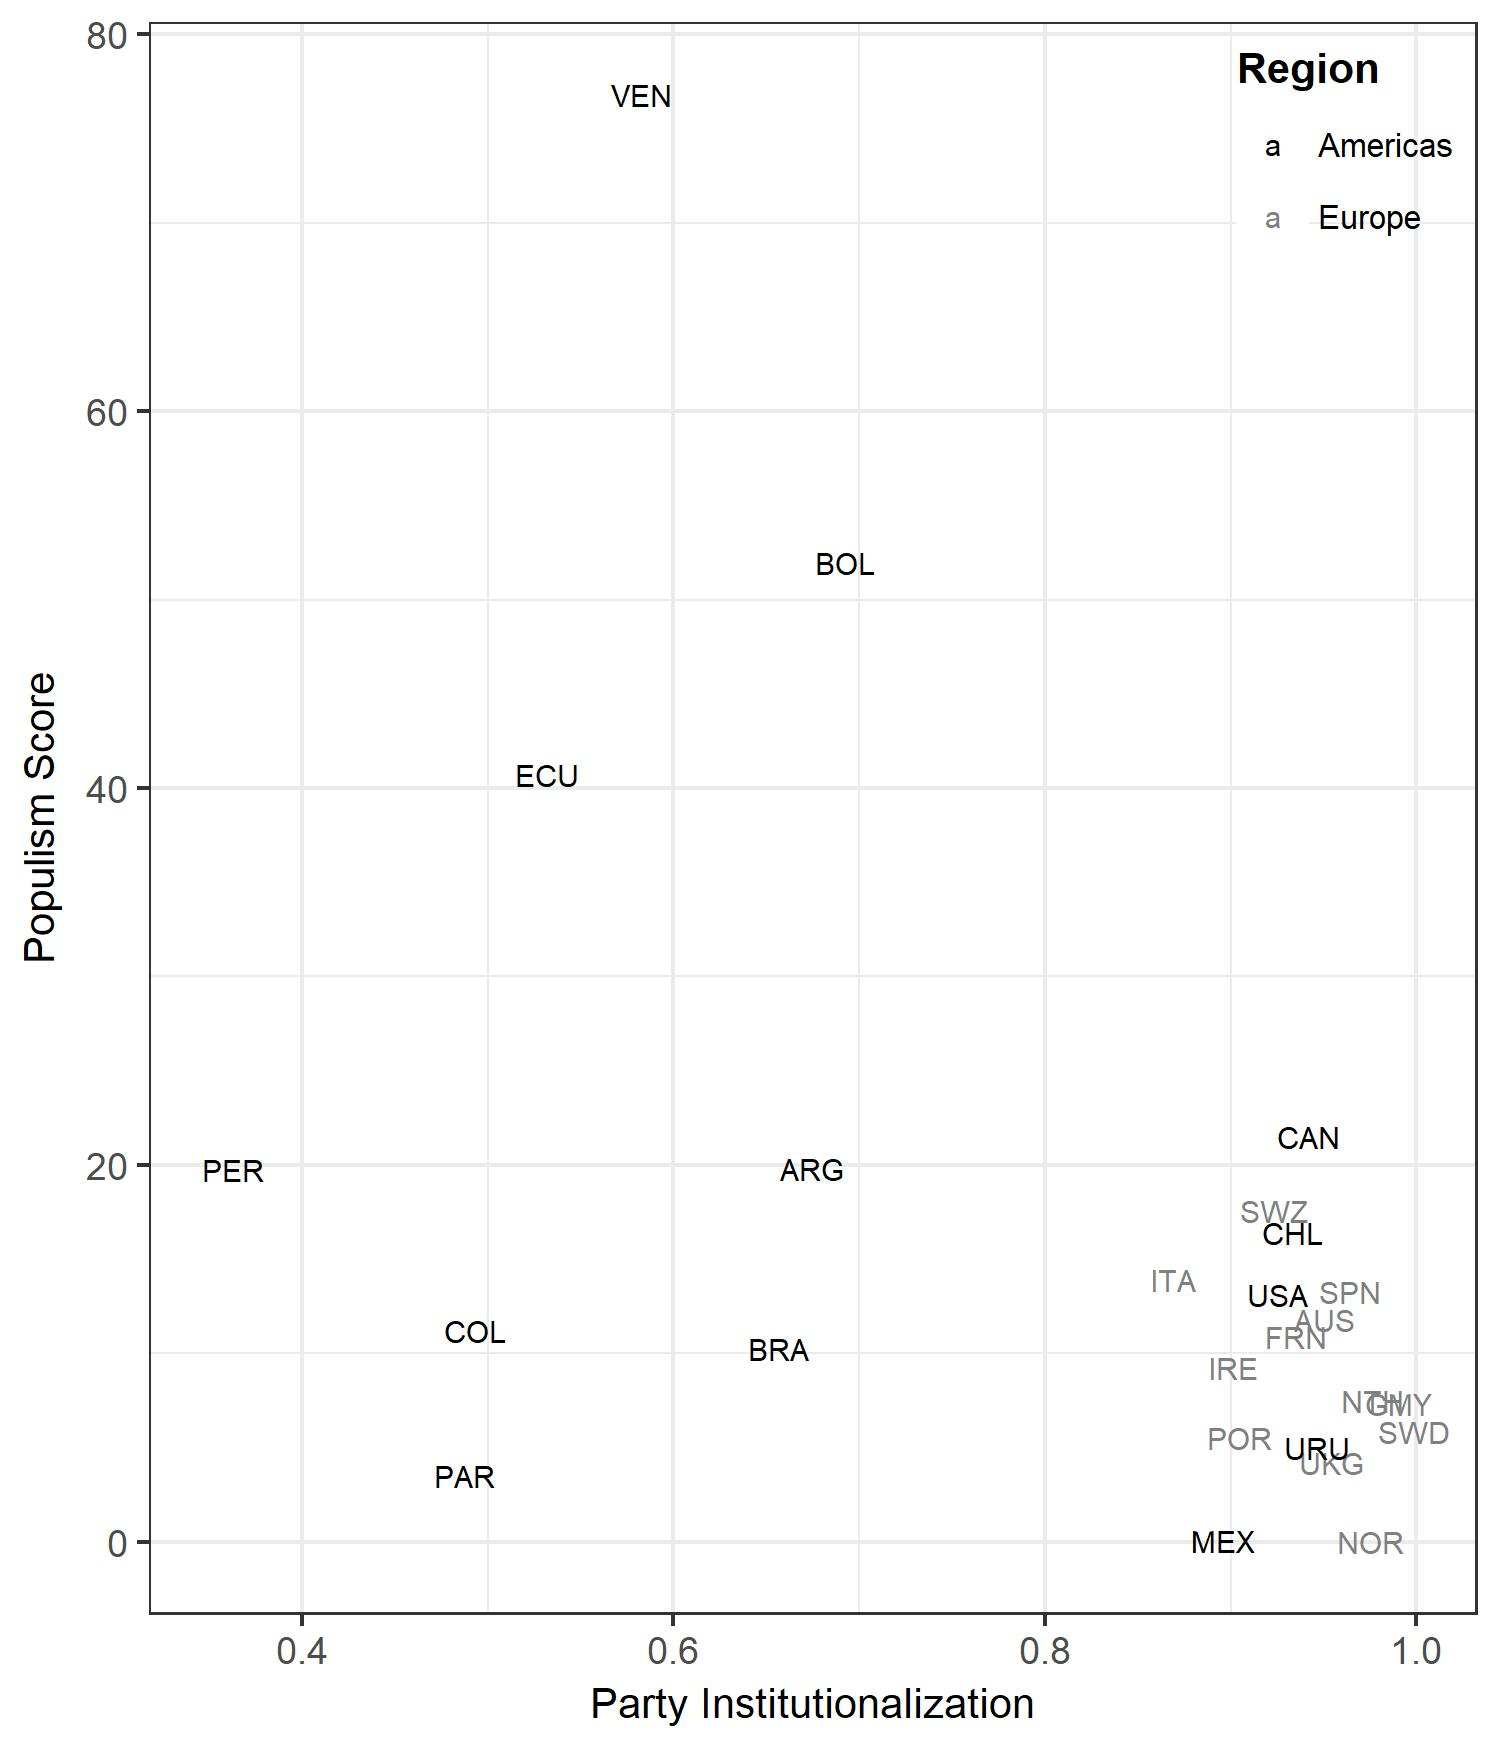
\includegraphics[width=80mm, height = 80mm]{fig2_1.jpg}}%
\qquad
\begin{minipage}{2.75in}%
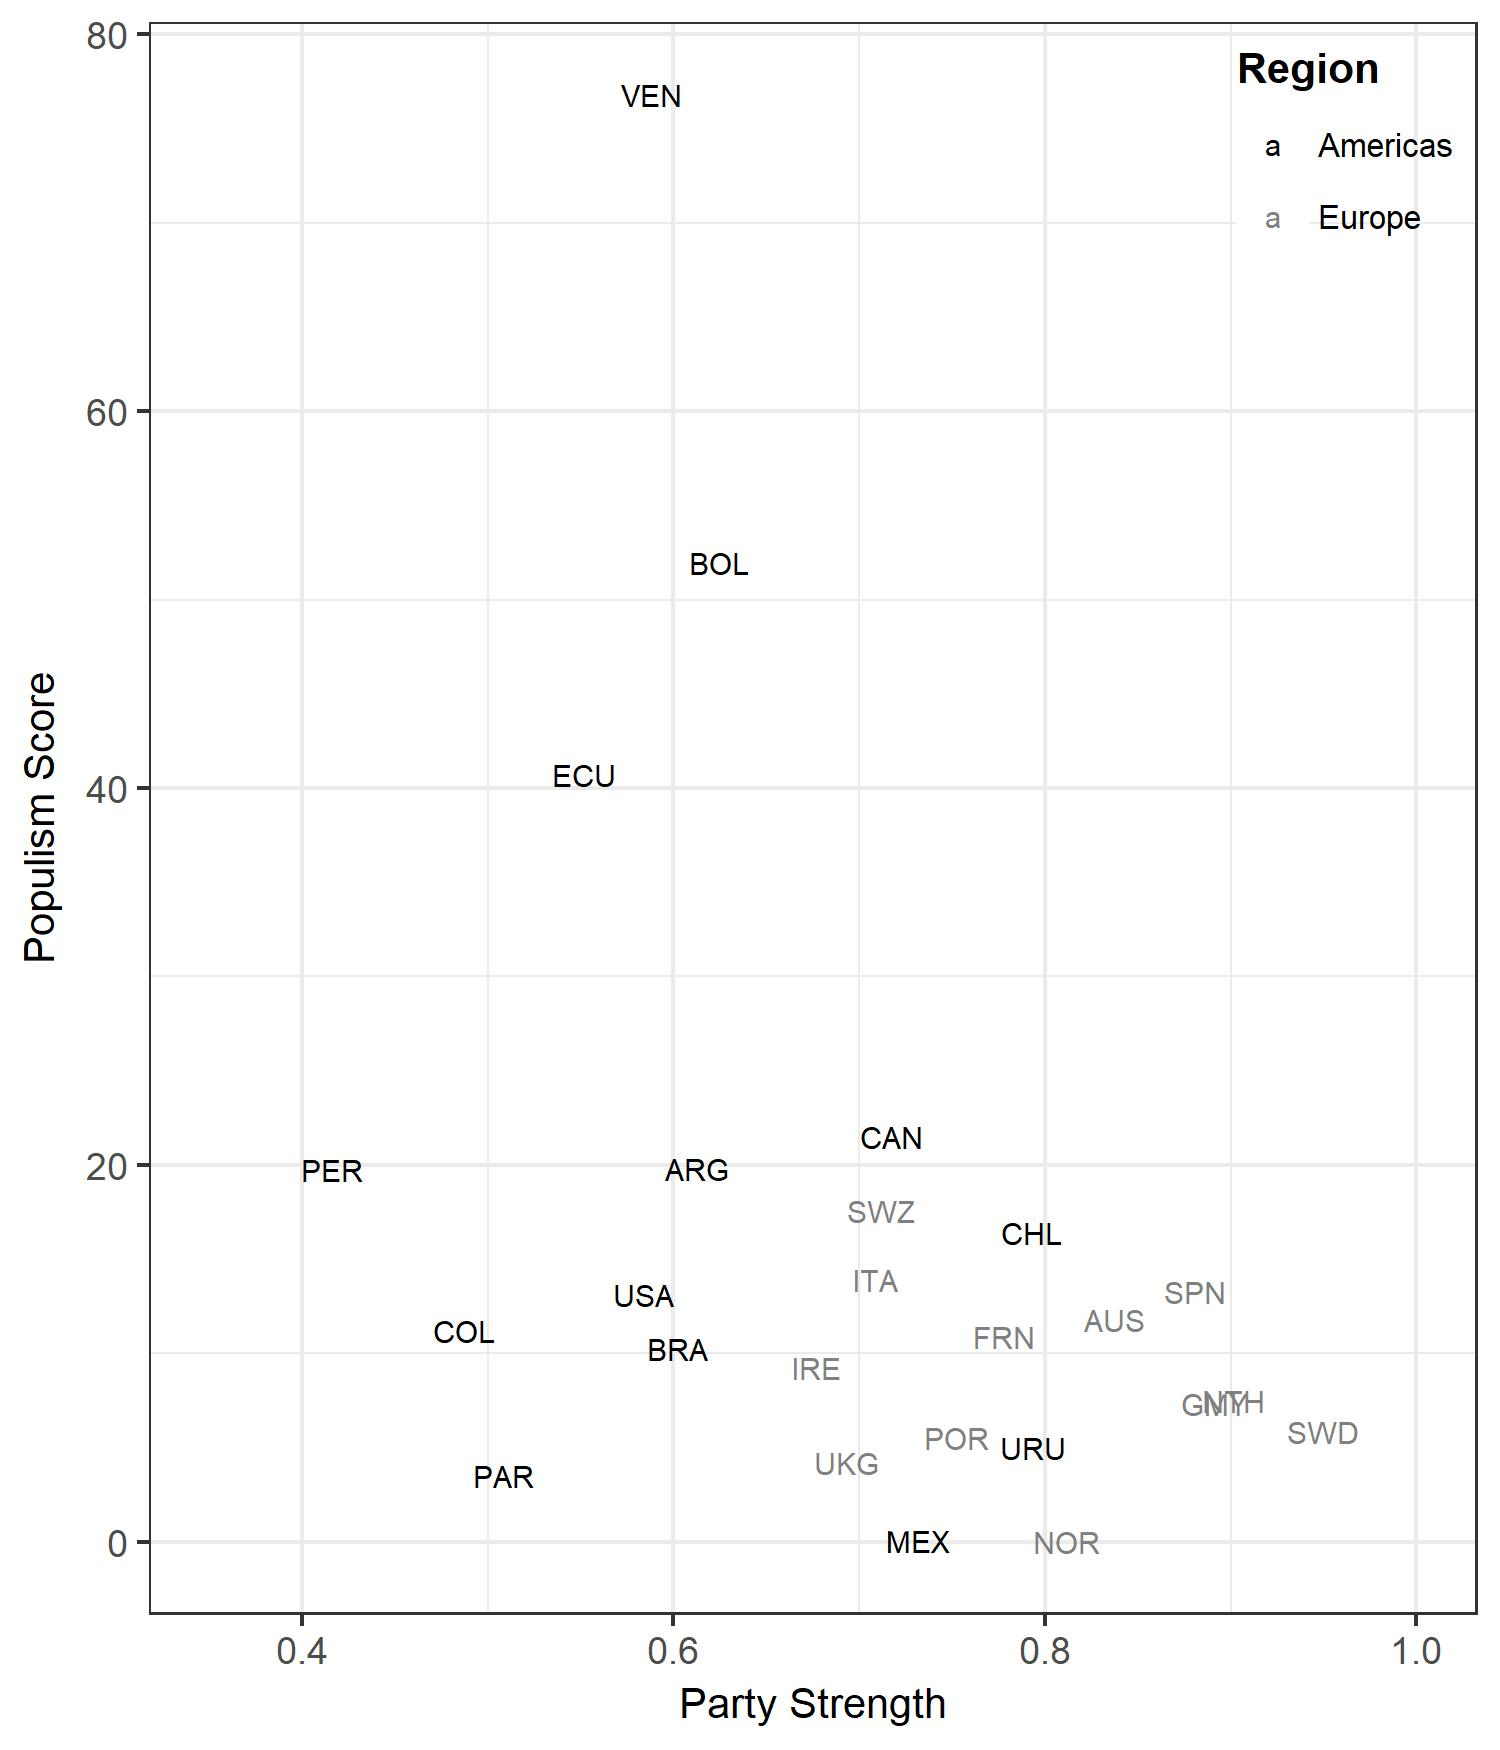
\includegraphics[width=80mm, height = 80mm]{fig2_2.jpg}
\end{minipage}%
\caption{Party Institutionalization or Strength and Weighted Populism Score}%
\label{fig2}%
\end{figure}
%%%%%%%%%%%%%%%%%%%%%%%%%%%%%%%%%%%%%%%%%%%%%%%%%%%%%%%%%%%%%%
\
\par
Next, we add the electoral system to the picture by combining \textit{Party Strength} and the log of \textit{AvgDistrictMag} to create an estimate of institutional hostility and plot the countries from our sample in Figure \ref{grid}. The horizontal line  separates countries with single and multi-seat constituencies. The vertical line represents the center of \textit{Party Strength} which has been normalized and centers on 0.73 - the median value of \textit{Party Strength} in the sample.\footnote{We use Party Strength here rather than PI because Party Strength incorporates information about how much control party leaders exercise over their ticket, which allows us to distinguish between parties systems with open primaries (e.g. the U.S.) and those without.} Based on our theory, we expect the figure to resemble the 2x2 depicted in Figure \ref{2x2}. The most populist cases should appear in the upper-left quadrant, where institutional hostility is low. Countries in the areas with moderate levels of institutional hostility should (upper right and lower left quadrants) should correspondingly lower levels of populism, with populists entering as exclusive outsiders in the upper left quadrant, and as intra-party populist insurgents in the lower left quadrant. Finally, populism should be relatively uncommon where institutional hostility is high (lower right).
%%%%%%%%%%%%%%%%%%%%%%%%%
\begin{figure}[!htbp]
\centering
\parbox{5in}{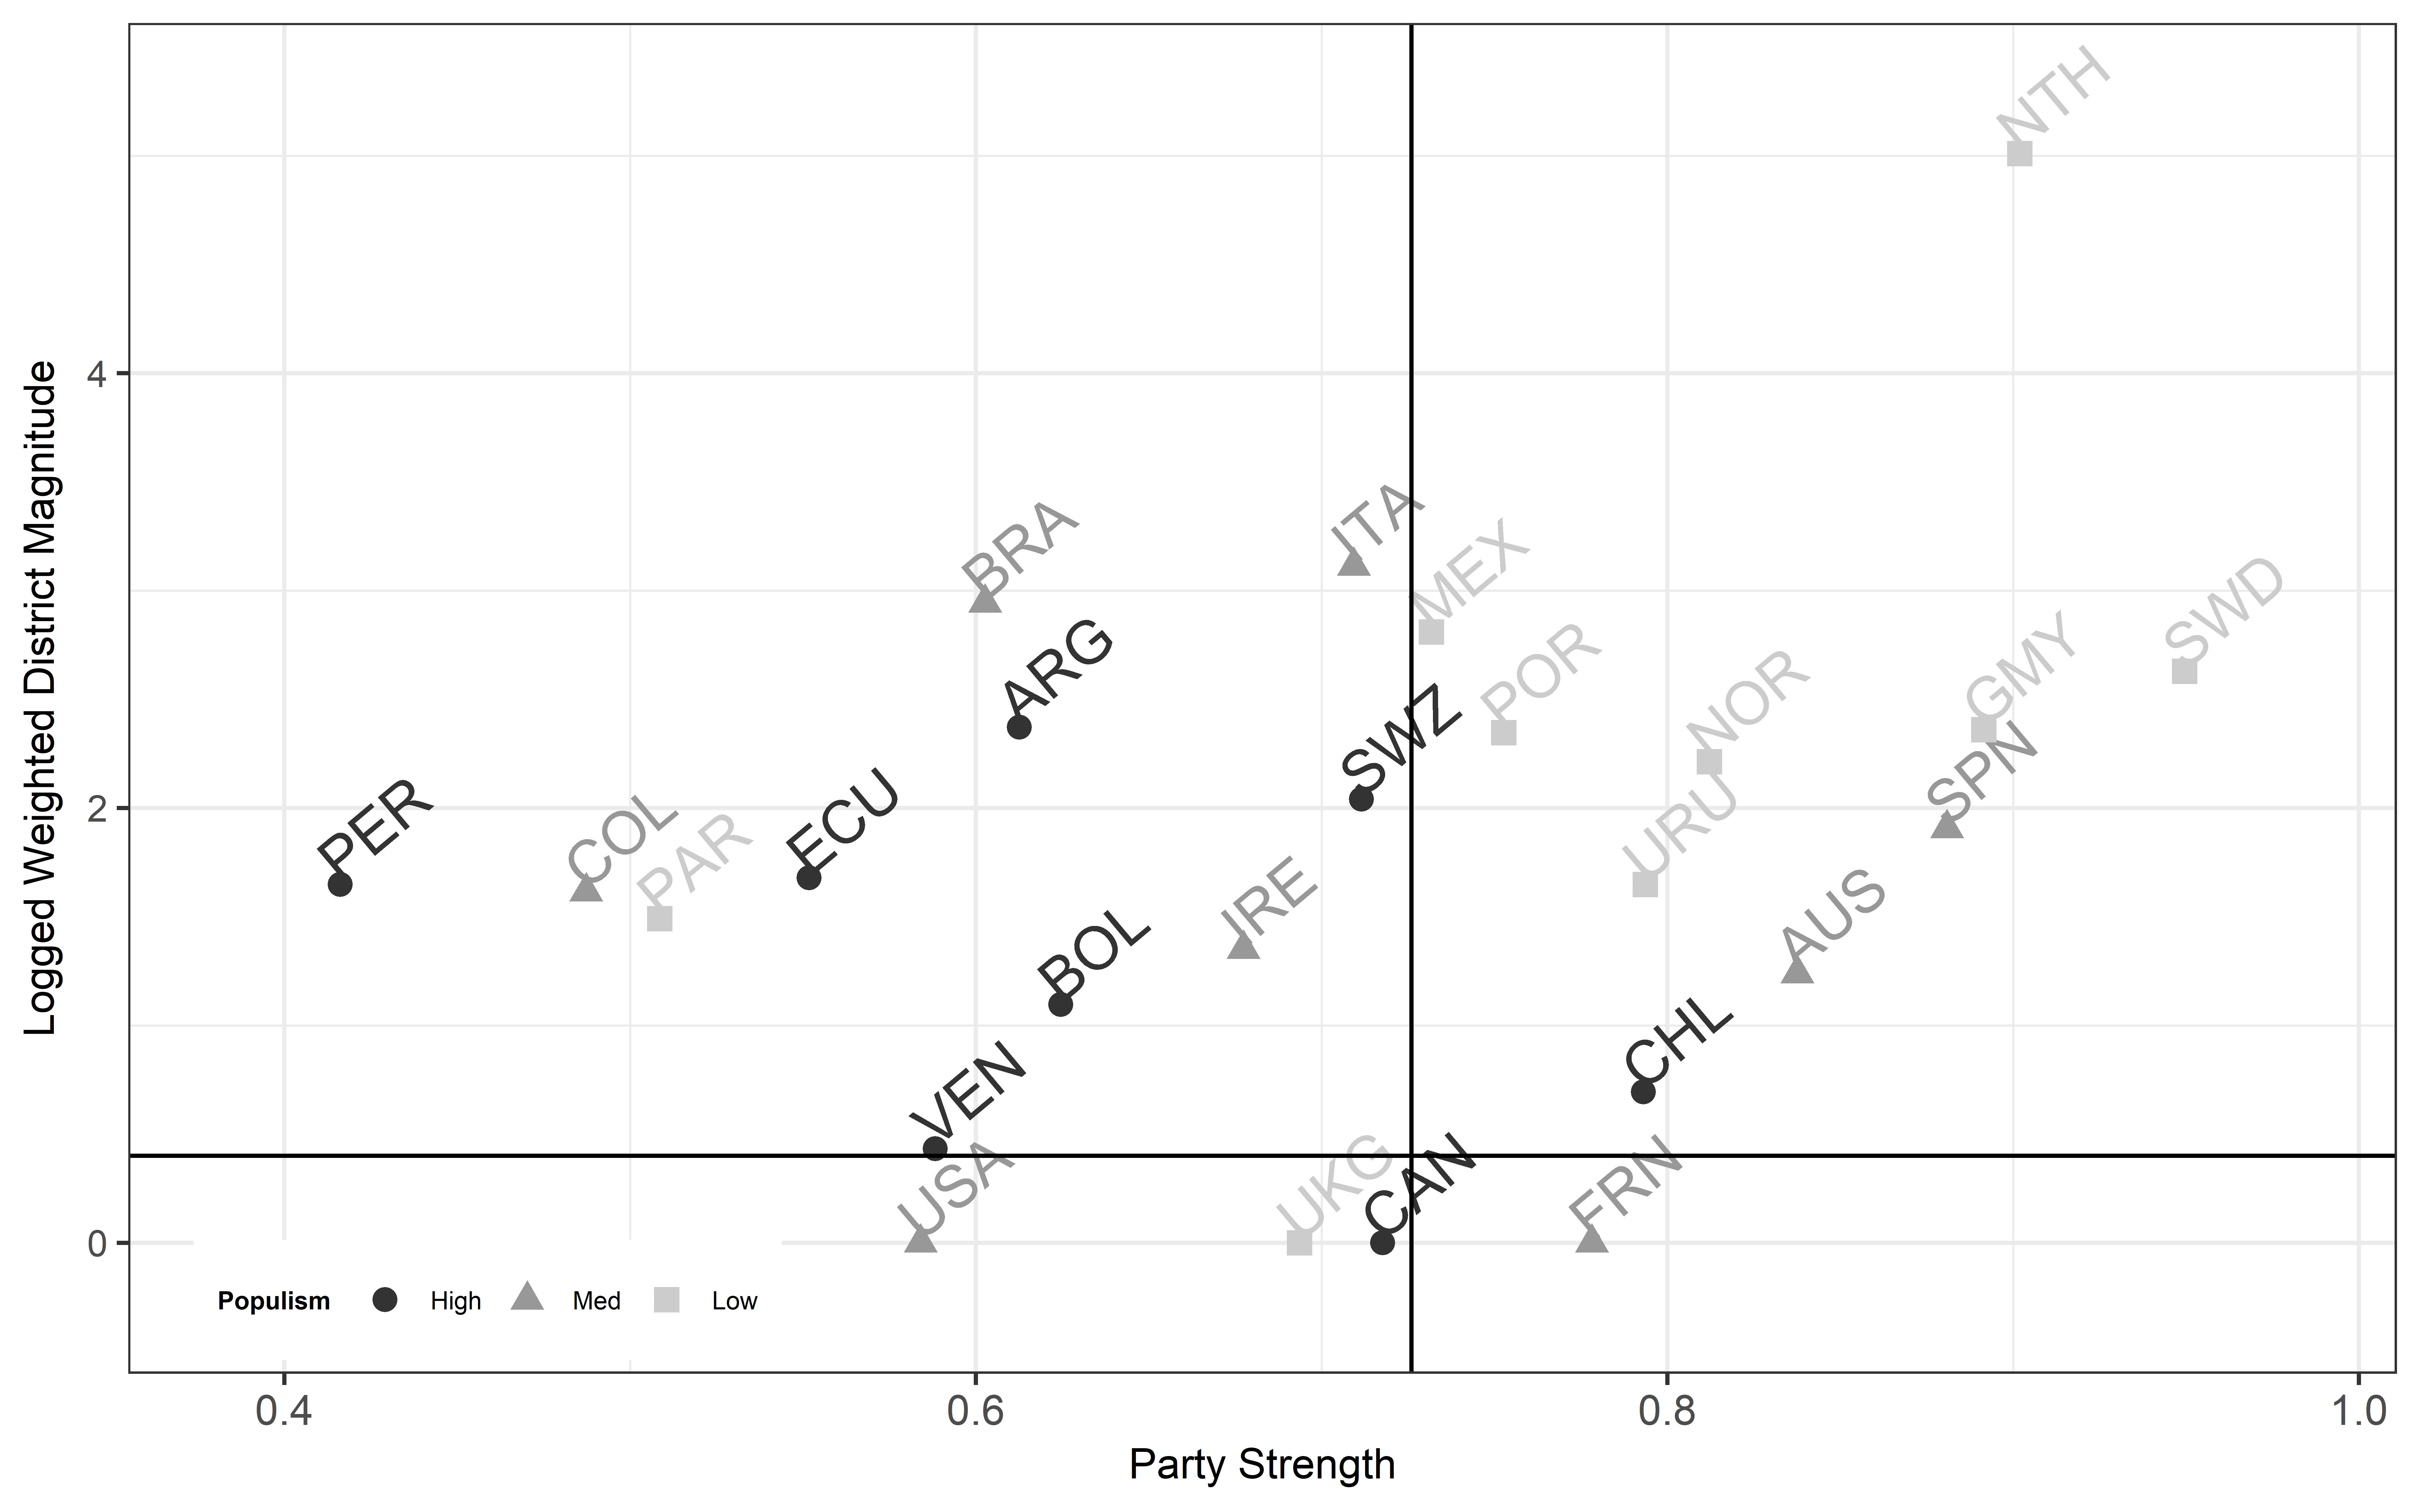
\includegraphics[width=120mm, height = 70mm]{fig3.jpg}}%
\qquad
\caption{Institutional Hostility and Populism in Party Systems}%
\label{grid}%
\end{figure}
%%%%%%%%%%%%%%%%%%%%%%%%
\par
The pattern of data in Figure \ref{grid} largely corresponds to our expectations. The countries with the highest populism scores are nearly all located in the top left quadrant. The average populism score for the upper left quadrant is 25.72--two to three times the score for the other quadrants. The upper right quadrant is home to mainly cases with medium to low levels of populism. Populism is comparatively rarer in our single member district cases, as expected, but it is more common where parties are weaker (i.e. the U.S. and Canada), and rare where institutional hostility is high (bottom right). The evidence also corresponds with our expectation regarding regional differences. Populism in Latin America is largely due to low institutional hostility, whereas populism in Europe occurs in an environment of strong parties and more permissive electoral systems. 
\par
The two most prominent outliers in Figure \ref{grid} are France and Canada.\footnote{Chile is another possible outlier. \citet{luna2011uprooted} argue that the Chilean party system is less institutionalized that it often appears in, which might account for its status.} This was anticipated. Both countries have electoral systems that are more permissive than implied by our simple measure of electoral system restrictiveness,  \textit{AvgDistrictMag}. While France uses single member districts, it also uses multiple rounds in both its legislative and executive elections, which makes the electoral system more permissive by fragmenting the party system \citep{birch2003two}. Thus, France would most likely be in the top-right dimension were we to use a different measure of electoral system restrictiveness. Turning to Canada, the high level or regionalism in the party system has regularly provided space for populist parties to enter and begin competing as regionally-based parties and later nationalize through party mergers \citep{behiels2010stephen}. During these mergers there is limited top-down control leading to a similar outcome, albeit a different process, of party capture found in the United States.
\par
%%%%%%%%%%%%%%%%%%%%%%%%%%%%%%%%%%%%%
\subsection*{Timing Populist Gains in Party Systems}
As previously mentioned, the possibility of reverse causality is theoretically plausible yet still an empirical question. Along with each of our brief case studies we use time-series plots of \textit{PI} and \textit{Party Strength} to investigate the timing of the rise of populist parties and address the issue of endogeneity. In each figure (Figures 4-6 and 7-10) we plot the time-series of \textit{PI} and \textit{Party strength} next to each other for comparison of within country time trends for each of the indicators. We plot the time-series for each indicator for each country for approximately 25 years.\footnote{In the European cases of Austria and France we extend the time horizon by 10 years to account for the first times that the FN in France and FP\"{O} in Austria became relatively competitive parties} along with the global average for democracies\footnote{To calculate the average we selected all country years where \textit{polity2} $\geq$ 6 and calculate the year average for \textit{PI} and \textit{Party Strength}} in order to compare the country-year trend with the global-year trend. We also highlight the years of the significant presence of populism in the party system with a gray background.
%%%%%%%%%%%%%%%%%%%%%%%%%%%%%%%%%%%%%%%%%%%%%%%%%%%%%%%%%%%%%%%%%%
%%%%%%%%%%%%%%%%%%%%%%%%%%%%%%%%%%%%%%%%%%%%%%%%%%%%%%%%%%%%%%%%%%
 \section*{Case Studies}
Because the quantitative data is not well suited for estimating causal effects we include several illustrative case studies to provide a preliminary exploration of the timing and type of populism present in these regions. We use these case studies to explore the causal mechanisms behind how institutional hostility influences the presence of populism in party systems. We also use these case studies to show how the strength of populism can fluctuate over time as a function of institutional hostility. 
\subsection*{Populist Entry}
%%%%%
\noindent
\textit{Venezuela} \\
We begin our cases studies with the prototypical populist case - Venezuela's Hugo Ch\'{a}vez. Prior to Ch\'{a}vez's ascendancy to the presidency in the late 1990s, the party system of Venezuela had experienced a decade-long collapse, despite previously being one of the most stable party systems in the region. If Venezuela had boasted one of the most institutionalized party systems, how did it come to collapse?
\par
Under pressure from the IMF and facing dire economic circumstances, Venezuela began to implement neo-liberal economic reforms in the late 1980s. These reforms were implemented by the AD (\textit{Acci\'{o}n Democratica}) party after winning the 1989 election; despite promises to avoid austerity \citep{dietz2007thaw}. This  "bait-and-switch" tactic served to programmatically dealign political parties \citep{roberts2013market}. The fractures in the party system began to show immediately in the next presidential election as Rafael Caldera split from his previous party \textit{COPEI} to run independently.\footnote{It is critical to note that all of this occurred well before Ch\'{a}vez contested an election.} Thus, within a few short years neo-liberal reforms had opened the first major cracks into the Venezuelan party system. 
\par
After a failed coup attempt and subsequent pardon, Hugo Ch\'{a}vez set to work organizing "Bolivarian Circles" in 1994. These circles were loosely tied, non-hierarchical, civic organizations that would later be critical to Ch\'{a}vez in mobilizing the electorate \citep{hawkins2003populism, roberts2006populism}. Despite the presence and use of these circles, however, Ch\'{a}vez never set out to develop these organizations into a well institutionalized party, instead leaving them to function as a quasi-party that would help mobilize voters. 
\par
If Ch\'{a}vez lacked an institutionalized party, how was he able to defeat parties which had had such a strong hold on the system? As discussed, the initial cracks to the party system arose after the bait-and-switch tactics of parties in the late 1980s and early 1990s. Not only did the introduction of IMF reforms force parties to renege on electoral promises, but neo-liberal reforms severely weakened corporatist linkages. In addition to these reforms, however, economic decline - especially the decline of oil revenue - also undermined parties' ability to make use of clientelistic linkages. This weakening of both corporatist and clientelistic linkages helped hasten the collapse of the existing party system \citep{roberts2003social, roberts2007latin}. 
\par
Due to the collapse of Venezuela's party system Ch\'{a}vez faced little institutionalized opposition. Thus, Ch\'{a}vez had little incentive to build his own institutionalized party and was able to combine extreme populist rhetoric with the loosely organized Fifth Republic Movement to easily defeat his weakened opposition \citep{hawkins2003populism}. The course of Venezuela's party collapse as the harbinger of the rise of Ch\'{a}vez is depicted in Figure \ref{venezuelapsi} below. In the late 1980s and early 1990s both \textit{PI} and \textit{Party Strength} begin to decline, providing an inviting environment for populist entry.  
\\
\begin{figure}[H]%
\centering

\parbox{2.5in}{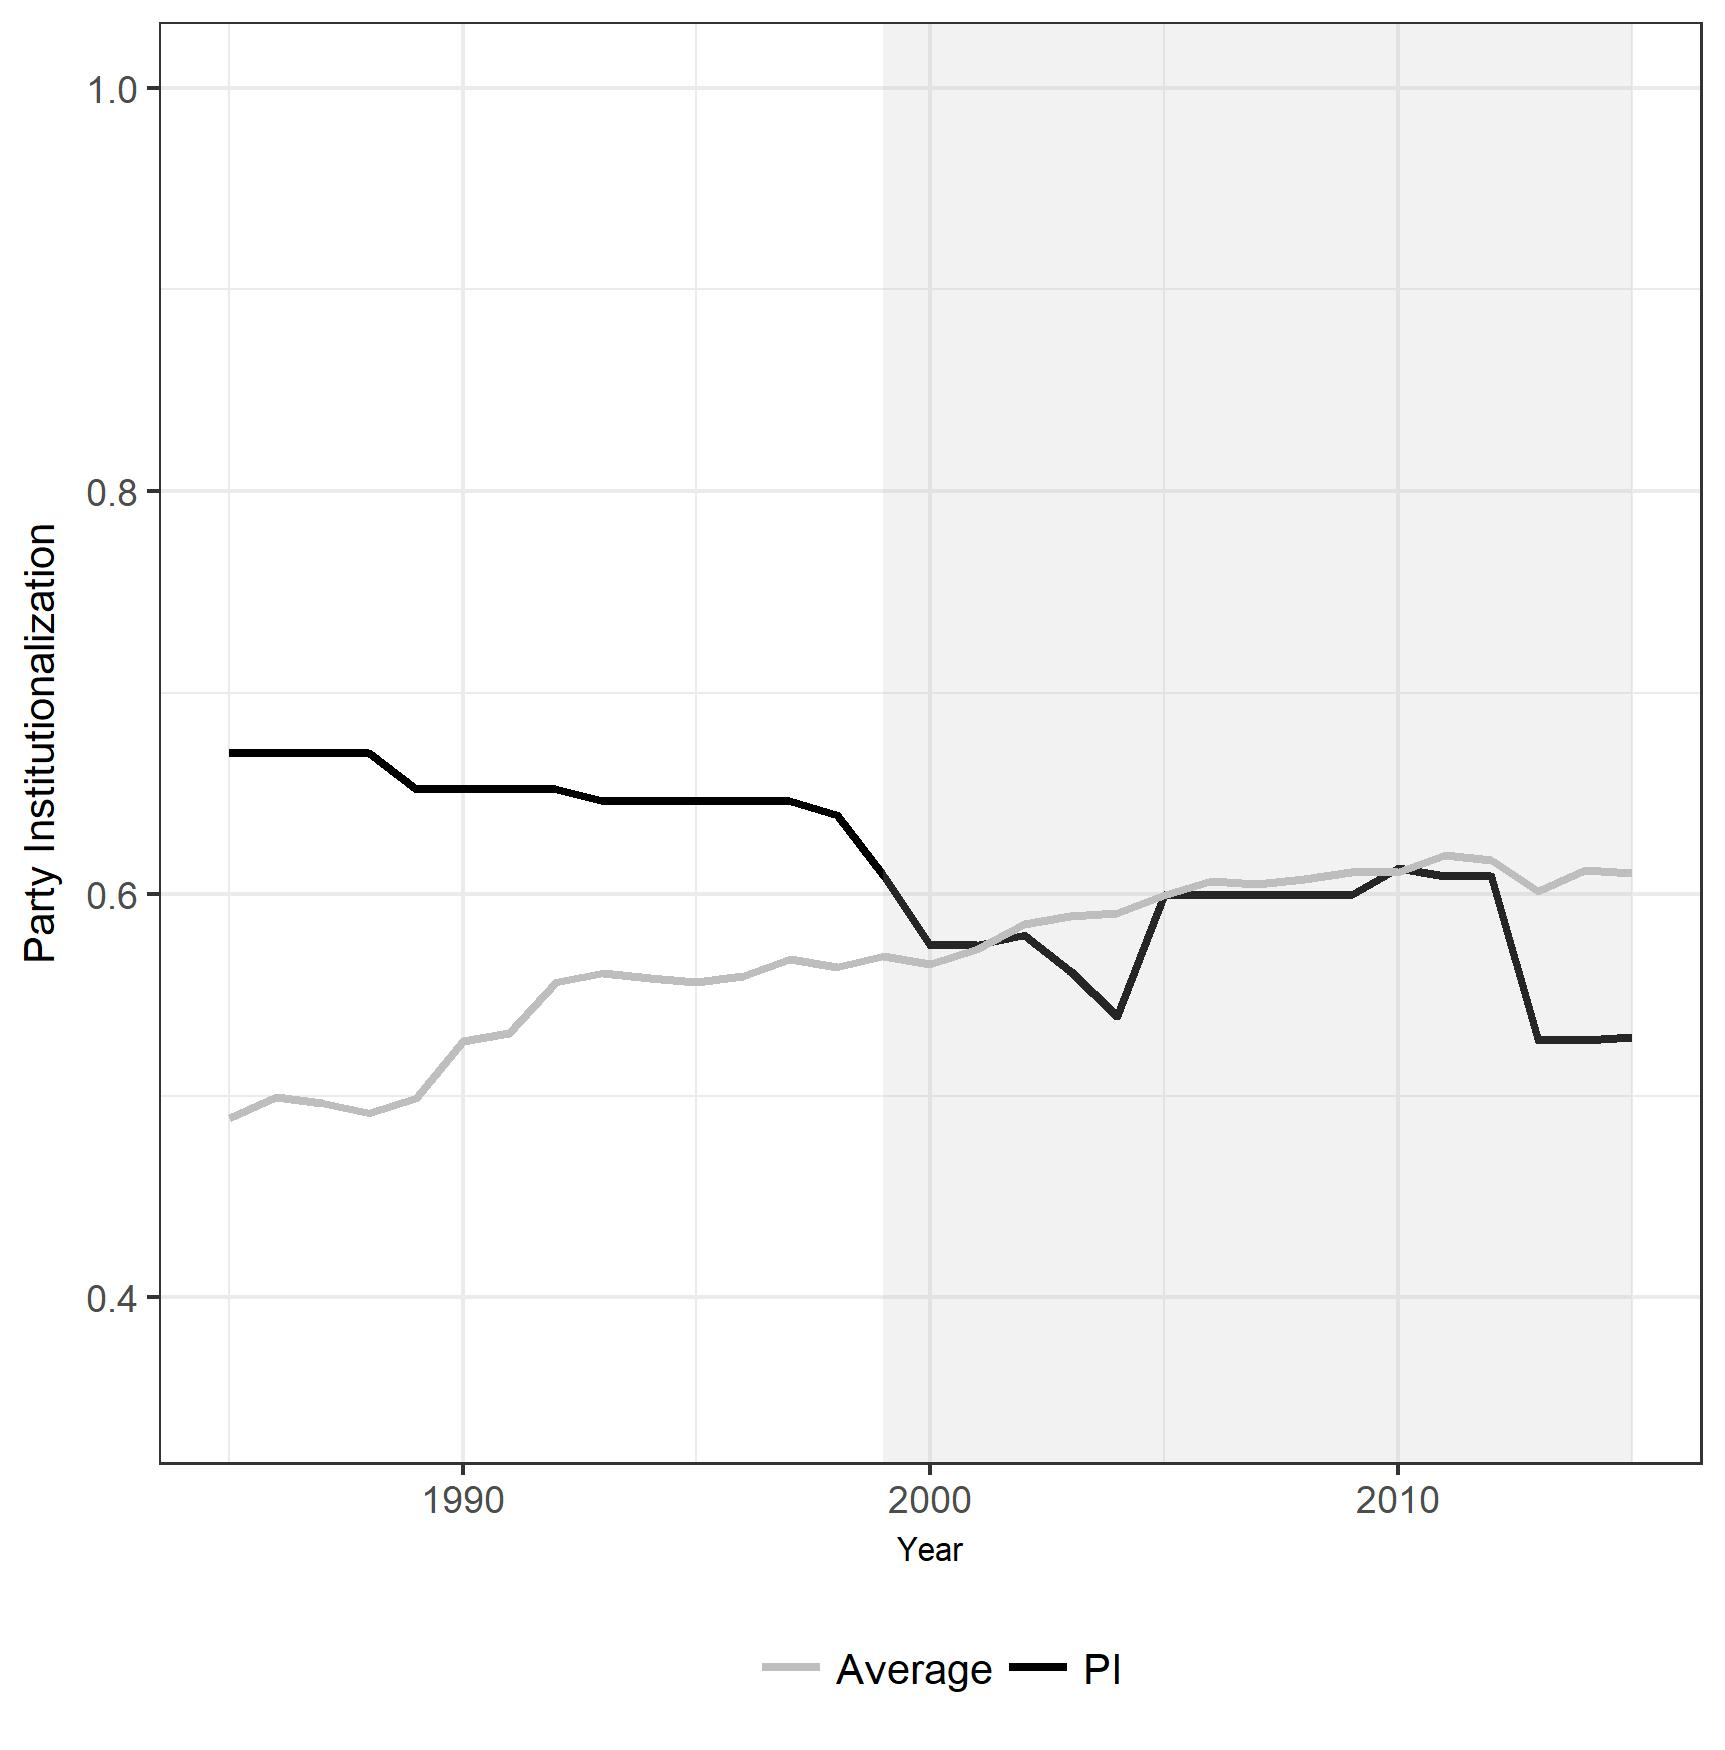
\includegraphics[width=65mm, height=65mm]{venezuela1.jpg}}%
\qquad
\begin{minipage}{2in}%
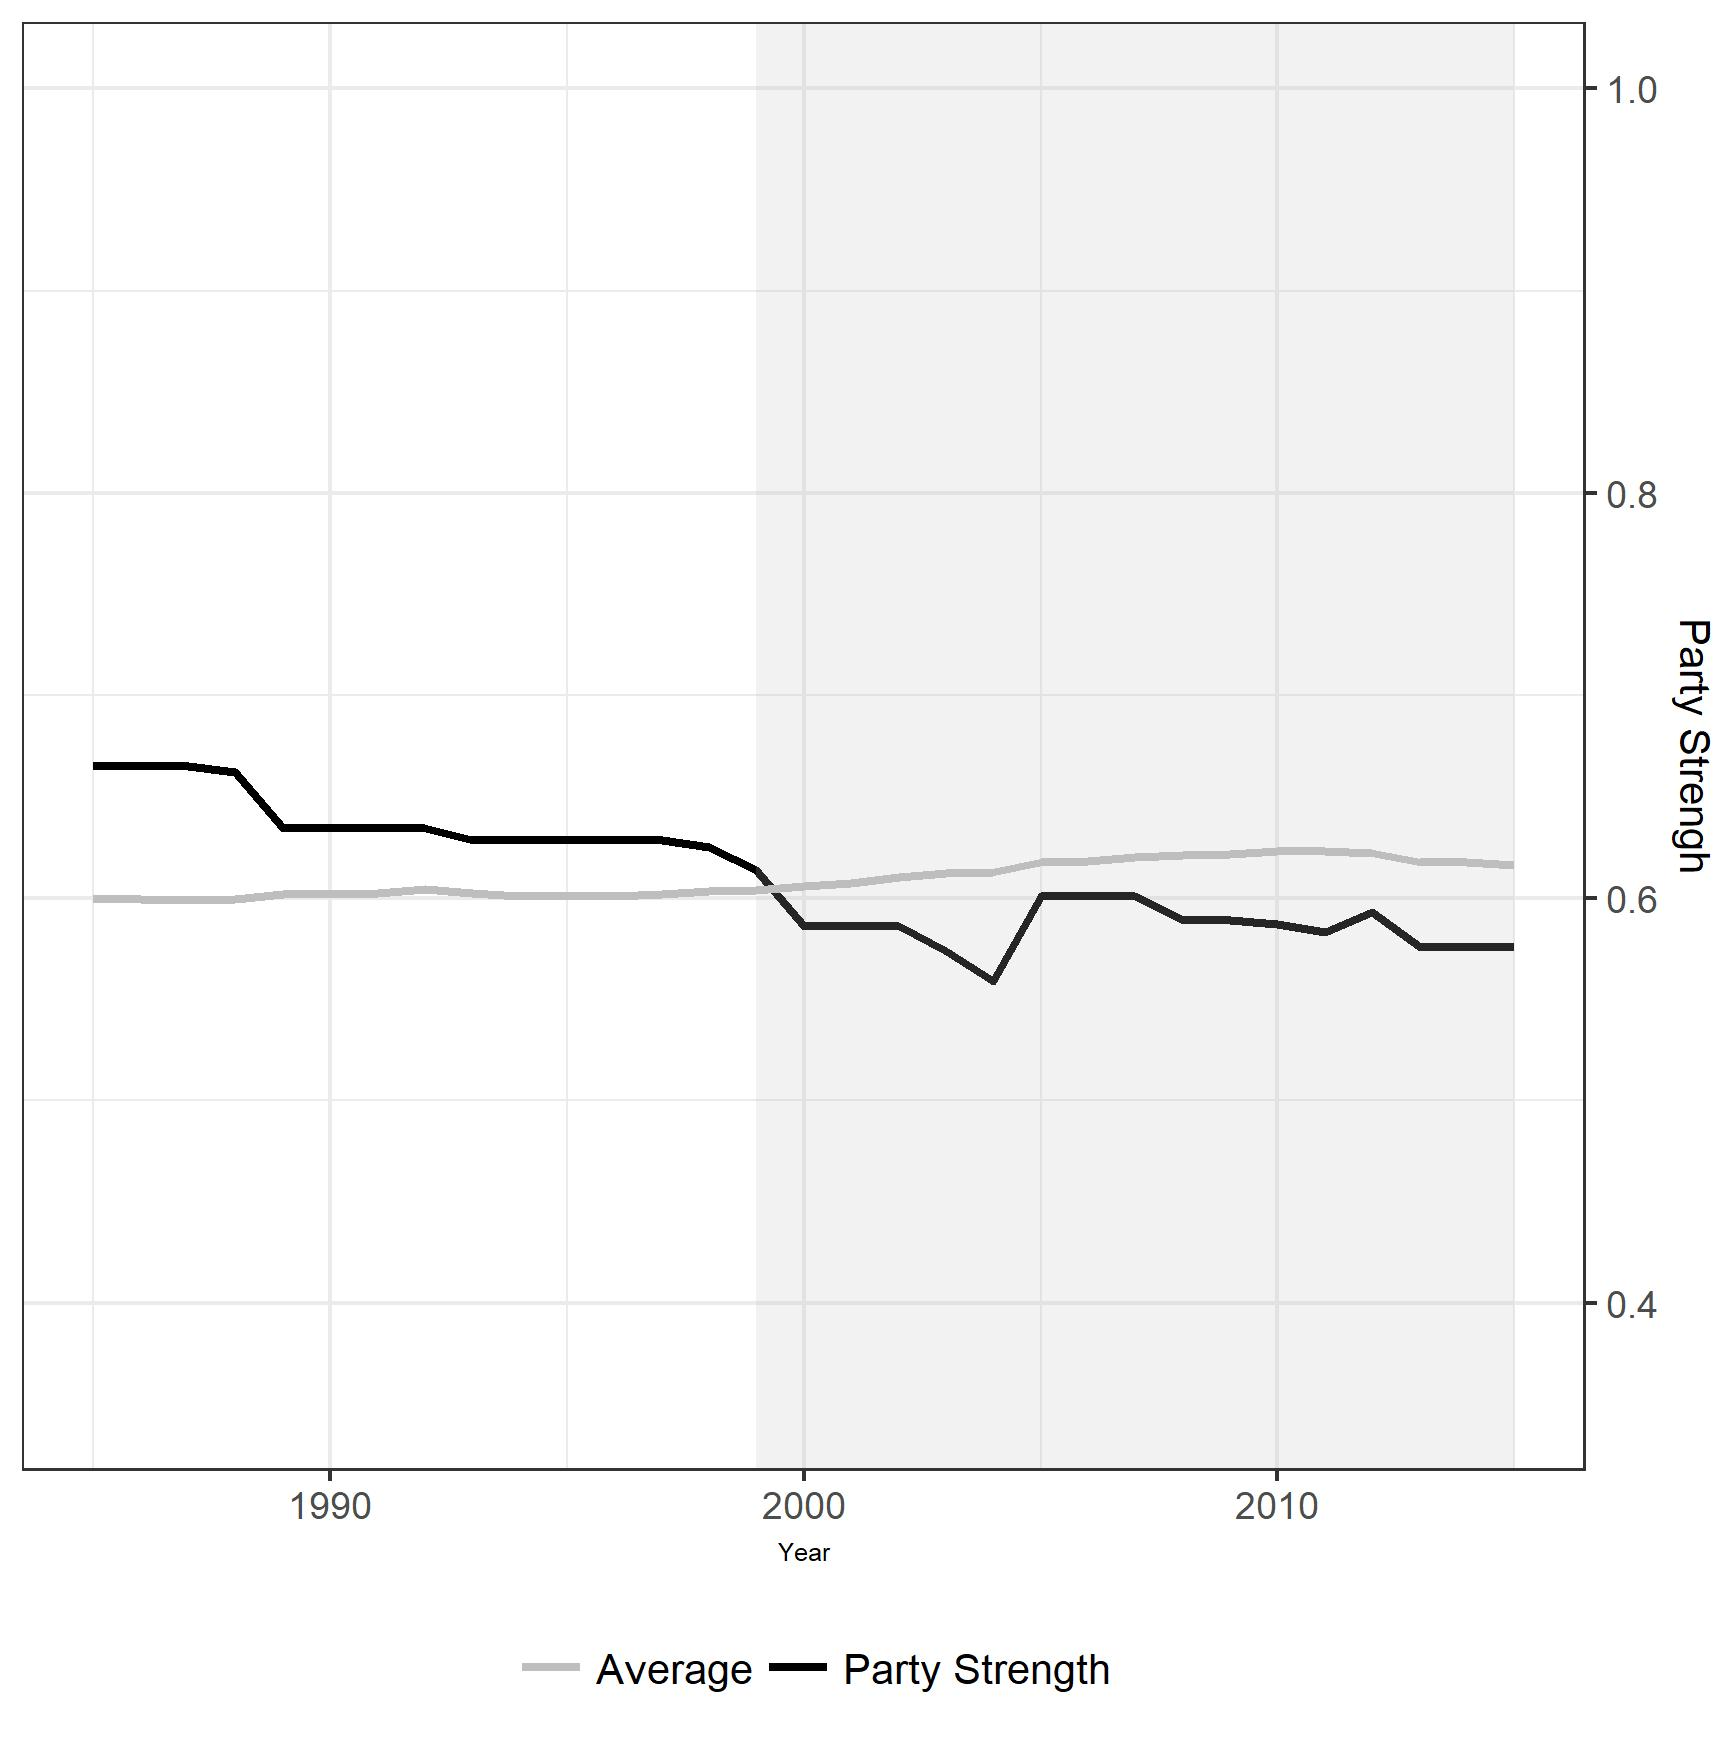
\includegraphics[width=65mm, height=65mm]{venezuela2.jpg}
\end{minipage}%
\caption{Venezuelan Party Institutionalization and Party Strength}%
\label{venezuelapsi}%
\end{figure}
%%%%%%%%%%%%%%%%%%%%%%%%%%%%%%%%%%%%%%%%%%%
\noindent 
\textit{Bolivia} \\
Another participant in Latin America's populist revival \citep{roberts2007latin} is Evo Morales and his \textit{MAS} party in Bolivia. The story of Bolivia's party system is similar to that of Venezuela's. Following years of state-led economic intervention, neo-liberal reforms played a critical role in undermining the foundation upon which political parties rested by significantly weakening organized labor unions \citep{crabtree2013mnr, roberts2013market}. From the mid-1980s, when neo-liberal reforms were first introduced, to Evo Morales' victory in 2006, the electoral and party system in Bolivia was fraught with instability. 
\par
Following the neo-liberal reforms in the mid-1980s politics was characterized by multiple parties and weak coalition governments \citep{crabtree2013mnr}. A new  electoral system introduced in 1995 further contributed to upheaval in the party system \citep{centellas2009electoral}. Overall, net electoral volatility rose from 27.5 from 1980-2000 to 50.7 during 2000-2010 demonstrating the collapse of the Bolivian party system \citep[pg. 1441]{roberts2013market}. Indicative of this instability was the rise of new parties or previously peripheral parties which garnered significant portions of the vote. The presence and success of new or previously peripheral parties is consistent with the low level of institutional hostility in the Bolivian party system which set the stage for the rise of Evo Morales. 
\par
Years before he would ascend to the presidency, Evo Morales rose to prominence as an organizer of coca unions. Following his capture of the previously defunct MAS party, Morales capitalized on opportunities during the Water and Gas Wars to build a larger movement that extended beyond coca growers \citep{webber2011rebellion}. Using a new form of ethno-populism, Morales fused together a new movement-party that cut across multiple ethnicities which had previously acted autonomously. Using populism, Morales was able exploit the weakness in the Bolivian party system and capture power. 
\par
Turning to Figure \ref{boliviapsi} we see that, overall, the Bolivian case fits our expectations for a situation in which populism can succeed. With relatively low levels of party institutionalization and a permissive electoral system new parties were able to enter and contest elections with some success. We also see some evidence, however, that the entrance of the MAS strengthened the fledgling party system. 
     \par
\begin{figure}[H]
\centering
\parbox{2.5in}{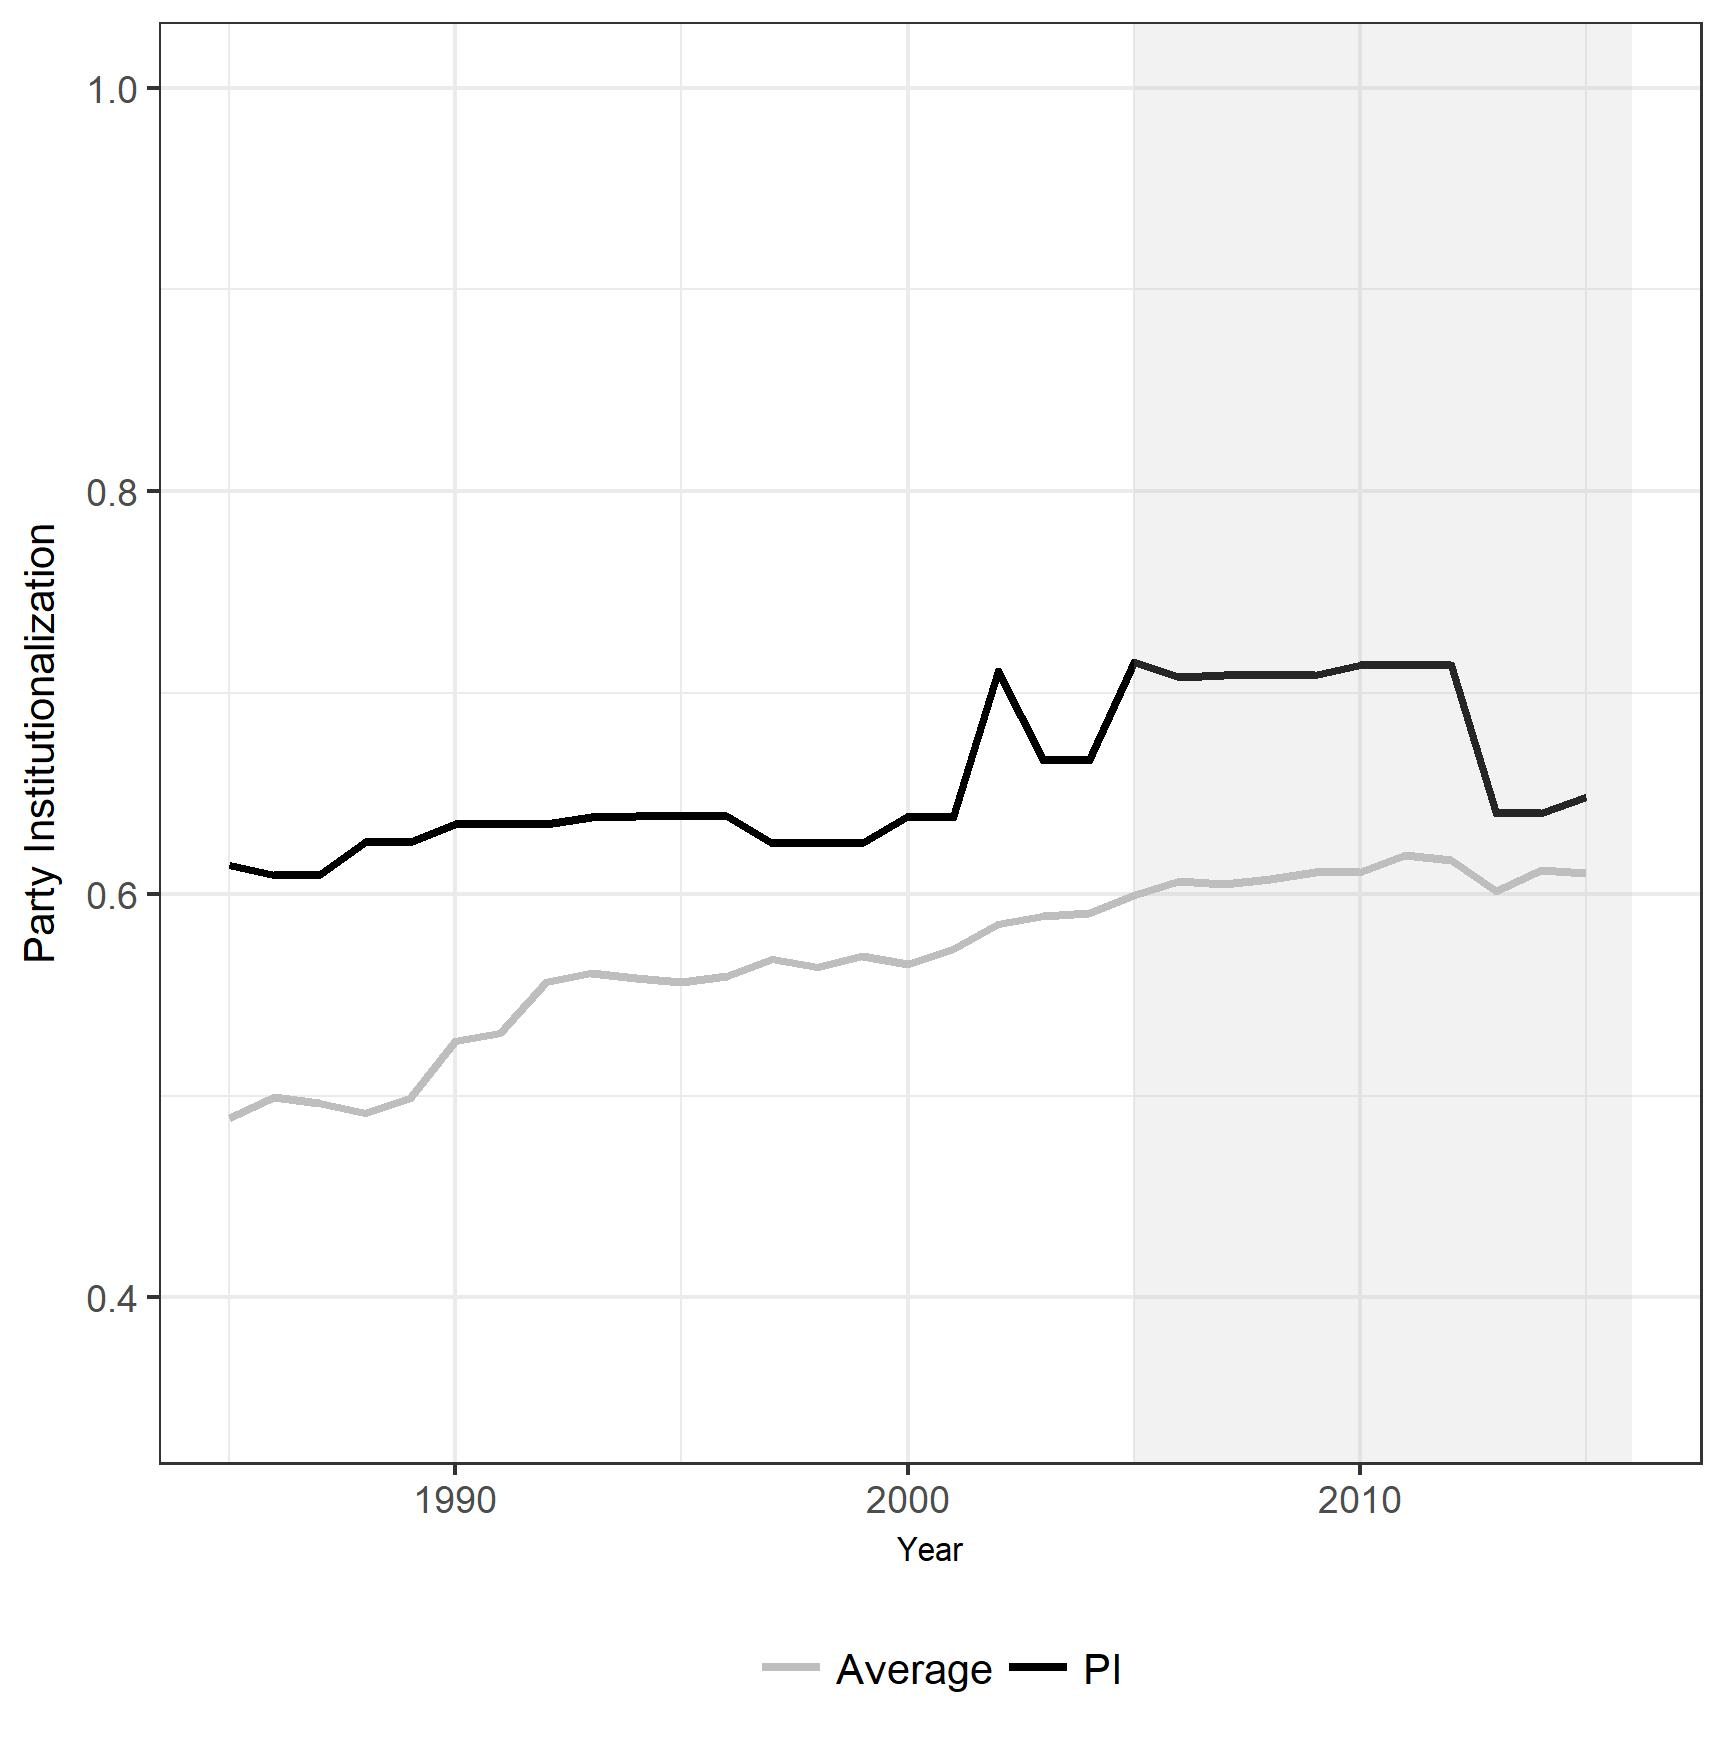
\includegraphics[width=65mm, height=65mm]{bolivia1.jpg}}%
\qquad
\begin{minipage}{2in}%
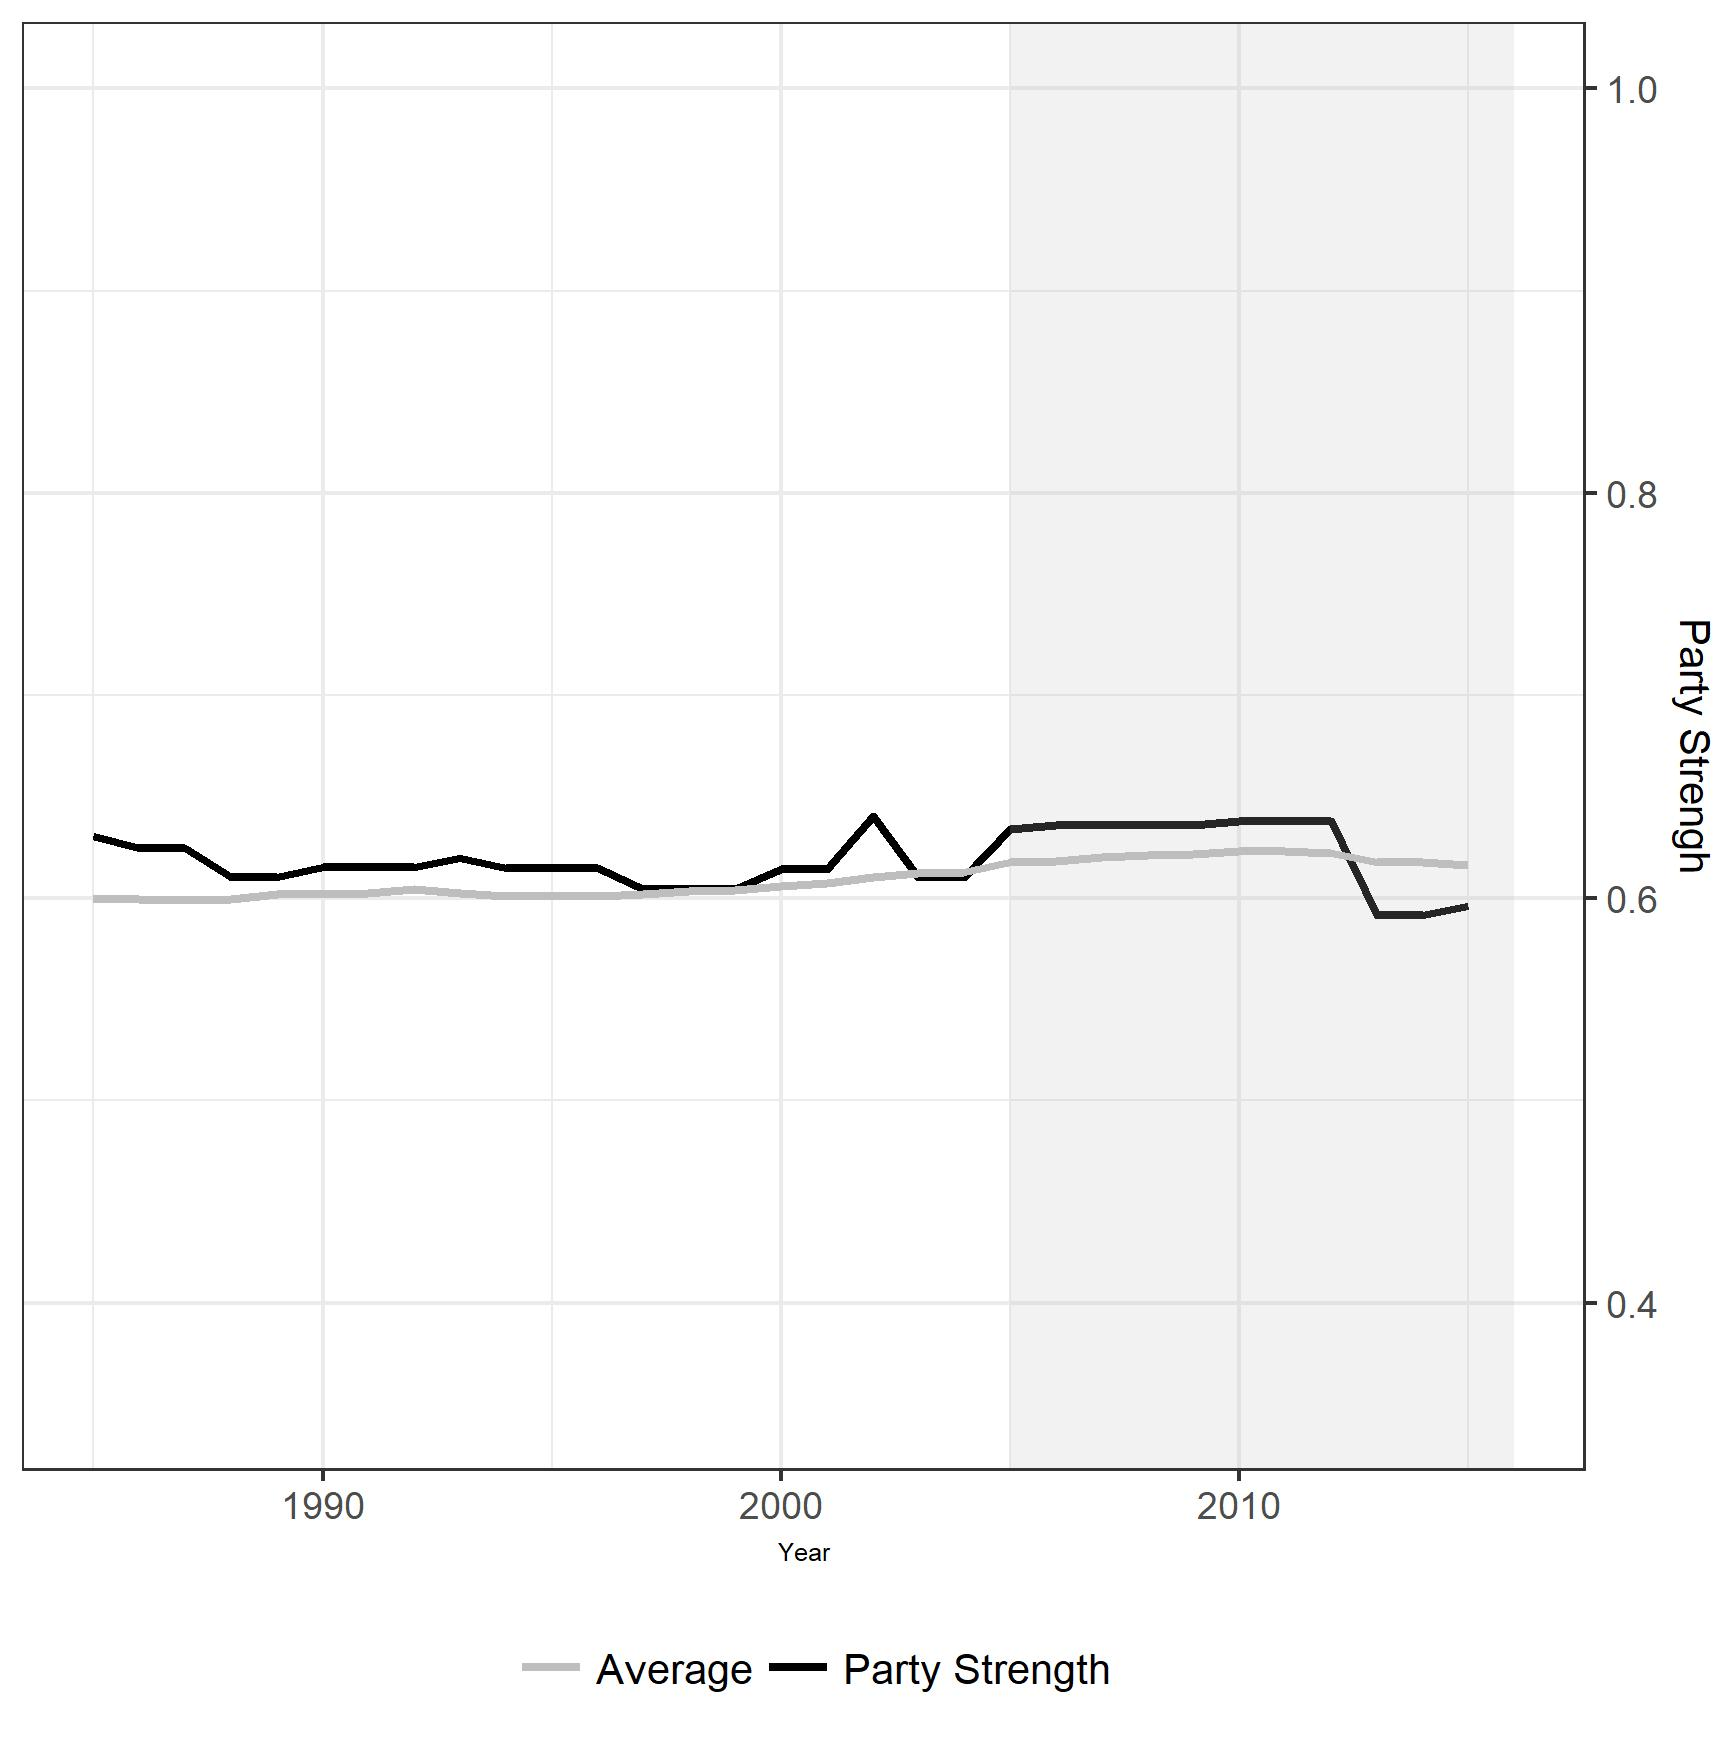
\includegraphics[width=65mm, height=65mm]{bolivia2.jpg}
\end{minipage}%
\caption{Bolivian Party Institutionalization and Party Strength}%
\label{boliviapsi}%

\end{figure}
%\FloatBarrier
%%%%%%%%%%%%%%%%%%%%%%%%%%%%%%%%%%%%%%%%%%%%
  \noindent 
\textit{Spain} \\
Both the Bolivian and Venezuelan party systems are near or below the global average. By contrast, party systems in  Europe are relatively well-institutionalized. To what extent do we observe populist competition in systems where parties are better institutionalized? The case of Spain demonstrates that populists can compete and have some success where the electoral system is sufficiently permissive. Figure \ref{spainpsi} shows that both \textit{PI} and \textit{Party Strength} are well above the global democratic average. Following the merger of parties that created the PP (\textit{Partido Popular}) Spain has been a fairly stable two-party system with the PP and PSOE (\textit{Partido Socialista Obrero Espa\~{n}ol}) garnering a strong majority of the vote even with a fairly permissive electoral system. Following a reform of the electoral system in 1985 both the PP and PSOE garnered sufficient electoral support to maintain a two-party system despite Spain's use of multi-member district proportional representation and a fairly large district magnitude of 6.73 \citep{selway2016system}.
\begin{figure}%
\centering
\parbox{2.5in}{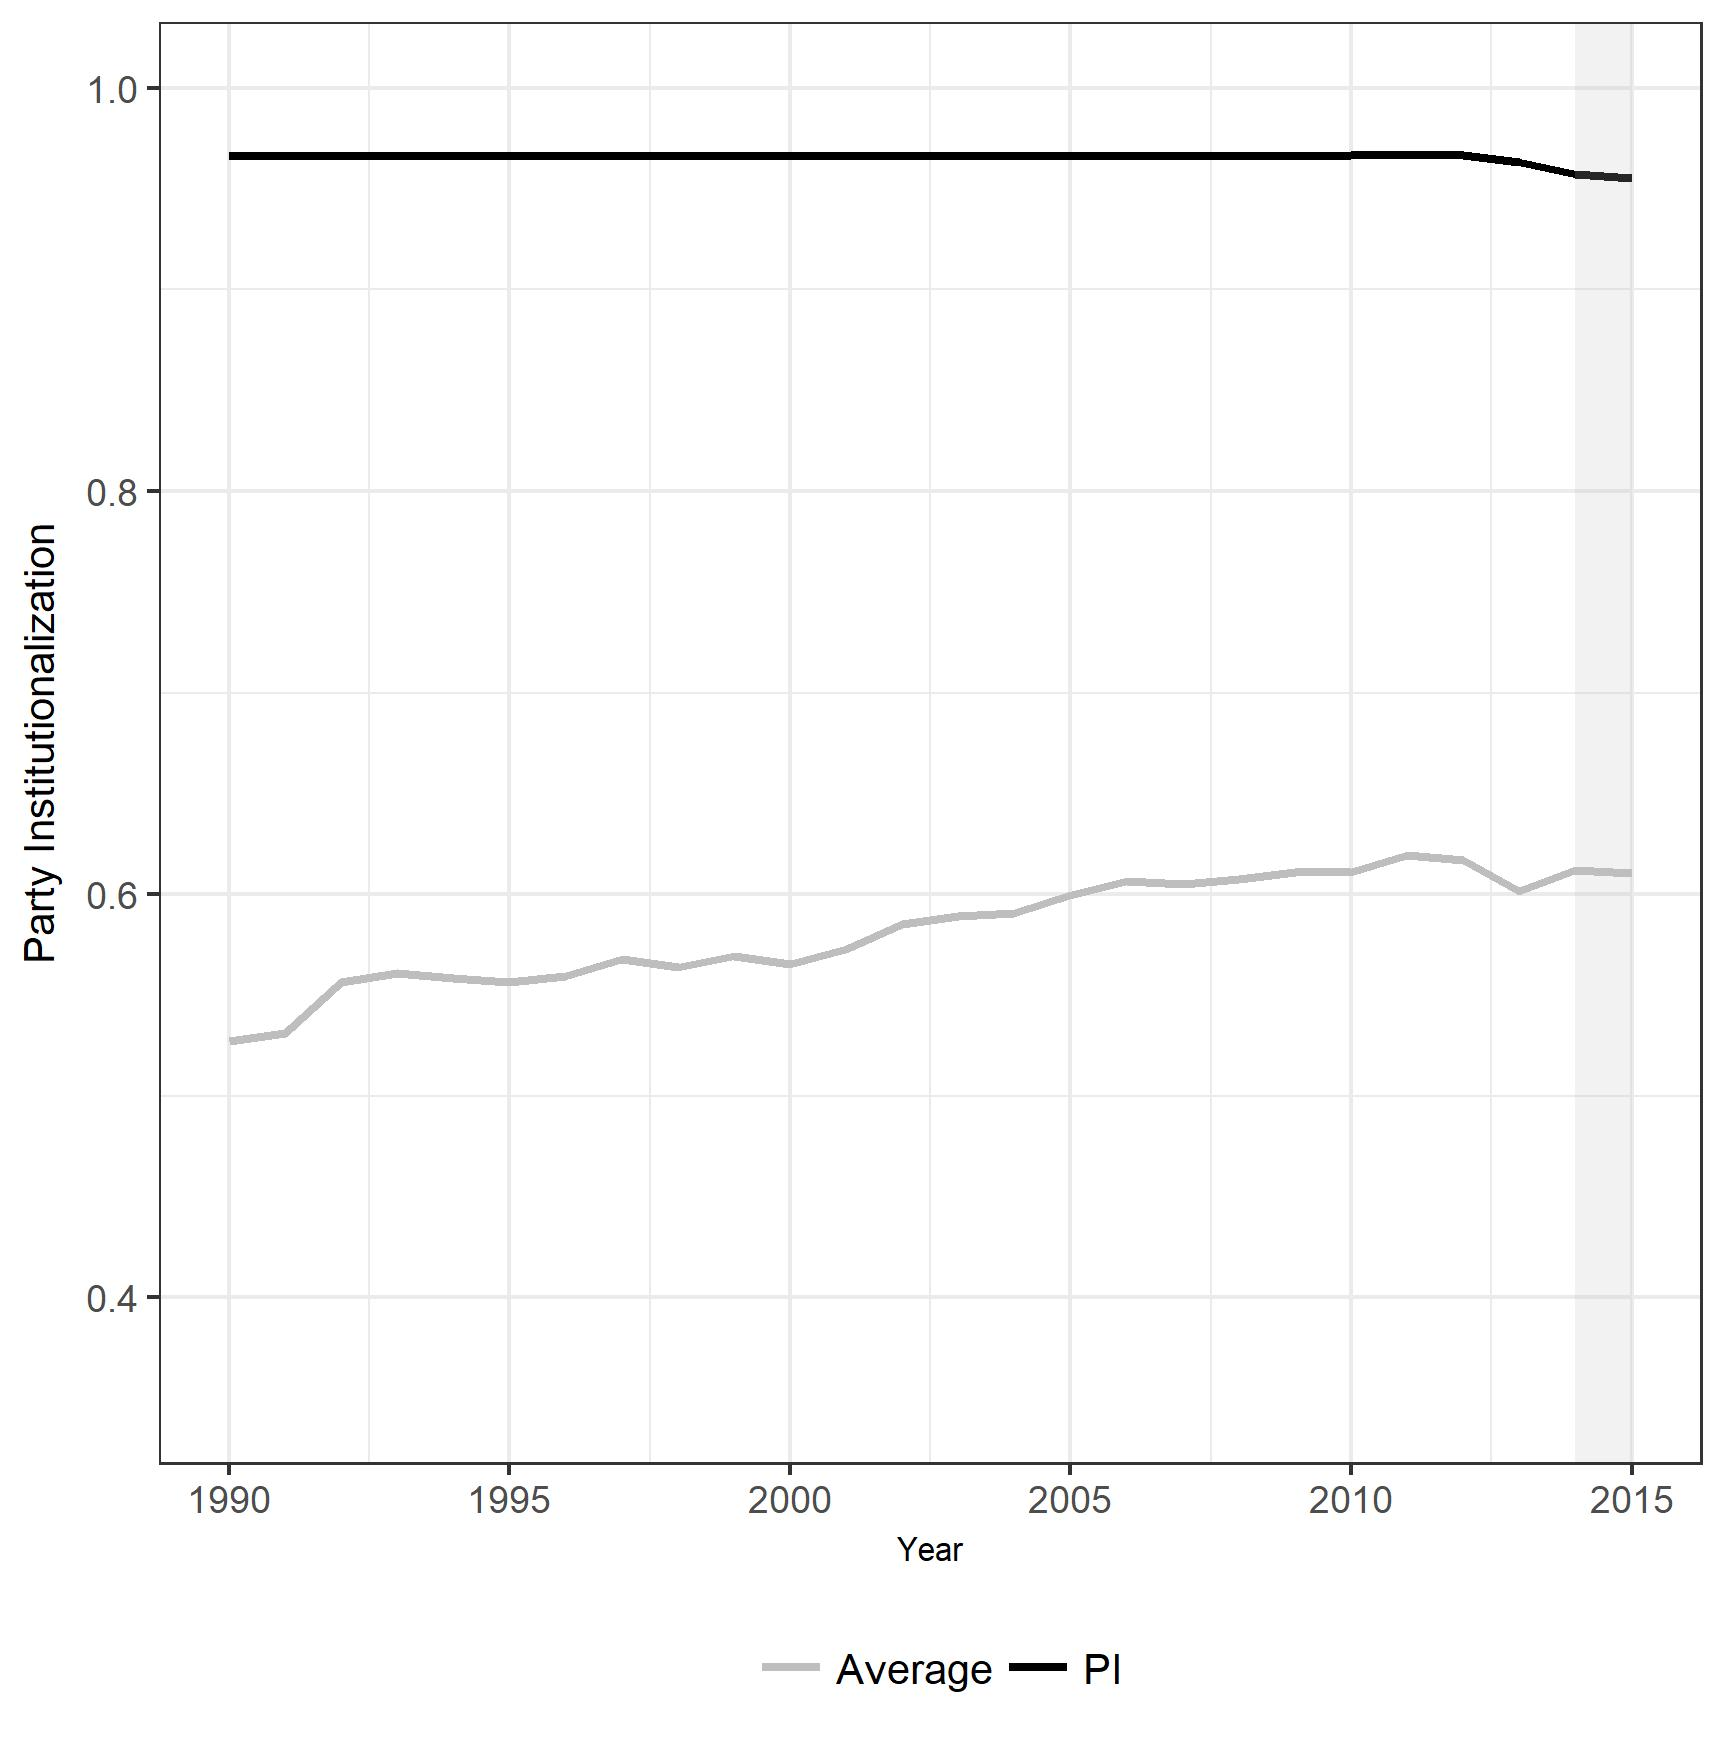
\includegraphics[width=65mm, height=65mm]{spain1.jpg}}%
\qquad
\begin{minipage}{2in}%
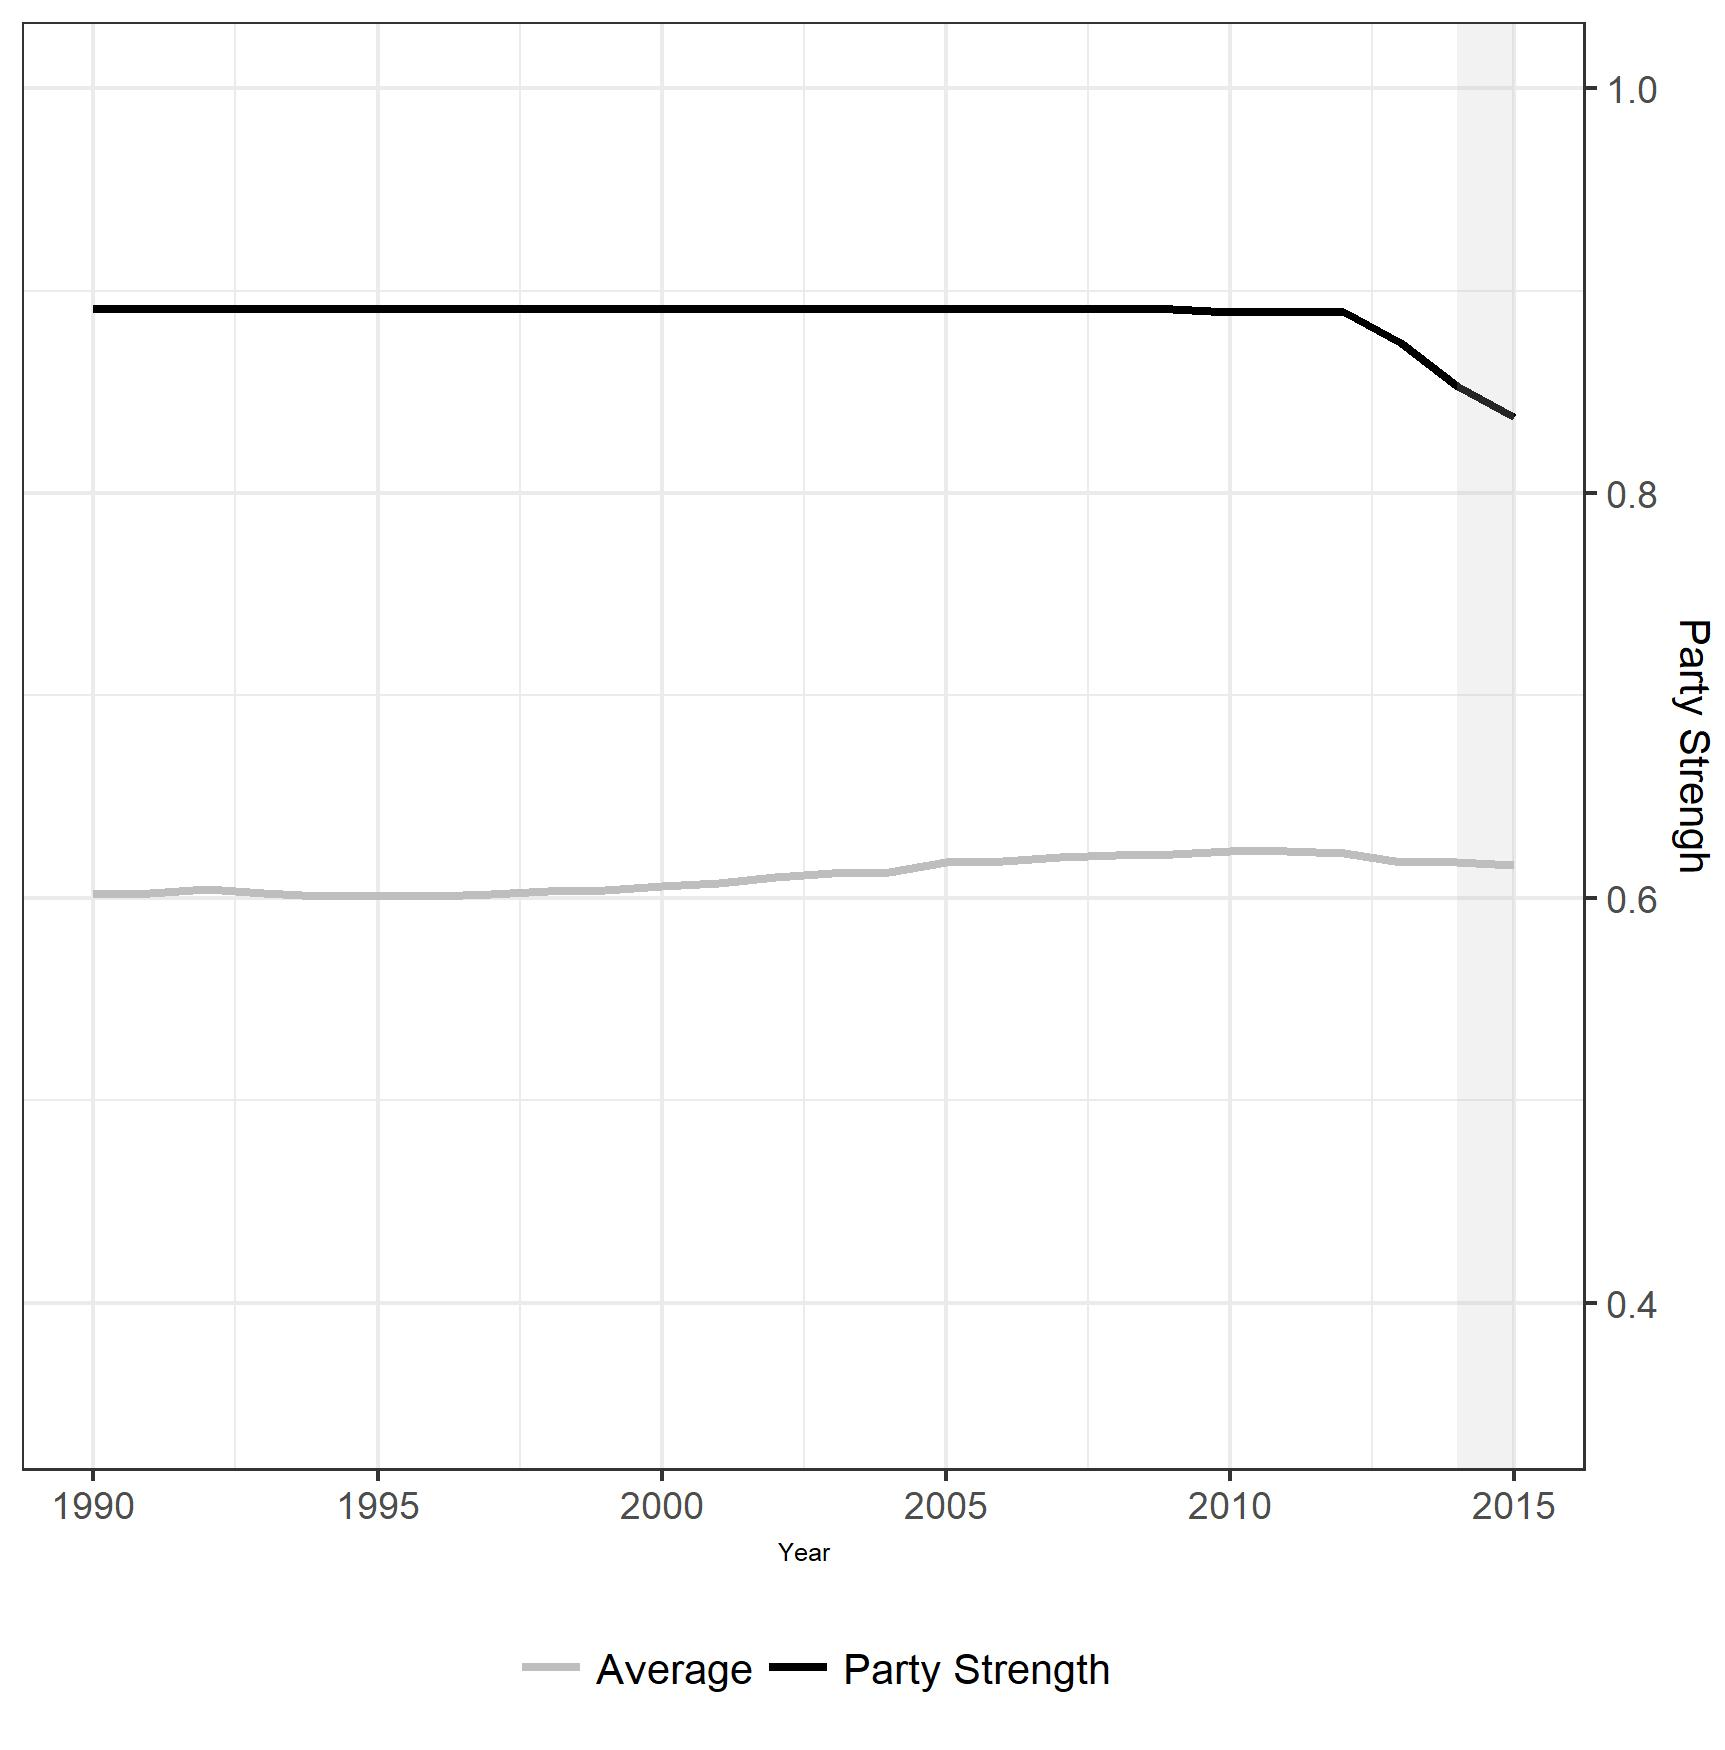
\includegraphics[width=65mm, height=65mm]{spain2.jpg}
\end{minipage}%
\caption{Spanish Party Institutionalization and Party Strength}%
\label{spainpsi}%
\end{figure}
\par
The conditions in Spain since the 2008 global financial crisis were similar to those that led to the rise of successful populists in Bolivia and Venezuela. Following the financial crisis, unemployment rose steadily to an extremely high level (Figure \ref{spain_unem}). Yet this large and persistent economic malaise didn't immediately lead to any breakdown in the Spanish party system. Instability only began after the center-left PSOE agreed to austerity measures. Like other cases of populism in Latin America, the act of a leftist party agreeing to austerity measures was a bait-and-switch tactic with the potential to programmatically de-align the party with many of its followers \citep{roberts2013market}. In fact, following the PSOE's introduction of austerity measures a large-scale protest broke out across the country and the party was eventually dealt a major blow, losing 15\% of the vote from the previous election. However, despite the magnitude of the protests and the electoral defeat of the PSOE, the two-party system initially stayed intact with no new parties challenging the PP or PSOE in 2011. 
\par
\begin{figure}%
\centering
\parbox{4in}{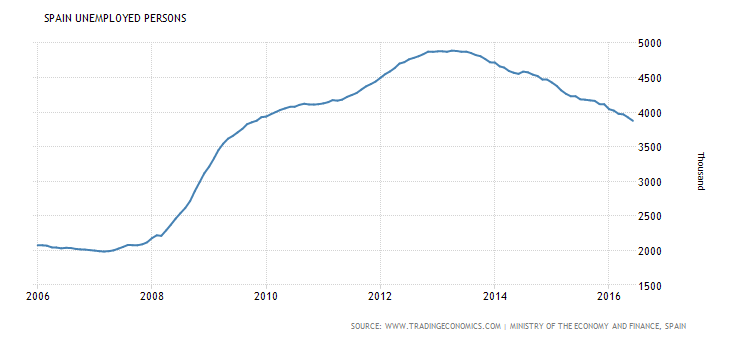
\includegraphics[width=100mm]{spain_unem.png}}%
\caption{Spanish Unemployment (2006-2016)}%
\label{spain_unem}%
\end{figure}
Despite the electoral hold PSOE and PP maintained, the links between voters and the existing parties had been weakened as a result of the sustained economic crisis and the government responses to it. Figure \ref{spainpsi} picks up this change, as \textit{PI} and Party Strength decrease sprior to the 2015 election. As the level of institutionalization declined, the permissive electoral system allowed for the entry of new competitors. In both the local and national elections of 2015, two new parties rose to prominence one of which, Podemos, is very populist. 
\par
Given the political fragmentation after the 2015 election the parties were unable to form a government and new elections were held in mid-2016. As can be seen in Table \ref{spainvotes} the electoral fortunes of the new parties' (Podemos and Ciudadanos), as well as PSOE, were largely unchanged, while the center-right PP made modest gains. Spain demonstrates how populist parties can enter into what had been a well institutionalized system. Following sustained and fairly extreme economic duress \textit{and} a shift by the ruling party away from their programmatic alignment with their voting base, space opened for Spanish populists. 

%%%%%%%%%%%%%%%%%%%%%%%%%%%%%%%%%%%%%%%%%%
\begin{table}[!htbp]
\centering 

  \caption{Elections Results in Spain (2011-2016)} 
  \label{spainvotes} 

\begin{tabular}{@{\extracolsep{5pt}} cccc} 

\hline \\[-5ex] \\
Party & 2011 & 2015 & 2016 \\ 
\hline \\[-5ex] \\
PSOE & 28.76 & 22.00 & 22.66 \\ 
PP & 44.63 & 28.71 & 33.03 \\ 
Podemos+ & NA & 20.68 & 21.15 \\ 
Cs & NA & 13.94 & 13.06 \\ 
\hline \\[-1.8ex] 
\end{tabular} 

\end{table}
%%%%%%%%%%%%%%%%%%%%%%%%%%%%%%%%%%%%%%%%%%
\par
In that less-institutionalized environment Spain's permissive electoral rules opened the door for a new populist party to enter. However, the high level of party institutionalization presents challenges for this new populist party. It remains to be seen whether Podemos can rely heavily on strong populist rhetoric to compete with institutionalized parties. According to our theory the (still) high level of \textit{PI} and \textit{Party Strength} stand as an obstacle to Podemos' future success. 



%%%%%%%%%%%%%%%%%%%%%%%
\subsection*{Populist Targeting and Adaptation}
%%%%%%%%%%%%%%%%%%%%%
\noindent
\textit{Austria} \\
To demonstrate how institutional hostility dampens the presence of populism in a party system we have selected the case of the  FP\"{O}  in Austria – one of the most notable cases of populism in Europe today. The FP\"{O} was founded in 1956 by former members of the Nazi party but was a minor party for most of its early life. The fortunes of the FP\"{O} changed during the 1980s following a change in leadership. In 1986 J\"{o}rg Haider became chairman of the FP\"{O} and quickly changed course. In an attempt to broaden the appeal of the FP\"{O}, J\"{o}rg Haider abandoned the previous agenda and retooled the party with a populist-nationalist blend which included a move to the right and strong anti-immigrant sentiment. 

\begin{figure}[H]%
\centering
\parbox{2.5in}{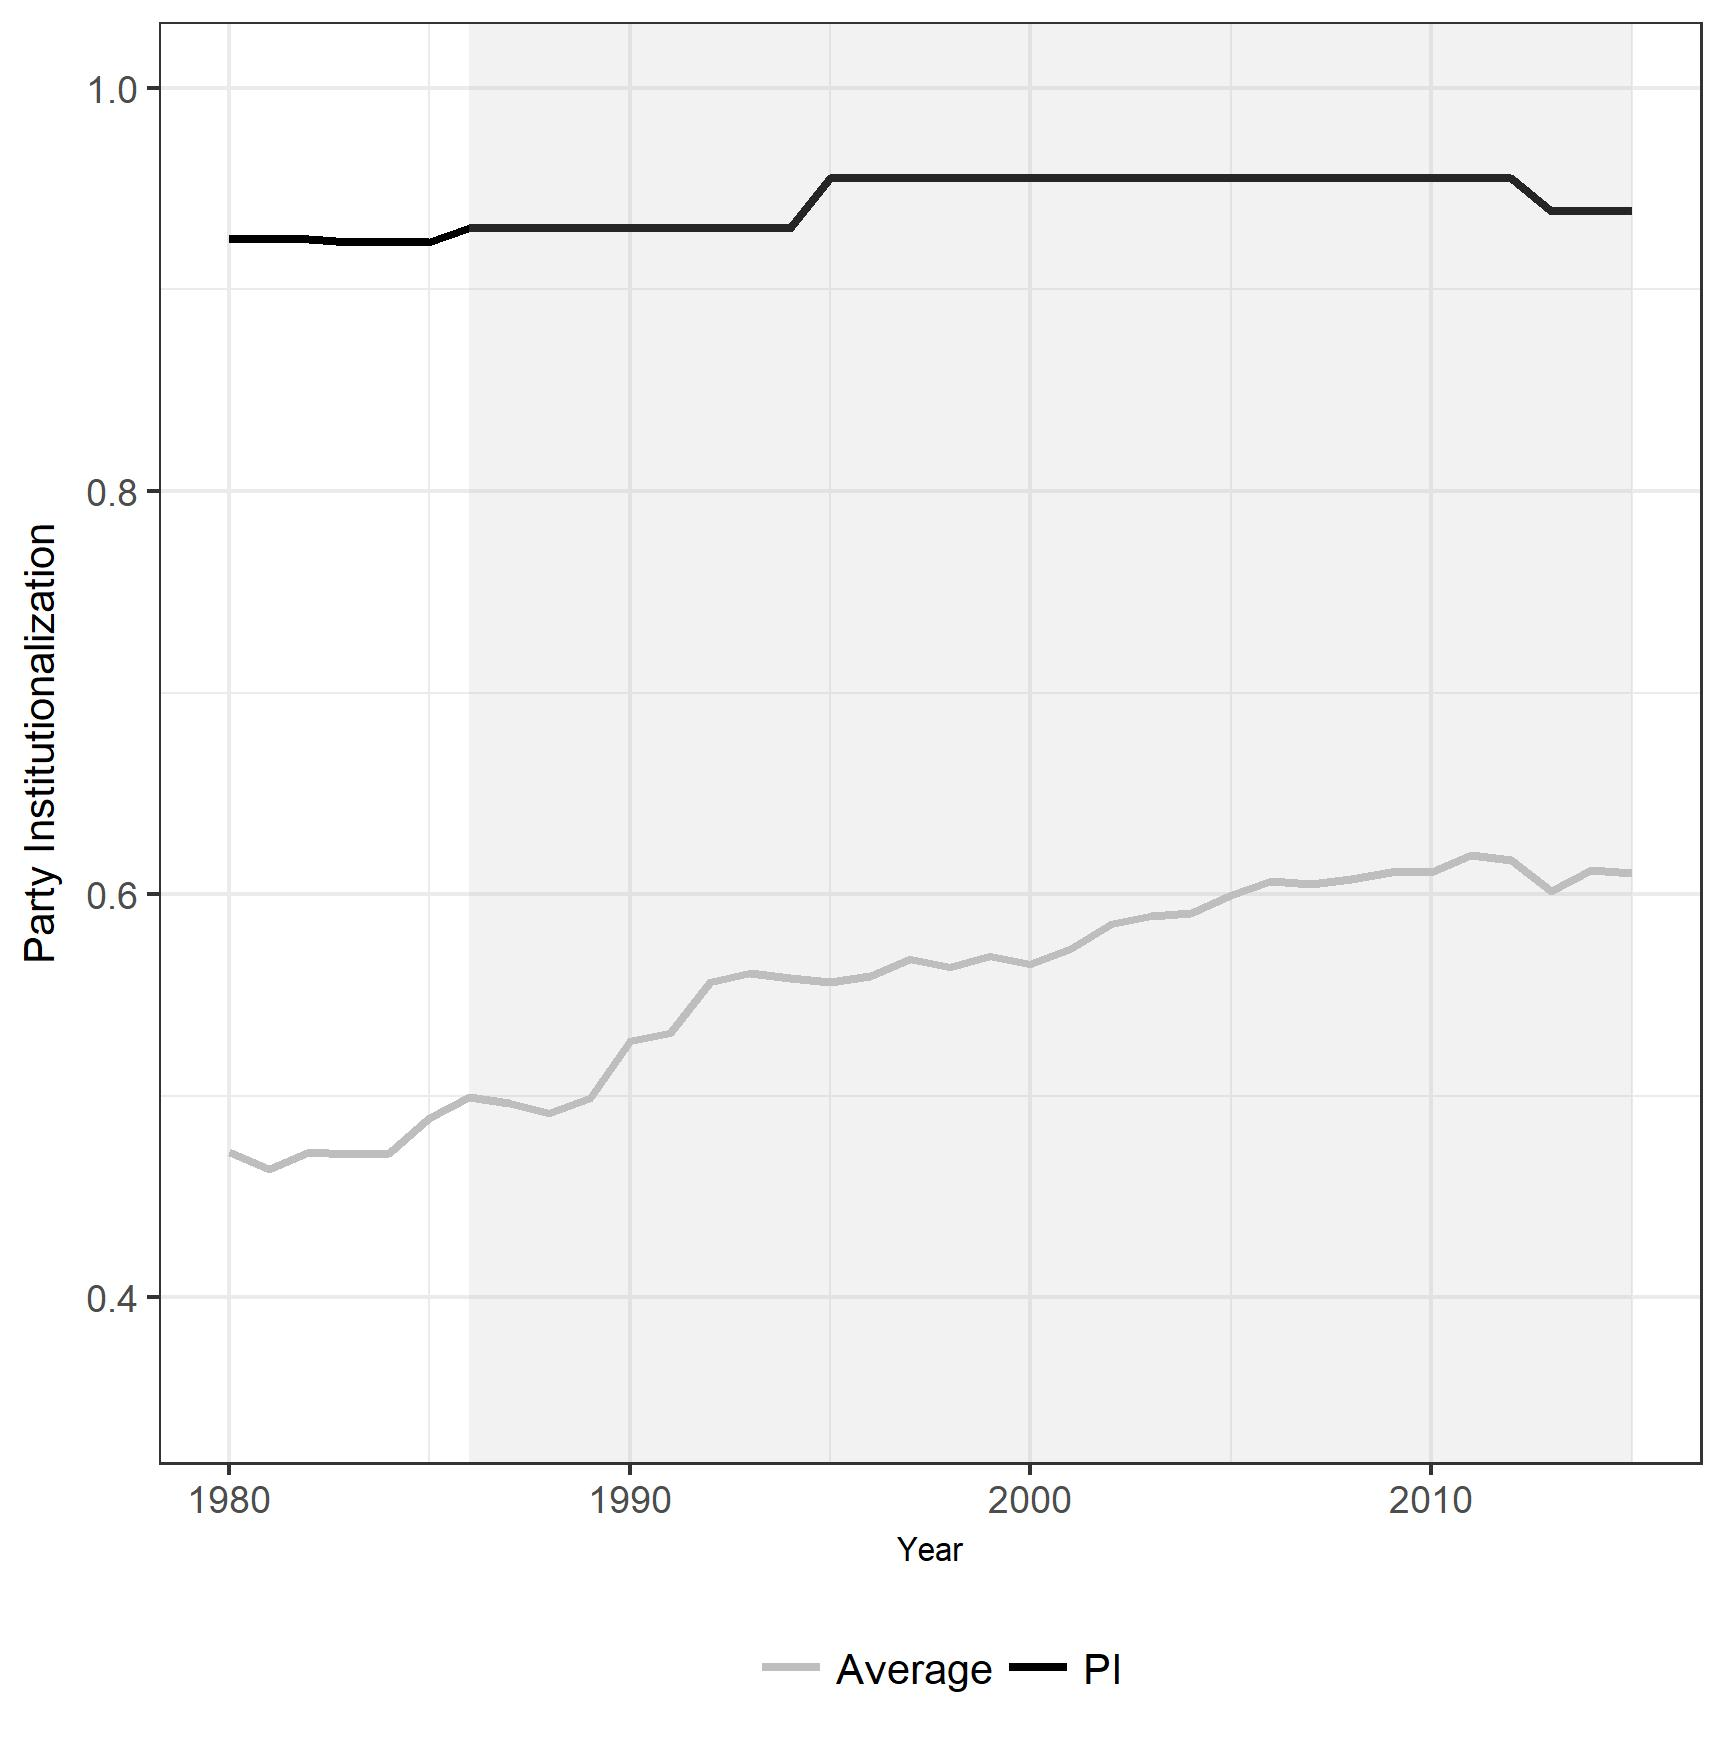
\includegraphics[width=65mm, height=65mm]{austria1.jpg}}%
\qquad
\begin{minipage}{2in}%
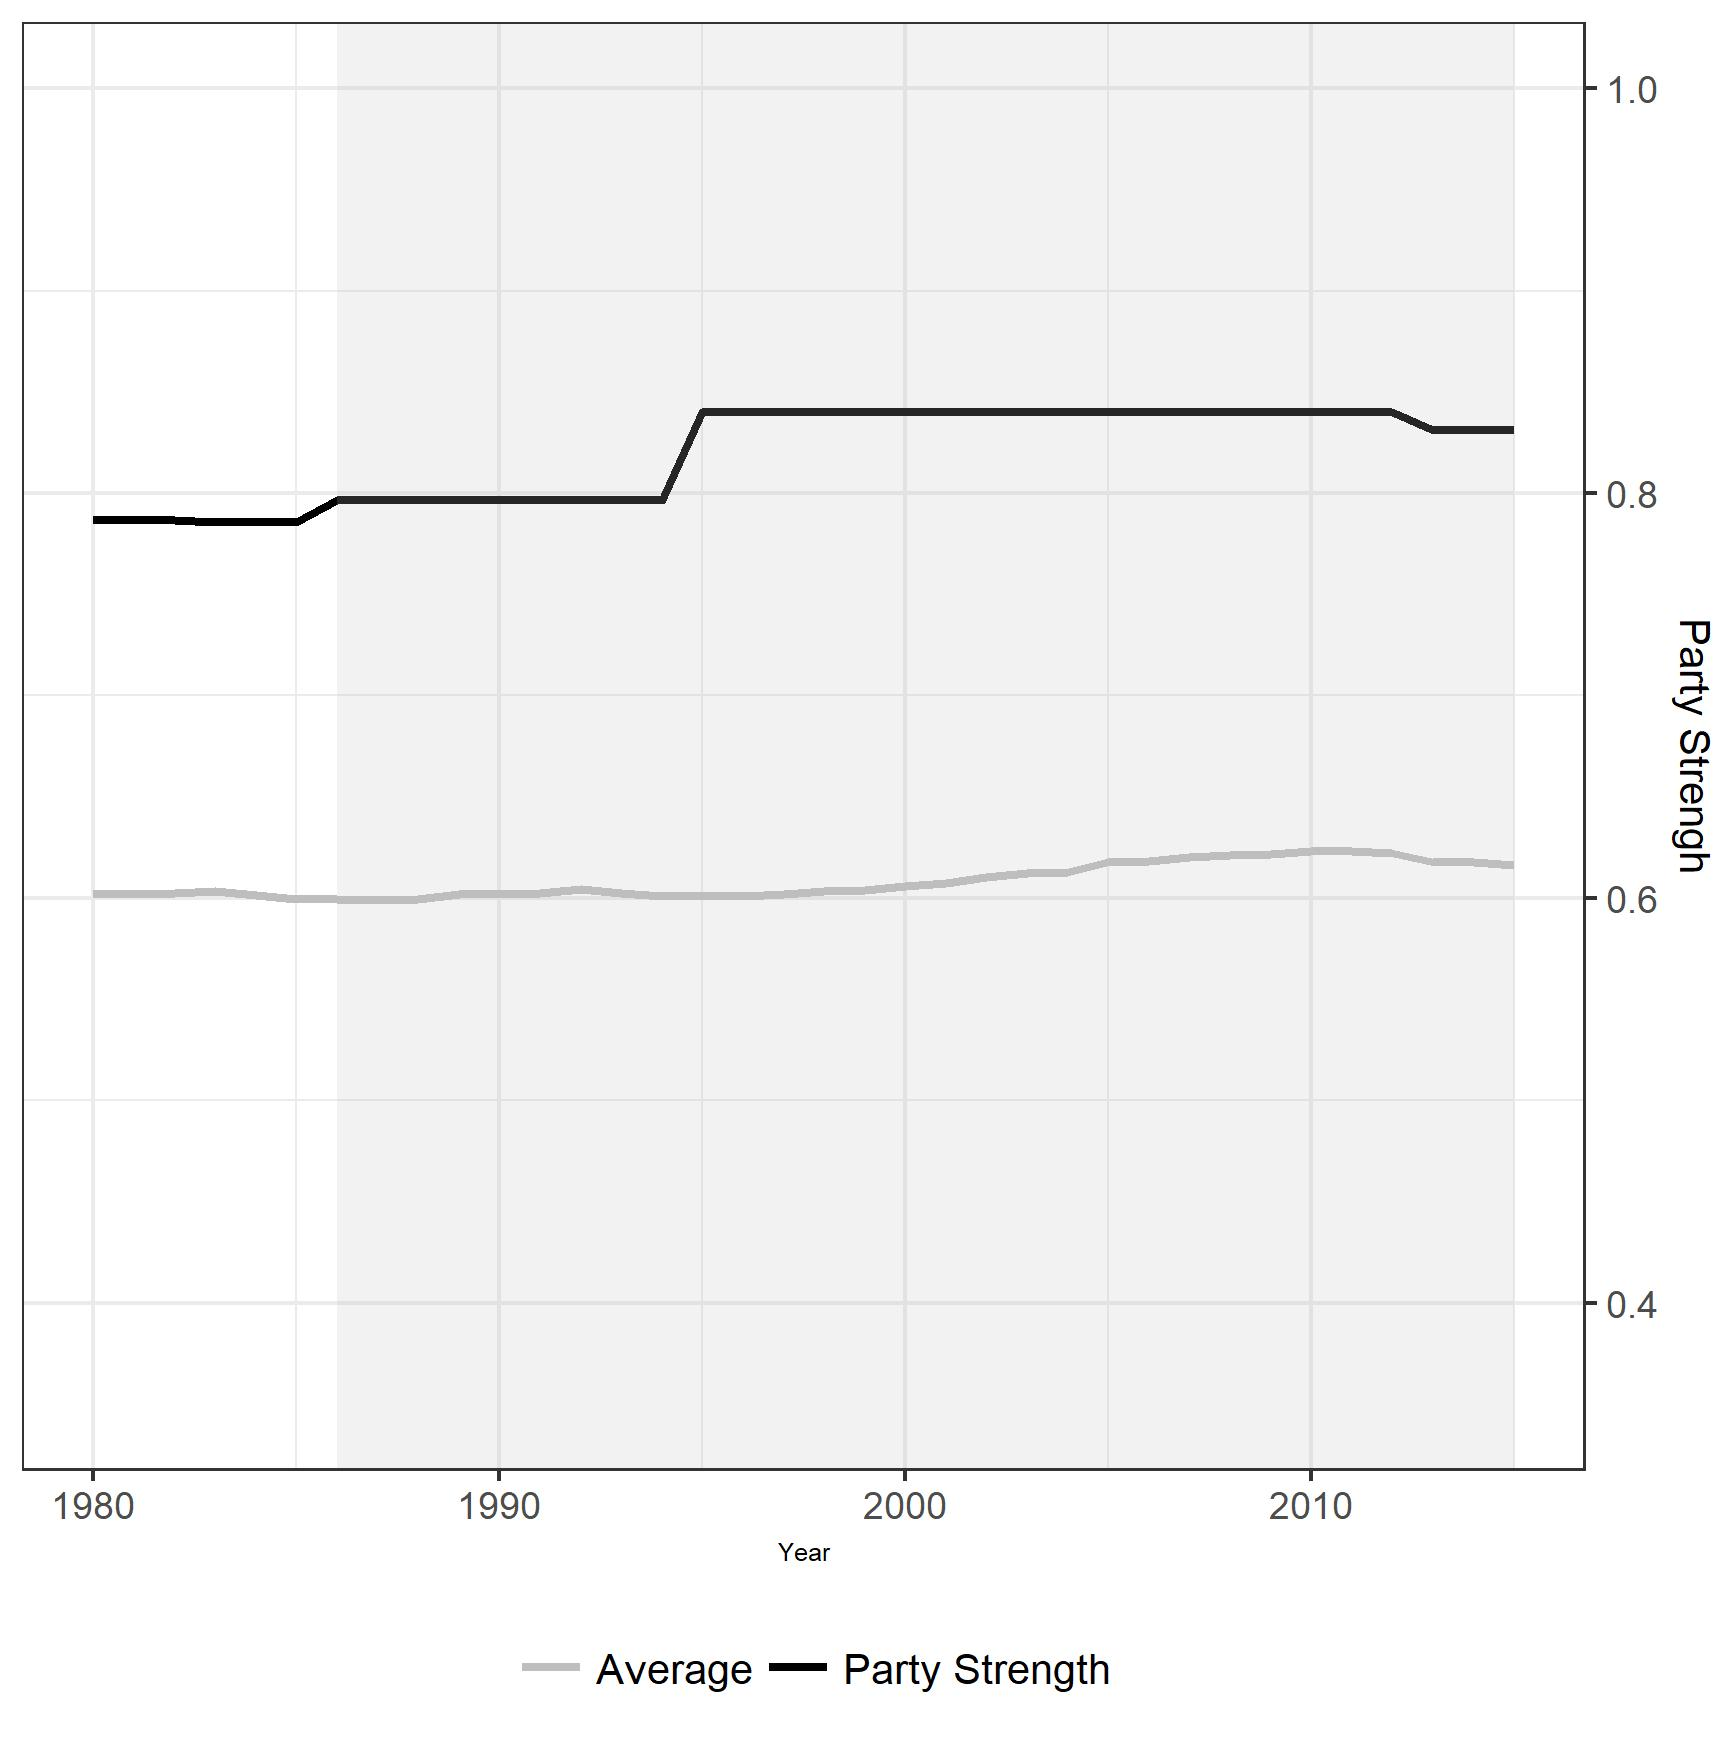
\includegraphics[width=65mm, height=65mm]{austria2.jpg}
\end{minipage}%
\caption{Austrian Party Institutionalization and Party Strength}%
\label{austriapsi}%
\end{figure}
\par
Somewhat surprisingly the move to a populist-nationalist approach in order to broaden the appeal of the FP\"{O} seemed to pay off. In the years following J\"{o}rg Haider's ascendancy in the party, the FP\"{O} started to make inroads within a highly permissive system that had been previously dominated by two parties. Unlike the case in France, the move to a populist strategy was successful because of lower levels of institutional hostility in the Austrian system. Even though the Austrian party system boasted two major and well institutionalized political parties (the SP\"{O} and the \"{O}VP), the nature of Austria's electoral system reduces institutional hostility. As in Spain, the presence of proportional representation in Austria reduces the pressure towards a two-party system and allows greater space for additional parties. In the case of the FP\"{O}, J\"{o}rg Haider was able to find space in the electoral market by using a more expansive appeal with populism. In this way lower institutional hostility, due to permissive electoral institutions, has allowed the FP\"{O} to become a major party (moving from approximately 5\% of the vote to gaining 20.5\% of the vote in 2013 National Council election and 46.2\% in the 2016 Presidential elections). 
\par
The success of the FP\"{O} is also a prime example of populist adaptation. Given the permissive electoral system, populist parties were able to gain an early foothold in the party system. However, the presence of highly institutionalized parties limited the number of voters available for mobilization, relegating the FP\"{O} to minor party status. Two things had to change in order for the party to broaden its appeal. First, a decline in party loyalty over the 1970s and 1980s--not fully captured in our \textit{PI} and \textit{Party Strength} measures, but well documented in the broader literature\footnote{See \citet{muller1993after} for a review of this literature.} --provided a set of unattached/weakly attached voters that new parties could target. Second, the FP\"{O} had to adapt its rhetoric to appeal to a broader set of voters. Over the course of the 1980s the FP\"{O} broadened and moderated its rhetoric. While the FP\"{O} certainly employs populist rhetoric, that rhetoric is less populist than many populist parties in other cases -- it falls at the midpoint in the index of populism created by \textbf{HS}, and well below more radical populist parties such as the PVV in the Netherlands or the NPD in Germany. This adaptation in a moderately hostile environment has allowed the FP\"{O} to grow and become a major party in the system. However, the continued presence of relatively institutionalized competitors places a lower ceiling on the FP\"{O}'s success compared to what we observed in Latin America. 
\par
\noindent
\textit{France}\\
The FN in France also demonstrates how populist parties can adapt where institutional hostility is moderately high due to the presence of institutionalized parties. When speaking of populism in France, many scholars have focused their attention on the FN (\textit{Front National}) largely because of its success during presidential elections in the early 2000s. The FN entered the French party system following a decline in the average strength of political parties in the mid-1980s (as can be seen in Figure \ref{francepsi}). This decline in party strength was the result of increased polarization within the system \citep{knapp2004parties}, weakening links between parties and the population \citep{grunberg2008french}, and the difficulties of adapting to European integration \citep{bornschier2009evolution}. These factors produced a small opening within the system that allowed the FN to enter. 
\begin{figure}[H]%
\centering
\parbox{2.5in}{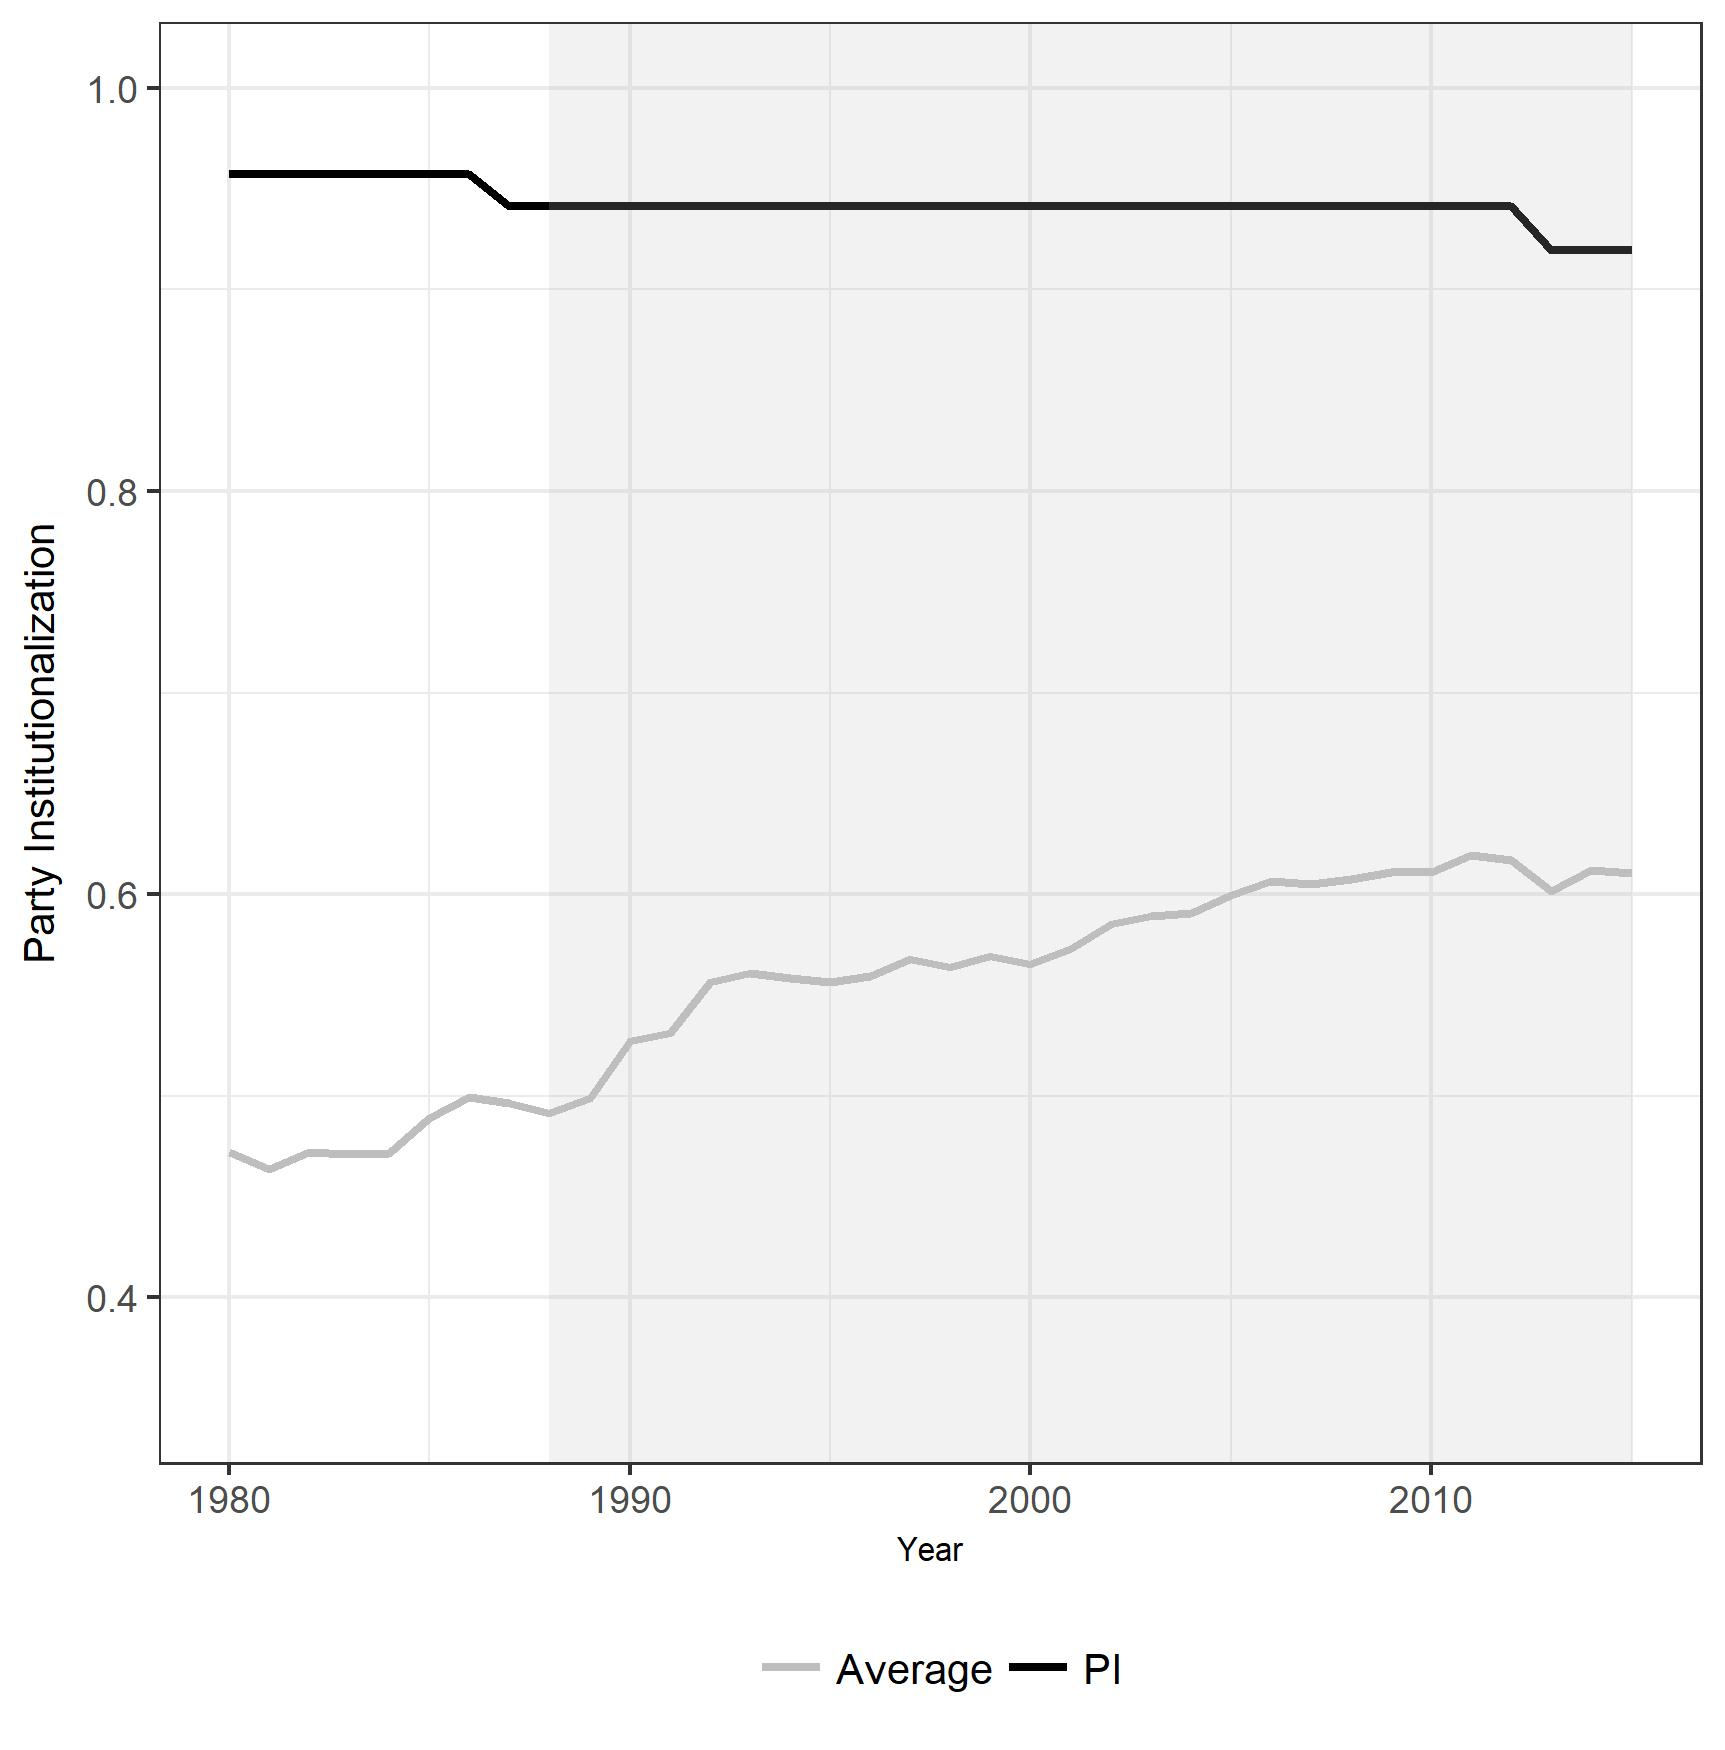
\includegraphics[width=65mm, height=65mm]{france1.jpg}}%
\qquad
\begin{minipage}{2in}%
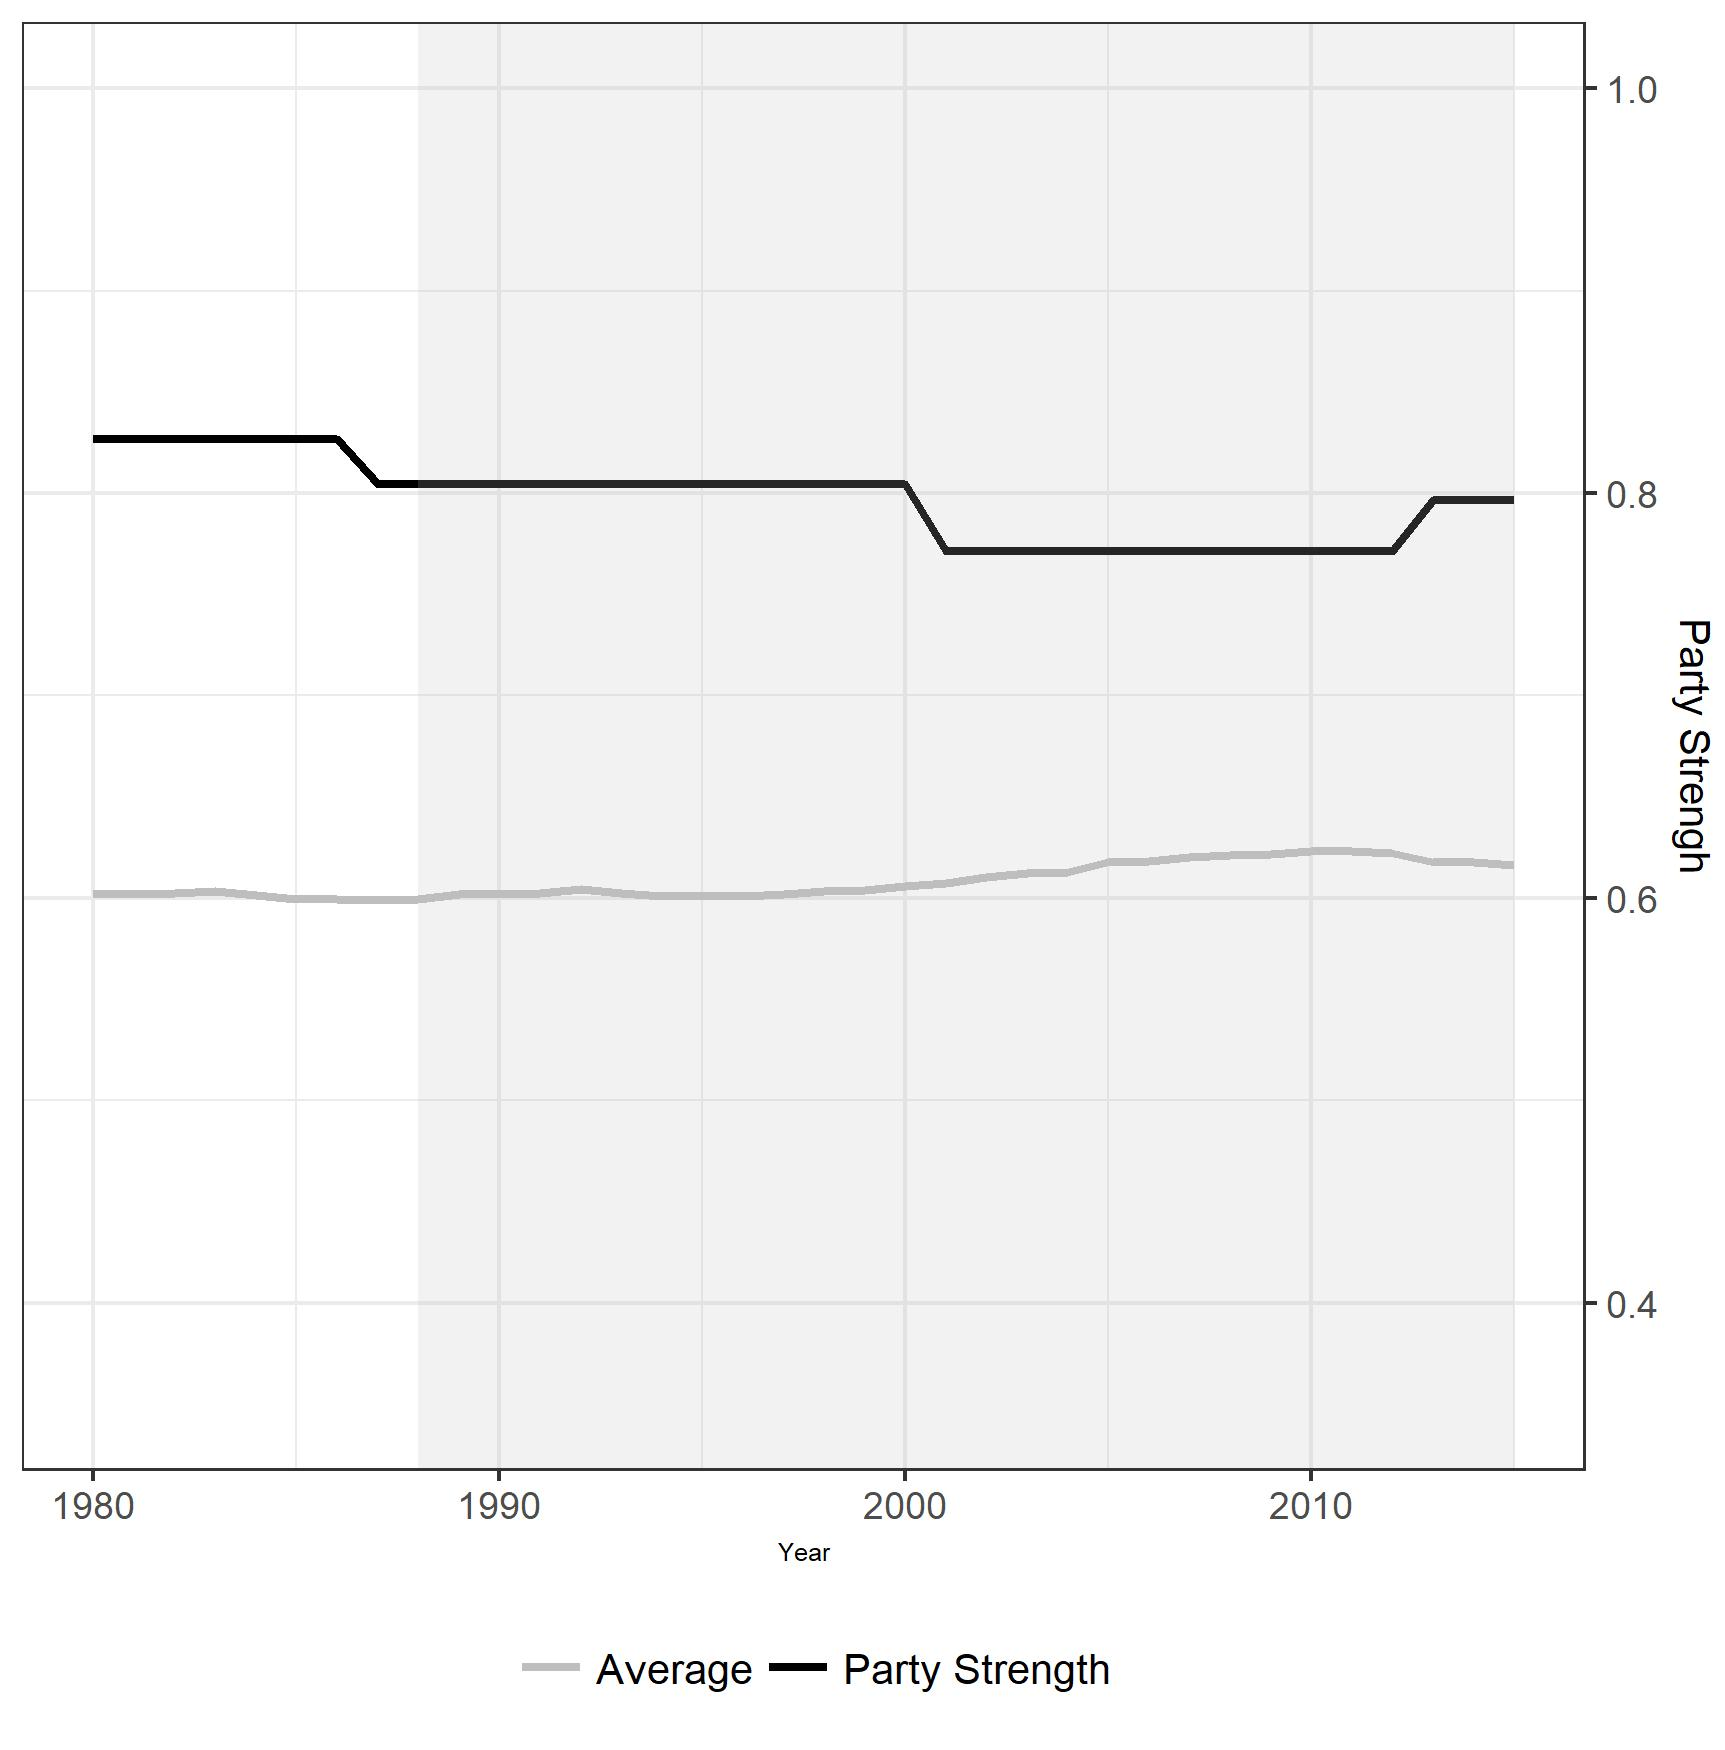
\includegraphics[width=65mm, height=65mm]{france2.jpg}
\end{minipage}%
\caption{French Party Institutionalization and Party Strength}%
\label{francepsi}%
\end{figure}
\par
Although the FN was founded by Jean-Marie Le Pen in 1972, the FN first found limited electoral success in 1986 and 1988. During the 1990s, the FN became more ethno-centric in order to expand its base while at the same time building links to labor unions and making use of state networks \citep{schain1999national}. The party's fortunes declined during the mid-2000s as Nicolas Sarkozy's UMP moved to the right to co-opt some of FN's positions. Further problems  arose for the FN as mainstream parties began actively coordinating against the FN. This resulted in the FN's poorest electoral performance in 2007 with the party only garnering 4.3\% of the vote in the National Assembly and 10.4\% in the presidential election. 
\par
Following the late 2000s decline, Jean-Marie retired and his daughter, Marine, became president of the party. Marine's professional image differs from father's and she has pursued a different electoral strategy. She immediately moved to adapt and re-calibrate the FN to better compete in the party system. This included removing extremely xenophobic content from the party platform and moving the party away from the radical right \citep{shields2013marine} in a move to "de-demonize" the party \citep{mayer2013jean}.\footnote{ Although the FN is commonly referred to as a populist party, the party's manifesto and speeches by Marine Le Pen are not heavily populist. \citet{hawkins2015mapping} score (using 2012 speeches and manifestos) the FN much lower on their scale of populism than many parties commonly thought of as populist.} After Marine's reforms, the FN reclaimed much of its lost support in the 2012 election. Like the case in Austria, the FN had to adapt to become more inclusive and less populist in the face of \textit{institutional hostility}
\par
\subsection*{Populist Capture}
\noindent
\textit{United States}\\
Populist capture is more rare than populist entry or targeting/adaptation and occurs where there is a restrictive electoral system. In restrictive electoral environments, absent system-wide de-institutionalization, the path for populist entrepreneurs is an internal one--i.e. the capture of an existing party. For this to occur at least one party has to be relatively weaker. The most recent example of this phenomenon is the populist capture a political party in the United States by a political outsider -- Donald Trump. The rise of Donald Trump did not happen overnight and the dynamics that lead to his capture of the Republican Party were in motion well before he entered the political scene. 
\par
As can be seen in Figure \ref{usapsi} the level of institutionalization varied greatly across our two measures. Using \textit{PI} the U.S. parties appear highly institutionalized. By contrast, when measured with our party strength index, the parties appears relatively weak. This difference is driven entirely by an indicator measuring centralized control of candidate selection in the \textit{PS} index and its absence in \textit{PI}. Open primaries in the U.S. increase intra-party divisions and provided a opportunity for populists to seize control. 
\begin{figure}[H]%
\centering
\parbox{2.5in}{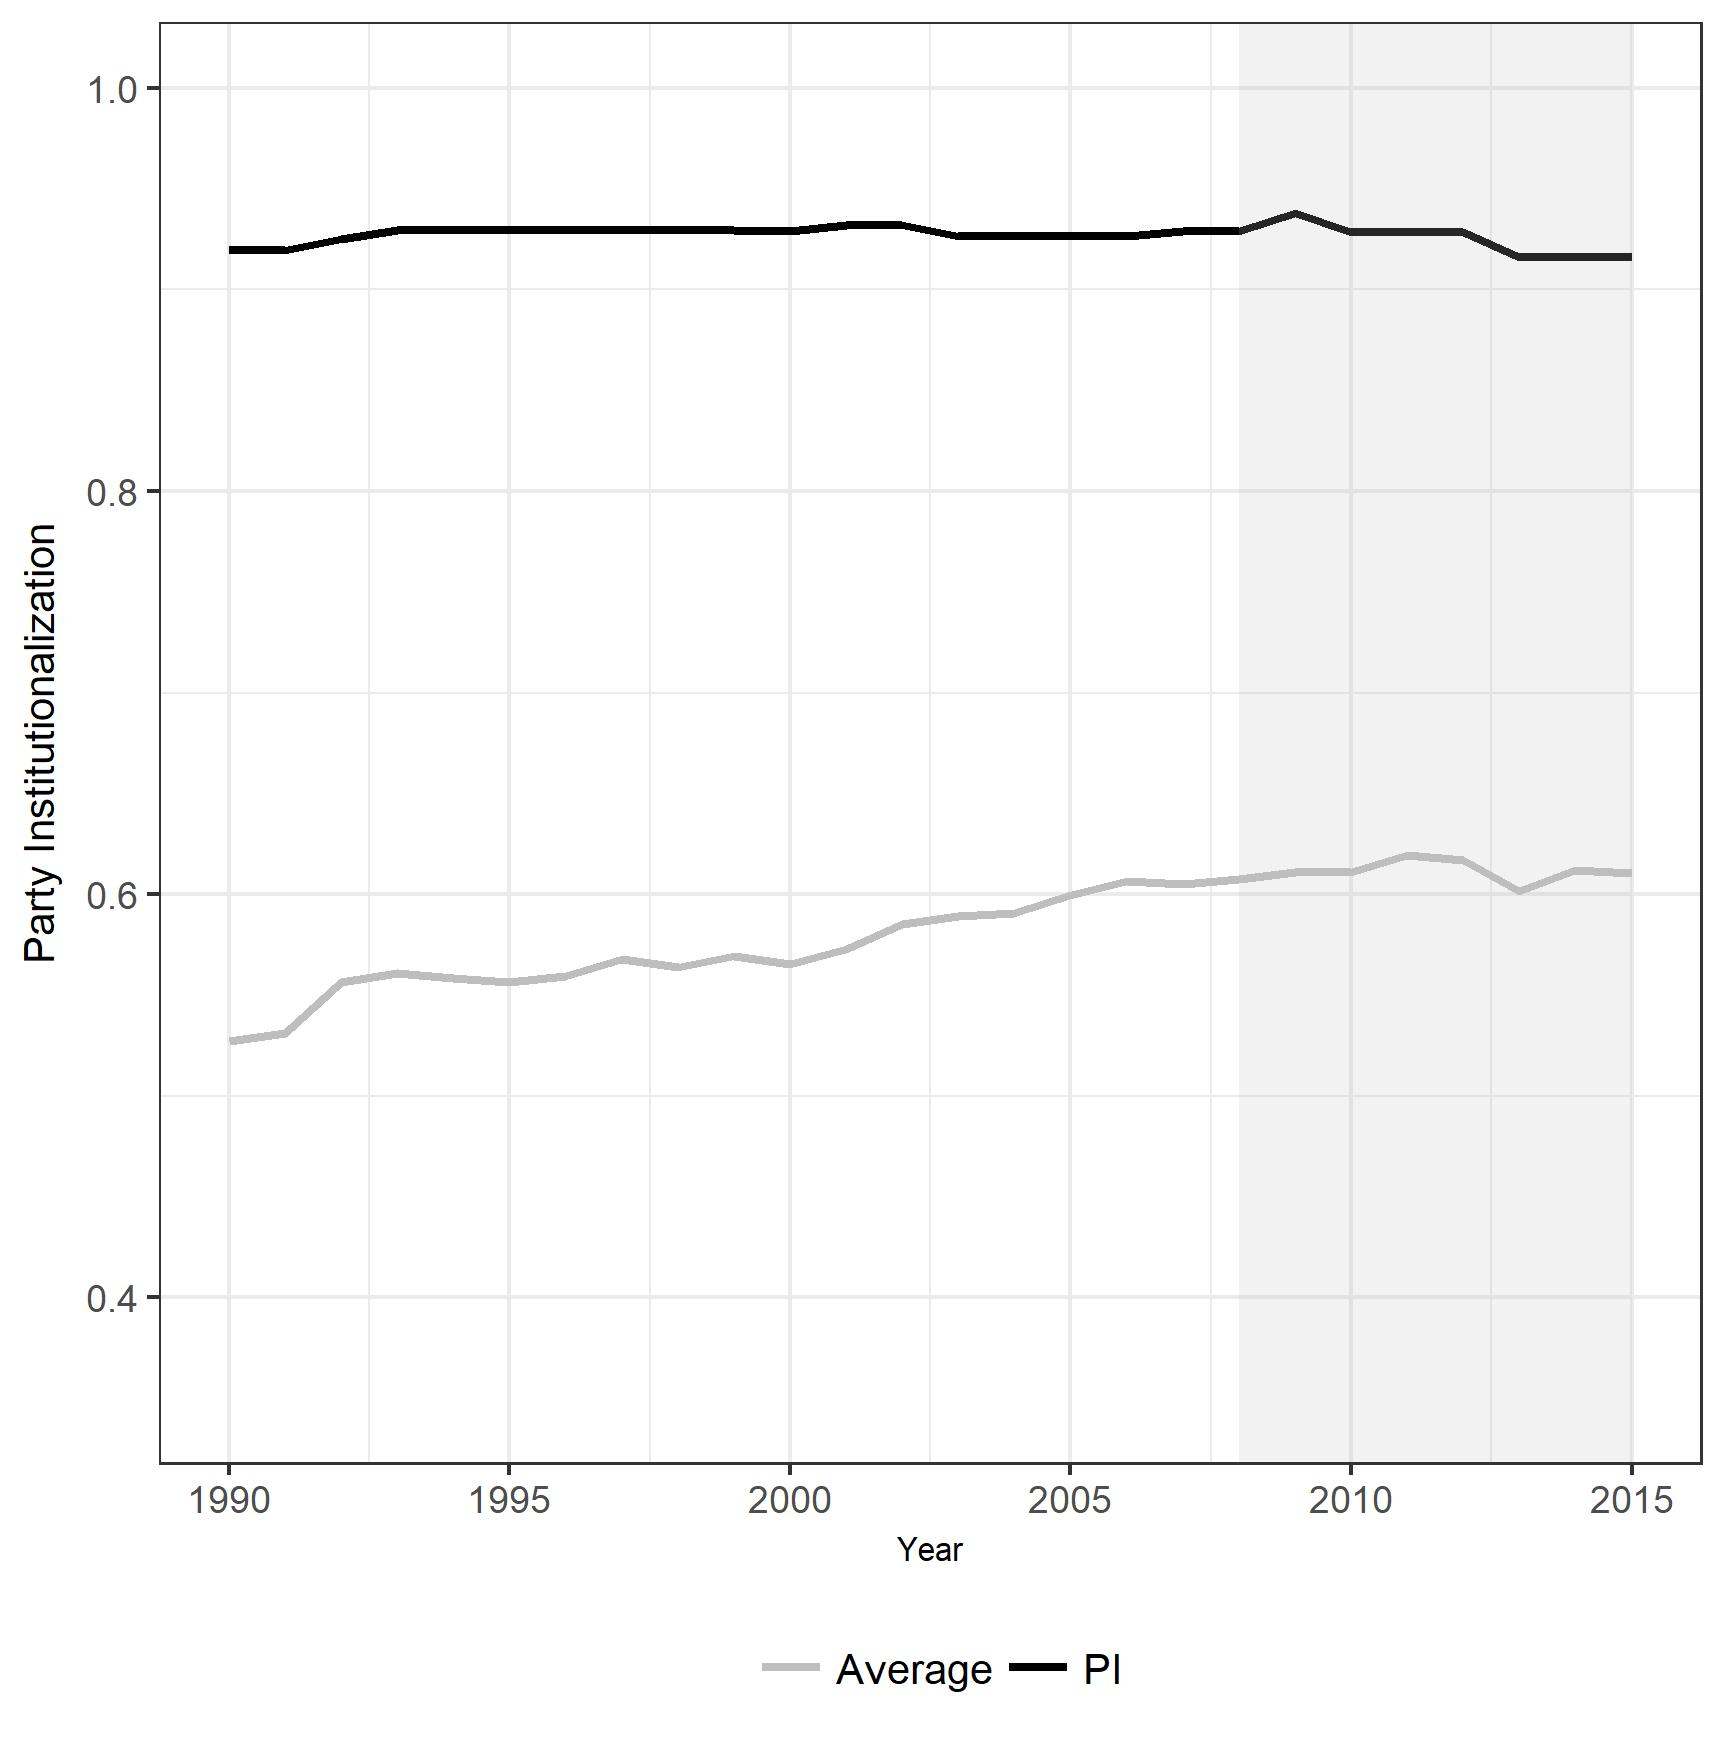
\includegraphics[width=65mm, height=65mm]{usa1.jpg}}%
\qquad
\begin{minipage}{2in}%
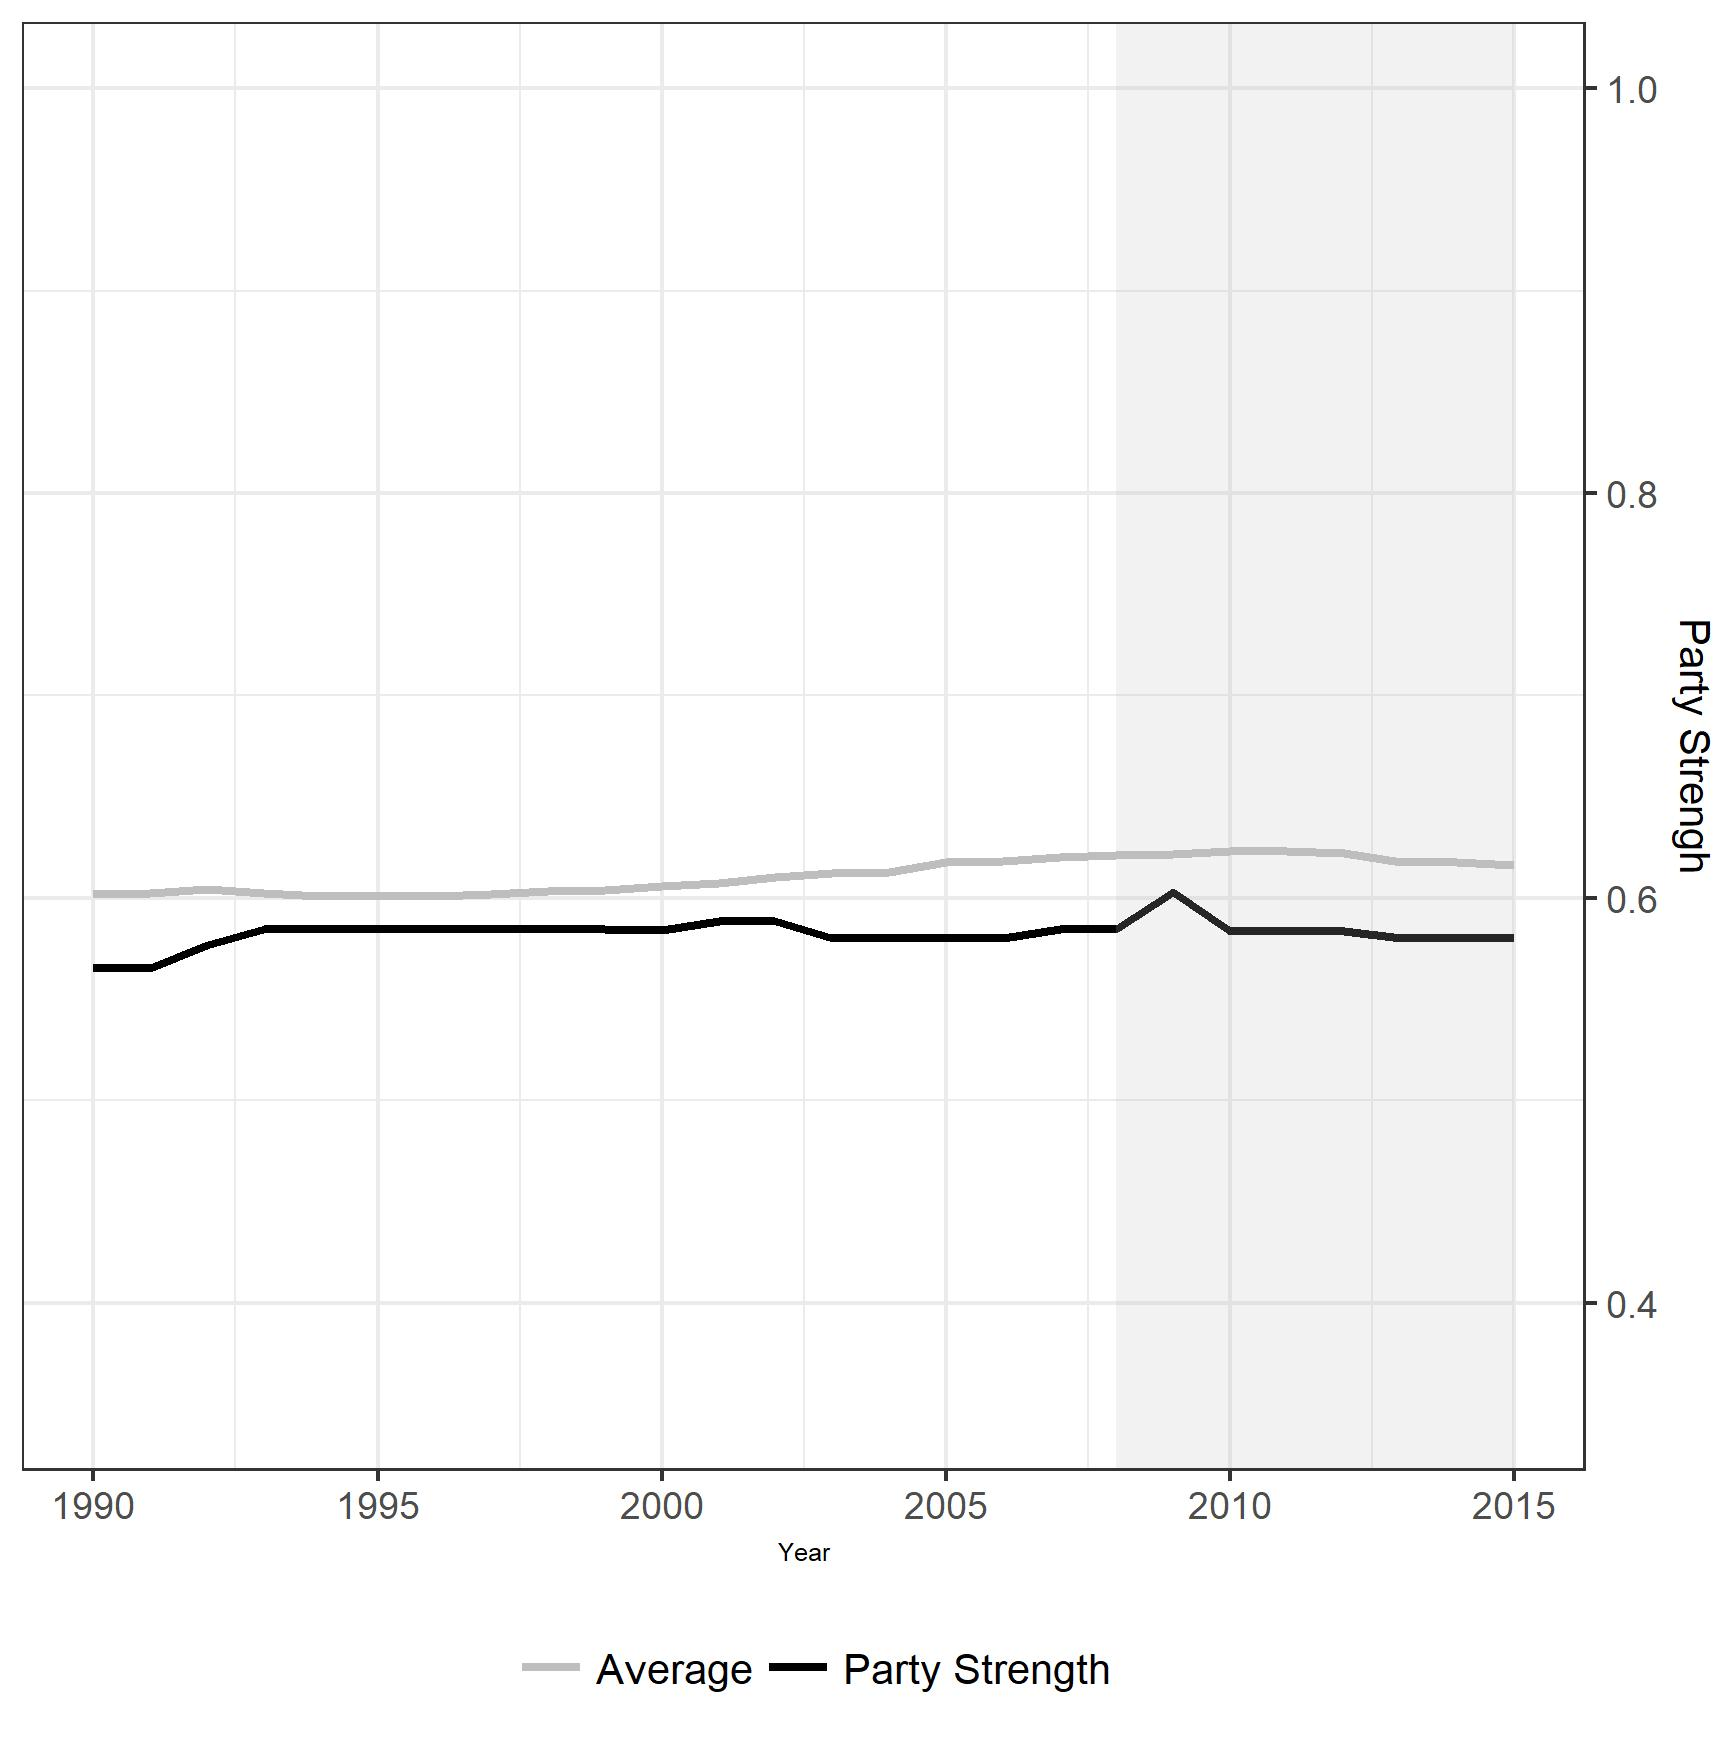
\includegraphics[width=65mm, height=65mm]{usa2.jpg}
\end{minipage}%
\caption{U.S. Party Institutionalization and Party Strength}%
\label{usapsi}%
\end{figure}
\par
The growth of the Tea Party faction within the Republican Party marks the beginning of the populist capture of the party. The presence of the Tea Party created significant problems of collective action at the elite level which would eventually prevent the party from coordinating against Donald Trump. The Tea Party wave of 2010 brought a new set of elites into the Republican Party who held candidate, policy, and legislative preferences that were relatively distant from mainstream party elites. Given the differences in preferences among party elite, intra-party coordination became more difficult. Witness the lack of coherent policy responses by the Republican party vis-\'{a}-vis the Democratic President. Instead of coherent policy responses, Republicans opted for "obstructionism". While many may view this as a selected strategy on the part of the Republicans, we view this as a result of a party paralyzed by the inability to coordinate elite preferences on policy. 
\par
The presence of the Tea Party faction in the Republican Party set the stage for an bitter contest for their party's nomination for the U.S. presidency. The presence of 17 declared candidates for the Republican nomination signals a complete lack of coordination on the part of party elites to select a small set of candidates. This created an opening for a populist to take advantage of the party's decentralized candidate selection model and capture the Republican Party. 
\par
Donald Trump effectively employed populist rhetoric by flaunting the low; frequently using non-elite style of behavior and rhetoric to stand apart from the career politicians. Given the factionalized nature of the party, Republican elites were unable to coordinate response to Trump's populist strategy. After winning the Republican nomination, Trump built on his flaunting of the low rhetoric and introduced elements of Manichean populism--frequently referring to the Democratic Party, Hillary Clinton, and any non-supportive Republican as corrupt or morally suspect. 
\par
After winning the nomination, Donald Trump inherited a party brand and organization, which he was able to use to mobilize voters. Mr. Trump's share of the popular vote is very similar to the same share previous Republican candidates have received in recent history. Polls of voters demonstrate that, as in other elections, voters voted according to their party identification, suggesting that it is unlikely that Trump's populism was key to his Electoral College victory. 
\par
To demonstrate that party capture was key, consider the counterfactual in which Donald Trump tries to enter the electoral arena and challenge both parties as an independent. Mr. Trump would have had no established brand with voters nor any organization to encourage potential supporters to vote. There is very little reason to believe that Donald Trump could have captured the presidency as a true outsider. This suggests that it was Donald Trump the Republican, not Donald Trump the outsider populist, that garnered sufficient electoral support to win a majority of electoral college votes and the Presidency. 


\section*{Discussion and Conclusion}
The purpose of this paper is to establish the plausibility of our theory which posits that institutional hostility is central to understanding the electoral success of populism. We do not argue that institutional hostility is the sole explanation of the success of populism in elections, but we do argue that institutional hostility shapes the degree and pattern of populist competition within a polity. We argue, further, that the rise of populist parties take place via three paths, \textit{ceteris paribus}: \textit{populist entry}, \textit{populist targeting and adaptation}, and \textit{populist capture}. Using cross-national quantitative data as well as exploratory case studies, we come to a number of conclusions. First, as hypothesized the presence of populism is correlated with institutional hostility - as measured by the interaction between the average level of party institutionalization within a party system and the nature of the electoral system. Where the level of institutional hostility is higher we observe lower levels of populism within party systems. Second, populist parties tend to enter or improve their electoral success \textit{after} average strength of existing parties decreases.
\par
This finding is critical to addressing the issue of timing in the causal story of the rise of populist parties. Instead of populism being responsible for the weakening or de-institutionalization of parties, our evidence suggests that party weakening precedes the rise of populism. Lastly, we find institutional hostility shapes the strategies of populist entrepreneurs. In cases where electoral institutions are restrictive, populist parties must either dilute their populism brand to increase their electoral appeal or capitalize on party weaknesses to capture an existing party. When electoral institutions are more permissive, however, populist parties can win power and influence and do not necessarily need to dilute their brand of populism to appeal to more voters.

\par
The evidence provided in this paper provides support for our assertion that the presence of populism within party systems is tied to the level of institutionalization of other political parties in the system. Where parties within a party system are highly institutionalization (on average) populism as a mobilizing strategy appears to be less viable. The implication of these findings points to the necessity of incorporating the party system into theories seeking to explain electoral fortunes of populist parties. Simply stated, theories explaining the variation in the electoral fortunes of populist parties should not separate populism from the party.  
\par
We also emphasize that populism is not a binary concept. While a wide variety of parties or leaders can be referred to as "populist", the extent to which they rely on populist organization or rhetoric varies. The key finding, however, is that higher levels of institutional hostility decreases the payoffs of populism. In essence, political entrepreneurs face a number of potential trade-offs when considering a populist approach to electoral competition. Parties matter -- but when parties are weak, political entrepreneurs can make use of populist rhetoric or organization to compete within the electoral arena. While some populist movements are dominated by exceptional individuals (e.g. Hugo Ch\'{a}vez), populist parties are still parties and function within a system where they must compete against other parties. 
\par
We argue that party institutionalization is key to understanding the electoral success and behavior of populist parties. By studying populism through the lens of political parties we hope to answer four related questions. First, why is populism much more pervasive in party systems outside of Western Europe? One key feature that distinguishes Western European party systems from their counterparts in other regions is the degree of party institutionalization. We argue that systems with more institutionalized parties provide comparatively less fertile soil for the seeds of populism. Second, what explains why economic shocks give rise to populism in some contexts but not others? We also argue that an implication of our theory is that party institutionalization may be an important intervening variable between shocks and populist support. Third, what explains why anti-elite distrust of institutions is represented by populism in many, but not all cases where this sentiment is present? We argue that the explanation lies in political parties — where parties are institutionalized there is less space for proto-populists to take advantage of popular disillusionment. Thus, while the disillusionment exists, high levels of institutional hostility prevents new parties from entering and capitalizing upon the distrust of institutions.
\par
Lastly, why do some populist parties adopt inclusive strategies while others pursue exclusive strategies? We contend that where party institutionalization is high, populists are forced to appeal to limited segments of the population because many voters are already firmly tied to a party -- leading them to develop more narrow targeting strategies which result in more exclusive appeals. 

%%%%%%%%%%%%%%%%%%%%%%%%%%%%%%%%%%%%%%%%%%%%%%%%%%%%%%%%%%%%%
\clearpage
%%%%%%%%%%%%%%%%%%%%%%%%%%%%%%%%%%%%%%%%%%%%%%%%%%%%%%%%%%%%%
\bibliographystyle{apsr}
\bibliography{bib}

\end{document}
